%
% $RCSfile$
%
% Copyright (c) 2005-2006. Christian Heller. All rights reserved.
%
% Permission is granted to copy, distribute and/or modify this document
% under the terms of the GNU Free Documentation License, Version 1.1 or
% any later version published by the Free Software Foundation; with no
% Invariant Sections, with no Front-Cover Texts and with no Back-Cover
% Texts. A copy of the license is included in the section entitled
% "GNU Free Documentation License".
%
% http://www.cybop.net
% - Cybernetics Oriented Programming -
%
% http://www.resmedicinae.org
% - Information in Medicine -
%
% Version: $Revision$ $Date$ $Author$
% Authors: Christian Heller <christian.heller@tuxtax.de>
%

\section{Practical Proof}
\label{practical_proof_heading}

The proof of operatability for the new concepts is given by the
\emph{Cybernetics Oriented Language} (CYBOL), defined according to the
principles of abstraction worked out before, and by the
\emph{Cybernetics Oriented Interpreter} (CYBOI), a knowledge processing system.
In addition, a prototype application called \emph{Res Medicinae}
\cite{resmedicinae} was implemented in CYBOL.

%
% $RCSfile: cybol.tex,v $
%
% Copyright (c) 2002-2007. Christian Heller. All rights reserved.
%
% Permission is granted to copy, distribute and/or modify this document
% under the terms of the GNU Free Documentation License, Version 1.1 or
% any later version published by the Free Software Foundation; with no
% Invariant Sections, with no Front-Cover Texts and with no Back-Cover
% Texts. A copy of the license is included in the section entitled
% "GNU Free Documentation License".
%
% http://www.cybop.net
% - Cybernetics Oriented Programming -
%
% Version: $Revision: 1.2 $ $Date: 2007-08-01 13:59:00 $ $Author: christian $
% Authors: Christian Heller <christian.heller@tuxtax.de>
%

%
% Determine document class specifying the type of document.
%
% Hand over font size and side format.
%
\documentclass[9pt,twoside]{tuxtax}

%
% Input hyphenation list.
%
%%
% $RCSfile: hyphenation.tex,v $
%
% Copyright (c) 2002-2007. Christian Heller. All rights reserved.
%
% Permission is granted to copy, distribute and/or modify this document
% under the terms of the GNU Free Documentation License, Version 1.1 or
% any later version published by the Free Software Foundation; with no
% Invariant Sections, with no Front-Cover Texts and with no Back-Cover
% Texts. A copy of the license is included in the section entitled
% "GNU Free Documentation License".
%
% http://www.cybop.net
% - Cybernetics Oriented Programming -
%
% Version: $Revision: 1.2 $ $Date: 2007-08-01 13:59:00 $ $Author: christian $
% Authors: Christian Heller <christian.heller@tuxtax.de>
%

\hyphenation{abs-trac-tion}
\hyphenation{ac-tu-ally}
\hyphenation{ana-lyst}
\hyphenation{ana-ly-sis}
\hyphenation{an-cient}
\hyphenation{ap-pli-ca-tion}
\hyphenation{aris-to-tle}
\hyphenation{at-tri-bute}
\hyphenation{be-ing}
\hyphenation{ca-te-go-ri-za-tion}
\hyphenation{client}
\hyphenation{com-po-nen-ti-za-tion}
\hyphenation{com-pu-ter}
\hyphenation{con-fi-gure}
\hyphenation{con-nec-ted}
\hyphenation{cy-ber-ne-tics}
\hyphenation{cyboi}
\hyphenation{cybol}
\hyphenation{cybop}
\hyphenation{des-cribed}
\hyphenation{de-sign}
\hyphenation{de-ve-lop-ment}
\hyphenation{dis-crete}
\hyphenation{di-vide}
\hyphenation{do-main}
\hyphenation{dy-na-mic}
\hyphenation{eli-mi-nate}
\hyphenation{eli-mi-nates}
\hyphenation{eli-mi-na-tion}
\hyphenation{en-gi-nee-ring}
\hyphenation{en-vi-ron-ment}
\hyphenation{ex-pert}
\hyphenation{fi-gure}
\hyphenation{fle-xi-bi-li-sie-rung}
\hyphenation{fun-da-men-tal}
\hyphenation{hard-ware}
\hyphenation{hu-man}
\hyphenation{im-ple-men-ta-tion}
\hyphenation{in-he-rit}
\hyphenation{in-he-ri-tance}
\hyphenation{in-ter-pre-ter}
\hyphenation{java}
\hyphenation{know-ledge}
\hyphenation{lan-guage}
\hyphenation{li-ving}
\hyphenation{lo-gi-cal}
\hyphenation{ma-na-ge-ment}
\hyphenation{mea-ning-ful}
\hyphenation{me-cha-nism}
\hyphenation{me-mo-ry}
\hyphenation{me-thod}
\hyphenation{me-thods}
\hyphenation{mo-del-ling}
\hyphenation{na-ture}
\hyphenation{net-work}
\hyphenation{neu-ral}
\hyphenation{neu-ron}
\hyphenation{ne-ver-en-ding-ly}
\hyphenation{open}
\hyphenation{operating}
\hyphenation{ori-en-ted}
\hyphenation{over-come}
\hyphenation{par-ti-cu-lar}
\hyphenation{prin-ci-ple}
\hyphenation{pro-ba-bi-lis-tic}
\hyphenation{pro-ble-ma-tic}
\hyphenation{pro-gram-ming}
\hyphenation{res-pon-sible}
\hyphenation{re-u-sa-bi-li-ty}
\hyphenation{sci-ence}
\hyphenation{server}
\hyphenation{si-mi-lar}
\hyphenation{soft-ware}
\hyphenation{source}
\hyphenation{spe-cia-li-za-tion}
\hyphenation{spe-ci-fied}
\hyphenation{sta-tic}
\hyphenation{sta-ti-cally}
\hyphenation{sto-chas-tic}
\hyphenation{stone-on-stone}
\hyphenation{struc-ture}
\hyphenation{strug-gling}
\hyphenation{subs-ti-tu-ting}
\hyphenation{su-per-flu-ous}
\hyphenation{sup-ply-ing}
\hyphenation{sys-tem}
\hyphenation{taeu-schungs-ver-such}
\hyphenation{temp-lates}
\hyphenation{tes-ting}
\hyphenation{thin-king}
\hyphenation{un-en-li-vened}
\hyphenation{un-sa-tis-fy-ing}
\hyphenation{va-ry-ing}
\hyphenation{weigh-ted}
\hyphenation{zu-kunfts-si-che-re}


%
% Define text macros.
%
\def\placemacro{Ilmenau}
\def\datemacro{2007-07-31}
\def\authormacro{Christian Heller}
\def\titlemacro{Cybernetics Oriented Language (CYBOL)}
\def\subtitlemacro{An interpretable Knowledge Modelling- and Programming Language}
\def\versionmacro{Version 2.0, Draft \datemacro}

%
% Enable special indexing commands.
% Generate contents, glossary and memo entries.
%
% Required package: makeidx
%
\makeindex

%
% This document describes the Cybernetics Oriented Language (CYBOL).
%
% Author: Christian Heller <christian.heller@tuxtax.de>
%
\begin{document}
    % Set sans serif font.
    \sffamily
    % Set page numbering to roman numbers.
    \pagenumbering{roman}
    %
% $RCSfile: cover.tex,v $
%
% Copyright (c) 2002-2007. Christian Heller. All rights reserved.
%
% Permission is granted to copy, distribute and/or modify this document
% under the terms of the GNU Free Documentation License, Version 1.1 or
% any later version published by the Free Software Foundation; with no
% Invariant Sections, with no Front-Cover Texts and with no Back-Cover
% Texts. A copy of the license is included in the section entitled
% "GNU Free Documentation License".
%
% http://www.cybop.net
% - Cybernetics Oriented Programming -
%
% Version: $Revision: 1.1 $ $Date: 2007-07-17 20:02:36 $ $Author: christian $
% Authors: Christian Heller <christian.heller@tuxtax.de>
%

%
% Defines the title page.
%
% \title and \author (and optionally \date) must be specified!
%
% Sets the page style of the first page to empty
% that is no header or footer will be shown.
%
\begin{titlepage}
    \title{
        Cybernetics Oriented Language 1.0\\
        (CYBOL)\\
        \vspace{1cm}
        % \textmd sets medium weight (default), which is the opposite of boldface.
        \normalsize{\textmd{An interpretable Knowledge Modelling- and Programming Language\\}}
    }
    \author{
        \date{
        }
    }
\end{titlepage}

    \maketitle
    % Avoid header, footer and page number.
    \thispagestyle{empty}
    \title{Flexible Software Architectures for Presentation Layers demonstrated on Medical Documentation with Episodes and Inclusion of Topological Report}
\author{Jens Bohl \(<\)info@jens-bohl.de\(>\)\\
Torsten Kunze \(<\)zone3@gmx.de\(>\)\\
Christian Heller \(<\)christian.heller@tu-ilmenau.de\(>\)\\
Ilka Philippow \(<\)ilka.philippow@tu-ilmenau.de\(>\)}
\institute{
Technical University of Ilmenau\\
Faculty for Computer Science and Automation\\
Institute for Theoretical and Technical Informatics\\
PF 100565, Max-Planck-Ring 14, 98693 Ilmenau, Germany\\
http://www.tu-ilmenau.de, fon: +49-(0)3677-69-1230, fax: +49-(0)3677-69-1220}
\maketitle

    \newpage{\pagestyle{empty}\clearpage}
    \thispagestyle{empty}
    %
% $RCSfile: copyright.tex,v $
%
% Copyright (C) 2002-2008. Christian Heller.
%
% Permission is granted to copy, distribute and/or modify this document
% under the terms of the GNU Free Documentation License, Version 1.1 or
% any later version published by the Free Software Foundation; with no
% Invariant Sections, with no Front-Cover Texts and with no Back-Cover
% Texts. A copy of the license is included in the section entitled
% "GNU Free Documentation License".
%
% http://www.cybop.net
% - Cybernetics Oriented Programming -
%
% http://www.resmedicinae.org
% - Information in Medicine -
%
% Version: $Revision: 1.1 $ $Date: 2008-08-19 20:41:06 $ $Author: christian $
% Authors: Christian Heller <christian.heller@tuxtax.de>
%

\small{Cataloging-in-Publication Data\\
    Christian Heller.\\
    Cybernetics Oriented Programming (CYBOP):\\
    An Investigation on the Applicability of Inter-Disciplinary Concepts\\
    to Software System Development\\
    Ilmenau: Tux Tax, 2006\\
    ISBN-10: 3-9810898-0-4\\
    ISBN-13: 978-3-9810898-0-6}\\

\small{Information on Ordering this book\\
    http://www.tuxtax.de, http://www.cybop.net}

\small{Written as Dissertation\\
    Supervisor 1: Prof. Dr.-Ing. habil. Ilka Philippow (Chair), Technical University of Ilmenau\\
    Supervisor 2: Prof. Dr.-Ing. habil. Dietrich Reschke, Technical University of Ilmenau, Germany\\
    Supervisor 3: Mark Lycett (PhD), Brunel University, Great Britain\\
    Submission: 2005-12-12; Presentation: 2006-10-04}

\small{Copyright \textcopyright\ 2002-2006. \authormacro. All rights reserved.}

%> \small{Translation: Christian Heller}\\ %\"Ubersetzung:
%\small{Sponsoring Editor: ??}\\ %Lektorat:
%\small{Acquisitions Editor: ??}\\
%\small{Marketing Manager: ??}\\
%\small{Marketing Assistant: ??}\\
%\small{Editorial Assistant: ??}\\
%\small{Editorial/ Production Supervision: ??}\\
%\small{Production Editor: Christian Heller}\\ %Produktion:
%\small{Production Service: ??}\\ %Produktion:
%\small{Manuscript Editor: ??}\\
%\small{Interior Illustration: ??}\\
%\small{Interior Design: ??}\\
\small{Cover Illustration: TSAMEDIEN, D\"usseldorf}\\ %Umschlaggrafik:
%\small{Cover Design: Christian Heller}\\ %Umschlaggestaltung:
%\small{Print Buyer: ??}\\
%\small{Project Coordinator: ??}\\
%> \small{Typesetting: Christian Heller, set in Times 9.5 pt font with \LaTeX\ using Kile under Linux}\\ %Satz:
%\small{Cover Printing: ??}\\
\small{Printing and Binding: Offizin Andersen Nex\"o, Leipzig/ Zwenkau} %Belichtung, Druck und Bindung:

\small{Permission is granted to copy, distribute and/or modify this document
    under the terms of the GNU Free Documentation License, Version 1.2
    or any later version published by the Free Software Foundation;
    with no Invariant Sections, with no Front-Cover Texts and with no
    Back-Cover Texts. A copy of the license is included in the section
    entitled "GNU Free Documentation License".}

\small{Trademark Credits\\
    Most of the software-, hardware- and product names used in this document
    are also trademarks or registered trademarks of their respective owners.
%    Adobe is a trademark of Adobe Systems, Incorporated.\\
%    AIX is a trademark of International Business Machines Corporation.\\
%    Arial\textregistered\ is a registered trademark of the Monotype Corporation in the United States and other countries.\\
%>    CICS is a trademark of International Business Machines Corporation.\\
%    CICS/ESA is a trademark of International Business Machines Corporation.\\
%    CorelDRAW\texttrademark\ is a trademark or registered trademark of Corel Corporation or Corel Corporation Limited.\\
%>    DB2 is a trademark of International Business Machines Corporation.\\
%    DFSMS is a trademark of International Business Machines Corporation.\\
%    DFSORT is a trademark of International Business Machines Corporation.\\
%    Energy Star\textregistered\ and the Energy Star logo\textregistered\ are registered marks of the United States Environmental Protection Agency in the United States and other countries. Details on the proper use of the marks are explained in the "Guidelines for Proper use of the Energy Star\textregistered\ Name and International Logo".\\
%>    Ethernet is a registered trademark of Xerox Corporation.\\
%>    IBM\textregistered\ is a registered trademark of International Business Machines Corporation.\\
%    IBM Warp Server\textregistered\ is a registered trademark of International Business Machines Corporation.\\
%    IMS is a trademark of International Business Machines Corporation.\\
%    IMS/ESA is a trademark of International Business Machines Corporation.\\
%>    Intel is a registered trademark of Intel Corporation in the United States and other countries.\\
%>    Java\texttrademark\ and all Java-based trademarks are trademarks of Sun Microsystems, Inc. in the United States and other countries.\\
%    Language Environment is a trademark of International Business Machines Corporation.\\
%>    Microsoft\textregistered\ is a registered trademark of Microsoft Corporation in the United States and other countries.\\
%    MS Windows\textregistered\ is a registered trademark of Microsoft Corporation in the United States and other countries.\\
%    MS-DOS\textregistered\ is a registered trademark of Microsoft Corporation in the United States and other countries.\\
%    MVS is a trademark of International Business Machines Corporation.\\
%    Netscape is a trademark of Netscape Communications Corporation in the United States and other countries.\\
%    Netscape Navigator is a trademark of Netscape Communications Corporation in the United States and other countries.\\
%    Netware\textregistered\ is a registered trademark of Novell Corporation.\\
%    Novell\textregistered\ is a registered trademark of Novell Corporation.\\
%    OpenEdition is a trademark of International Business Machines Corporation.\\
%    Opera\texttrademark\ is a trademark of Opera Software ASA.\\
%    Operating System/2\textregistered\ (OS/2) is a registered trademark of International Business Machines Corporation.\\
%    *Pantone, Inc. is a check-standard trademark for color.\\
%>    Pentium is a registered trademark of Intel Corporation in the United States and other countries.\\
%>    PostScript is a trademark of Adobe Systems, Incorporated.\\
%    RACF is a trademark of International Business Machines Corporation.\\
%    System/390 is a trademark of International Business Machines Corporation.\\
%>    Unicode is a trademark of the Unicode Consortium.\\
%>    UNIX\textregistered\ is a registered trademark of The Open Group in the United States and other countries.\\
%    VisualAge is a trademark of International Business Machines Corporation.\\
%>    Windows\textregistered\ is a registered trademark of Microsoft Corporation in the United States and other countries.\\
%    Windows NT\textregistered\ is a registered trademark of Microsoft Corporation in the United States and other countries.\\
%    z/OS is a trademark of International Business Machines Corporation.\\
%>    Other company-, product- or service names may be the trademarks or service marks of others.\\
}

\small{Donations\\
    Companies planning to publish this work on a grand scale are asked to
    notify the author \(<\)christian.heller@tuxtax.de\(>\) and to consider
    donating some of their sales revenues, which will be used exclusively for
    the CYBOP and Res Medicinae free software projects.}

\small{Text printed on recycled and acid-free paper.}

\small{Printed in Germany}

    \newpage{\pagestyle{empty}\cleardoublepage}
    % Avoid header, footer and page number.
    \thispagestyle{empty}
    %
% $RCSfile: dedication.tex,v $
%
% Copyright (c) 2002-2007. Christian Heller. All rights reserved.
%
% Permission is granted to copy, distribute and/or modify this document
% under the terms of the GNU Free Documentation License, Version 1.1 or
% any later version published by the Free Software Foundation; with no
% Invariant Sections, with no Front-Cover Texts and with no Back-Cover
% Texts. A copy of the license is included in the section entitled
% "GNU Free Documentation License".
%
% http://www.cybop.net
% - Cybernetics Oriented Programming -
%
% Version: $Revision: 1.1 $ $Date: 2007-07-17 20:02:36 $ $Author: christian $
% Authors: Christian Heller <christian.heller@tuxtax.de>
%

\vspace*{3cm}
\begin{center}
    To all Hackers (not Crackers) who stick to the ?? Hackers' Codex\\
    and contribute with great Enthusiasm to the Free Software Code Base\\
    of the Open Source Community
\end{center}

    \newpage{\pagestyle{empty}\cleardoublepage}
    \tableofcontents
    \newpage{\pagestyle{empty}\cleardoublepage}
    % Set roman font.
    \rmfamily
    %
% $RCSfile: preface.tex,v $
%
% Copyright (C) 2002-2008. Christian Heller.
%
% Permission is granted to copy, distribute and/or modify this document
% under the terms of the GNU Free Documentation License, Version 1.1 or
% any later version published by the Free Software Foundation; with no
% Invariant Sections, with no Front-Cover Texts and with no Back-Cover
% Texts. A copy of the license is included in the section entitled
% "GNU Free Documentation License".
%
% http://www.cybop.net
% - Cybernetics Oriented Programming -
%
% http://www.resmedicinae.org
% - Information in Medicine -
%
% Version: $Revision: 1.1 $ $Date: 2008-08-19 20:41:08 $ $Author: christian $
% Authors: Christian Heller <christian.heller@tuxtax.de>
%

\chapter*{Preface\markboth{Preface}{Preface}}
\label{preface_heading}
\addcontentsline{toc}{chapter}{Preface}

\begin{flushright}
    \textsl{
        I slept and dreamt that Life was Joy.\\
        I awoke and saw that Life was Service.\\
        I acted and behold, Service was joy.
    }\\
    \textsc{Rabindranath Tagore}
\end{flushright}

%
% $RCSfile: prologue.tex,v $
%
% Copyright (C) 2002-2008. Christian Heller.
%
% Permission is granted to copy, distribute and/or modify this document
% under the terms of the GNU Free Documentation License, Version 1.1 or
% any later version published by the Free Software Foundation; with no
% Invariant Sections, with no Front-Cover Texts and with no Back-Cover
% Texts. A copy of the license is included in the section entitled
% "GNU Free Documentation License".
%
% http://www.cybop.net
% - Cybernetics Oriented Programming -
%
% http://www.resmedicinae.org
% - Information in Medicine -
%
% Version: $Revision: 1.2 $ $Date: 2008-09-07 15:36:07 $ $Author: christian $
% Authors: Christian Heller <christian.heller@tuxtax.de>
%

\section*{Prologue}
\label{prologue_heading}
%\addcontentsline{toc}{section}{Prologue}

To me, basically, there are two ways to deal with a scientific subject:

\begin{enumerate}
    \item The deepened investigation on a special area aiming to find
        completely new phenomenons
    \item The systematic subsumption of multiple known aspects of one or many
        disciplines aiming to find new cross-correlations and ideas
\end{enumerate}

Both approaches may lead to new theories, methods and concepts. And both may use
laboratory trials to find and prove their theories. This work follows the second
approach. The idea behind is, simply spoken, to steal ideas from nature and
various fields of science, and to apply them to software design.

\emph{Laboratory Trials} are what \emph{Coding} is in informatics -- experiment
and proof of operability, at the same time. Some information scientists have
the opinion that coding weren't \emph{scientific} enough and not necessary to
create new theories or to achieve good results. I doubt this. In my opinion,
there are things that can only be found when actually implementing ideas in a
computer language. And in the end, a theory is worth much more when having been
proven in practice. This document contains proven ideas that were growing in my
mind over the last few years, while dealing with topics such as:

\begin{itemize}
    \item[-] Structured- and Procedural Programming
    \item[-] Object Oriented Programming
    \item[-] Design Patterns and Frameworks
    \item[-] Component Based Design and Agents
    \item[-] Ontology Structured Domain Knowledge
    \item[-] Document- and User Interface Markup
    \item[-] Persistence Mechanisms
    \item[-] System Communication
    \item[-] Operating System Concepts
\end{itemize}

The usage of typical buzzwords could not quite be avoided in this work, yet do
I hope that the ideas and results are nevertheless explained straightforward and
well enough to be really useful to some other developers out there.

This document claims to be an \emph{Academic Paper}. To all practitioners who do
not want to read it for that reason, I would like to point out that each and
every concept in it arose from practice, that is coding. Like most developers,
I started up with only a few lines of code in one Java class, later extended to
more classes, a whole framework and so on. Whenever I stumbled over difficulties,
I thought through and improved my current design by applying patterns recommended
by several software development Gurus. It was only when I realised that even
those concepts were not sufficient, that I made up my own. They are entitled
\emph{Cybernetics Oriented Programming} (CYBOP), because most ideas behind them
stem from nature.

Finally, this document has become my thesis, written to earn a doctorate
(Dr.-Ing./ PhD) in Informatics/ Software Engineering. You may wonder why I
release it under the \emph{Free Documentation License} (FDL). Well, I'm a full
supporter of the idea of \emph{Free Knowledge}, \emph{Free Software}, a
\emph{Society free of Patents} which are only hindering its development. There
are three reasons that have contributed to my decision:

\begin{enumerate}
    \item Hope to get helpful \emph{Feedback} from readers
    \item Trust in the scientific \emph{Fairness} of colleagues, worldwide, to
        properly reference this document even though it is licensed under the FDL
    \item Wish to contribute to the open source movement \emph{now} (and not in
        some years when the document might reach a more stable version), to
        speed up its successful development
\end{enumerate}

This is a growing document undergoing steady development. It is not and doesn't
claim to be free of errors nor to contain the only possible way for application
system development. So, if you find errors of whatever kind or have any helpful
ideas or constructive criticism, then please contribute them to
\(<\)christian.heller@tuxtax.de\(>\) or to the CYBOP developers mailing list
\(<\)cybop-developers@lists.berlios.de\(>\)!

%
% $RCSfile: scientific_progress.tex,v $
%
% Copyright (C) 2002-2008. Christian Heller.
%
% Permission is granted to copy, distribute and/or modify this document
% under the terms of the GNU Free Documentation License, Version 1.1 or
% any later version published by the Free Software Foundation; with no
% Invariant Sections, with no Front-Cover Texts and with no Back-Cover
% Texts. A copy of the license is included in the section entitled
% "GNU Free Documentation License".
%
% http://www.cybop.net
% - Cybernetics Oriented Programming -
%
% http://www.resmedicinae.org
% - Information in Medicine -
%
% Version: $Revision: 1.1 $ $Date: 2008-08-19 20:41:08 $ $Author: christian $
% Authors: Christian Heller <christian.heller@tuxtax.de>
%

\section*{Scientific Progress}
\label{scientific_progress_heading}
%\addcontentsline{toc}{section}{Scientific Progress}

An \emph{Abstraction} allows to capture the real world by representing it in
simplified models. Such models contain only the essential aspects of a special
domain. Any unimportant nuances, in the considered context, are neglected.
Correct abstract models is what makes science easy. Good science \emph{can} be
\emph{easy}. If it is not, then probably either:

\begin{itemize}
    \item[-] there is a \emph{mistake} in the model
    \item[-] it is not fully \emph{understood} by the scientist him/ herself
    \item[-] the explaining person wants to \emph{keep back} knowledge, making
        others look clueless
\end{itemize}

One of the biggest hindrances to scientific progress is too much or false
respect for existing solutions. No theory/ model/ concept is ever finished;
no document/ software/ product is ever fully completed. There is always room
for improvements. In the end, it is all just a person's subjective perception
and an arbitrary, abstract extract of the real world.

It is always worth reviewing and questionning everything in depth, again and
again. Standstill means regress. The best example showing how to work around
these criticisms is the \emph{Free and Open Source Software} (FOSS) movement
where all the time, existing solutions are rewritten, to be improved.

%
% $RCSfile: software_patents.tex,v $
%
% Copyright (C) 2002-2008. Christian Heller.
%
% Permission is granted to copy, distribute and/or modify this document
% under the terms of the GNU Free Documentation License, Version 1.1 or
% any later version published by the Free Software Foundation; with no
% Invariant Sections, with no Front-Cover Texts and with no Back-Cover
% Texts. A copy of the license is included in the section entitled
% "GNU Free Documentation License".
%
% http://www.cybop.net
% - Cybernetics Oriented Programming -
%
% http://www.resmedicinae.org
% - Information in Medicine -
%
% Version: $Revision: 1.1 $ $Date: 2008-08-19 20:41:08 $ $Author: christian $
% Authors: Christian Heller <christian.heller@tuxtax.de>
%

\section*{Software Patents}
\label{software_patents_heading}
%\addcontentsline{toc}{section}{Software Patents}

This work is about software. Software abstracts the real world, its items and
processes, and it can store these information and their relations which make up
actual \emph{Knowledge}. In the modern, so-called \emph{Information Society},
it becomes more and more important to have \emph{free} access to external
knowledge. This is an \emph{essential} human right and will decide about the
future living quality of people.

So much the important it is to \emph{prohibit} the application of patents to
software! They make an exclusive club of large companies own the rights on
banal, ordinary, day-to-day algorithms and methods that many people use. And,
they thereby kill any new ideas and hinder research efforts that depend on
these basic algorithms. If \emph{Software Patents} and patents on
\emph{Computer Implemented Inventions} (CII) got introduced, any free software
developer and especially \emph{Small- and Medium Sized Enterprises} (SME), the
driving force of innovation, could not unfold their full potential anymore,
since much of their time and effort would then have to go into patent inquiries
and costly legal disputes.

Software patents are dangerous for the free development of thoughts! Certain
lobbies exert an increasing influence on politics and push members of
parliaments to agitate and vote in their interest. Since probably every reader
of this document has an interest in informatics, every reader is also affected
by the software patent enforcement. But everybody can do something about it,
not only in Europe! Express your protest and sign the petition at \cite{ffii}!

%
% $RCSfile: free_publishing.tex,v $
%
% Copyright (C) 2002-2008. Christian Heller.
%
% Permission is granted to copy, distribute and/or modify this document
% under the terms of the GNU Free Documentation License, Version 1.1 or
% any later version published by the Free Software Foundation; with no
% Invariant Sections, with no Front-Cover Texts and with no Back-Cover
% Texts. A copy of the license is included in the section entitled
% "GNU Free Documentation License".
%
% http://www.cybop.net
% - Cybernetics Oriented Programming -
%
% http://www.resmedicinae.org
% - Information in Medicine -
%
% Version: $Revision: 1.1 $ $Date: 2008-08-19 20:41:06 $ $Author: christian $
% Authors: Christian Heller <christian.heller@tuxtax.de>
%

\section*{Free Publishing}
\label{free_publishing_heading}
%\addcontentsline{toc}{section}{Free Publishing}

Reputation in the scientific world strongly depends on the number of
publications in scientific journals, conference proceedings, magazines etc., of
which some have greater kudos, some less. A \emph{Philosophiae Doctor} (PhD)
student, for example, is expected to publish in some of the \emph{acknowledged}
journals, in order to be conferred a doctorate. The grant of project fundings
by local-, national- or \emph{European Union} (EU) governements and sponsorship
of a professor's department at university depend on it as well. Some unfair
practices and shortcomings of the current system of publication shall therefore
be mentioned here. There are at least four disadvantages of publishing in
scientific journals. An author:

\begin{itemize}
    \item is almost always forced to assign his copyright to the publisher;
    \item has very little chance of publishing completely new ideas, since
        evaluators (which are to guarantee a certain \emph{scientific level})
        sieve those which seem too crazy or are unknown to them and do not
        match state-of-the-art science, so that really new ideas can hardly
        become popular in this way;
    \item has to wait many months before being informed about article
        acceptance, sometimes further months to presentation at a conference
        and yet more months until a journal/ proceedings are finally available
        -- which, besides the unfine delay, is enough time for an evaluator to
        adapt the best ideas and publish them in a modified form before;
    \item and everyone else have to pay money for receiving journals (even for
        the one containing the author's own work), or become a member of
        certain scientific societies for some discount -- which means that the
        work is not freely accessible.
\end{itemize}

Further, there is something often labelled \emph{Citation Mafia}. Whether an
article gets published in a journal or not depends on it being accepted by a
number of reviewers (normally three). In order to avoid personal battles, the
article author never gets to know the evaluators' names or proficiency and has
to blindly rely on the \emph{good taste} of a conference's program committee.
However, evaluators, although tied to ethical standards, often seem to have
their list of \emph{friends} or seem to just prefer authors who have already
published elsewhere, leading to circles of scientists citing each other, quite
independent from the quality of their papers. Logically, also here, there are a
number of disadvantages:

\begin{itemize}
    \item Young scientists have a hard life and need a long time for getting
        their articles accepted, independent from how innovative they are.
    \item Mafioso scientists often warm up old stories or deliver well-formulated,
        but rubbish articles not earning the predicate \emph{scientific}.
\end{itemize}

Don't ask for proof -- I don't have it. But almost everybody in the scientific
business knows about these issues. Unfortunately, only few people \cite{jobb}
talk about- or try to change them. Obviously, many scientists prefer to either
play the same old game or are scared of personal disadvantages. However, it
feels like increasingly more researchers, in particular the new generation,
become aware that these drawbacks hinder scientific progress and new solutions
need to be found. Well, there is free online journals such as the
\emph{Journal of Free and Open Source Medical Computing} (JOSMC) \cite{josmc}
or the \emph{BioMed Central} (BMC) \cite{bmc} publisher, where research
articles are: \textit{free to access immediately, peer reviewed,
citation-tracked \ldots}

Although this document cannot deliver solutions to the above-mentioned
problems, it mentioned those to inform the reader and spur further discussion.
Supportive actions in this process would be that:

\begin{itemize}
    \item scientists acknowledge no-cost entry open source conferences like
        LinuxTag \& Co. \cite{linuxtag} as alternatives to traditional ones
    \item professors more readily accept citations of free knowledge sources
        such as Wikipedia \cite{wikipedia} in scientific works of their students
    \item students and scientists publish their works (code and documentation)
        under open source licenses
\end{itemize}

%
% $RCSfile: new_science.tex,v $
%
% Copyright (C) 2002-2008. Christian Heller.
%
% Permission is granted to copy, distribute and/or modify this document
% under the terms of the GNU Free Documentation License, Version 1.1 or
% any later version published by the Free Software Foundation; with no
% Invariant Sections, with no Front-Cover Texts and with no Back-Cover
% Texts. A copy of the license is included in the section entitled
% "GNU Free Documentation License".
%
% http://www.cybop.net
% - Cybernetics Oriented Programming -
%
% http://www.resmedicinae.org
% - Information in Medicine -
%
% Version: $Revision: 1.1 $ $Date: 2008-08-19 20:41:07 $ $Author: christian $
% Authors: Christian Heller <christian.heller@tuxtax.de>
%

\section*{New Science}
\label{new_science_heading}
%\addcontentsline{toc}{section}{New Science}

It was end of October 2004 that I discovered Stephen Wolfram's book
\emph{A New Kind of Science} \cite{wolfram} (published in 2002), through a link
in Wikipedia \cite{wikipedia}. By that time, I was already heavily writing on
my own work.

During those years of thinking about software systems, nature, the universe --
I felt pretty similar to how Wolfram describes it in the preface of his book.
Starting with an inspection of state-of-the-art techniques, diving deeper and
deeper into several topics, I soon realised that they all could not deliver a
\emph{coherent}, \emph{conclusive} solution to software modelling. Each had its
own drawbacks that made workarounds necessary. And, the more I dived into the
different technologies, the more complex, complicated, intransparent they got
-- but still, none seemed to provide an \emph{overall} solution.

It was only when I got more and more distance to existing solutions and moved
away from current thinking, towards a more universal approach and a view at
software systems through the eyes of nature, that I found the basic principles
described in this work.

Now, after having read \emph{A New Kind of Science}, I am glad that Wolfram did
not already write down everything I want to say, so that there is something left
for me to contribute, by delivering this work :-) There is one difference that
soon became obvious to me: Wolfram argues, that it is possible to study the
abstract world of simple programs, and take lessons from what kinds of things
occur there and have them in mind when investigating natural systems
\cite{wikipedia}. My work follows the exact opposite way, in that it observes
phenomenons of nature and concepts used in other sciences, and tries to apply
them to the design of software systems.

This is \emph{not} to say that \emph{CYBOP} does provide \emph{the} overall
solution. But what it surely wants to reach is to encourage people to think in
more general terms, across disciplines, to possibly find new concepts. And for
that, this work hopes to deliver some ideas. And I certainly do hope that the
more you, as readers, think about these ideas, the more sense they will make to
you, too.

%
% $RCSfile: stylistic_means.tex,v $
%
% Copyright (c) 2002-2007. Christian Heller. All rights reserved.
%
% Permission is granted to copy, distribute and/or modify this document
% under the terms of the GNU Free Documentation License, Version 1.1 or
% any later version published by the Free Software Foundation; with no
% Invariant Sections, with no Front-Cover Texts and with no Back-Cover
% Texts. A copy of the license is included in the section entitled
% "GNU Free Documentation License".
%
% http://www.cybop.net
% - Cybernetics Oriented Programming -
%
% Version: $Revision: 1.1 $ $Date: 2007-07-17 20:02:36 $ $Author: christian $
% Authors: Christian Heller <christian.heller@tuxtax.de>
%

\section*{Stylistic Means and Notation}
\label{stylistic_means_heading}
%\addcontentsline{toc}{section}{Stylistic Means and Notation}

The language of choice in this document is \emph{British English}, more
precisely known as \emph{Commonwealth English}. Exceptions are citations or
proper names like \emph{Unified Modeling Language}, stemming from
\emph{American English} sources. (In Oxford English, \emph{Modelling} would be
written with double letter \emph{l}). I am thinking about writing a
\emph{German} version of this document, but am not sure if it will be worth the
effort. If you as reader are interested in a translation, send me a short note!
The more emails I receive, the more convinced I will be.

% Als Autor dieser Arbeit konnte ich mir die Freiheit nehmen, viele Textpassagen
% nicht wortgetreu, sondern vielmehr sinngem�� aus der englischen Originalfassung
% zu �bersetzen. Fachbegriffe aus der Computerwelt wurden in Englisch belassen,
% um keine Zweideutigkeiten und redundante Abk�rzungen entstehen zu lassen.

Correctly, masculine \emph{and} feminine forms are used in a work. When
describing a patient's record, for example, one would write: \textit{his or her
record}. In order to improve readability, and exclusively because of this
reason, only masculine forms are used in this work.

Pieces of software source code are displayed in \texttt{Typewriter Typeface}.
Emphasised words are \emph{italicised}.

Footnotes are not used on purpose. In my opinion, they only interrupt the
flow-of-reading. Remarks are placed in context instead, sometimes enclosed in
parentheses.

%
% $RCSfile: acknowledgements.tex,v $
%
% Copyright (C) 2002-2008. Christian Heller.
%
% Permission is granted to copy, distribute and/or modify this document
% under the terms of the GNU Free Documentation License, Version 1.1 or
% any later version published by the Free Software Foundation; with no
% Invariant Sections, with no Front-Cover Texts and with no Back-Cover
% Texts. A copy of the license is included in the section entitled
% "GNU Free Documentation License".
%
% http://www.cybop.net
% - Cybernetics Oriented Programming -
%
% http://www.resmedicinae.org
% - Information in Medicine -
%
% Version: $Revision: 1.1 $ $Date: 2008-08-19 20:41:05 $ $Author: christian $
% Authors: Christian Heller <christian.heller@tuxtax.de>
%

\section*{Acknowledgements}
\label{acknowledgements_heading}
%\addcontentsline{toc}{section}{Acknowledgements}

Certainly, first thanks is due my wife \emph{Kasia} and my \emph{Parents} and
\emph{Sisters}, being always with me, in good as in bad times. Not less
important to me are my aunt \emph{Maria Kosiza}, my great \emph{Relatives} and
our former chaplain \emph{Johannes Preis}, who have helped shaping me the way I
am.

I would like to thank my professor, \emph{Ilka Philippow}, for greatly
encouraging me during my work while leaving enough room to develop my own
ideas. Equal thanks is due my supervisors \emph{Dietrich Reschke} and
\emph{Mark Lycett}. \emph{Detlef Streitferdt} and \emph{Bernd D\"ane} gave
numerous hints improving the quality of the first part of my work. Consultation
with Bernd and \emph{Wolfgang Fengler} helped me understand Petri Net diagrams
and their hardware background as well as Assembler programming. Whenever I
got doubts about what I was doing, I was very lucky to receive good motivation
from my colleagues \emph{Volker Langenhan}, \emph{Oswald Kowalski},
\emph{Todor Vangelov} and \emph{Kai B\"ollert}. Oswald's talks about hardware
concepts made me find useful parallels to software. Alexander Fleischer helped
out when I was struggling with \LaTeX's paper size option.

My thanks go to my students \emph{Jens Bohl}, \emph{Torsten Kunze},
\emph{Dirk Behrendt}, \emph{Kumanan Kanagasabapathy}, \emph{Jens Kleinschmidt},
\emph{Martin Fache}, \emph{Karsten Tellhelm}, \emph{Marcel Kiesling},
\emph{Teodora Kikova}, \emph{Dennis Reichenbach}, \emph{Stefan Zeisler},
\emph{Michael Simon}, \emph{Henrik Brandes} and \emph{Saddia Malik} for
contributing their theses, tutorials or source code to the project. Special
thanks to \emph{Rolf Holzm\"uller} who brought in some innovative ideas for
CYBOL, in the final phase of my work, and helped cleaning many bugs in CYBOI.

Reminiscences on good times go to my former colleagues of \emph{OWiS Software}
who, together with the \emph{Technical University of Ilmenau} (TUI), have
contributed with great commitment to the development of the
\emph{Object Technology Workbench} (OTW) UML tool which I would have liked to
use in the early stages of my work. Pity it hasn't gone Open Source after its
development was stopped in 2000 :-( Thanks to \emph{Martin Wolf},
\emph{Rene Prei\ss{}el}, \emph{Dirk Henning} and all colleagues who have been
patient and well-explaining teachers!

I would like to acknowledge the contributors of \emph{CYBOP} \cite{cybop} and
\emph{Res Medicinae} \cite{resmedicinae}, especially all medical doctors, e.g.
\emph{Claudia Neumann} and \emph{Karsten Hilbert}, who supported the second
project with their analysis work \cite{resmedicinae2001} and mailing list
discussions. Furthermore, I want to mention \emph{Thomas Beale} from the
\emph{OpenEHR} project \cite{openehr} whose freely published design document
(back in 2001) gave me some initial ideas in the early stage of my work.
Acknowledged be all these brave \emph{Enthusiasts} of the
\emph{Free/ Libre Open Source Software} (FLOSS) community, who have provided me
with a great amount of knowledge through a comprising code base to build on.
I shall mention the contributors of FLOSS projects such as \emph{Scope}
\cite{scope}, \emph{Apache Jakarta} \cite{jakarta}, \emph{JOS} \cite{jos},
\emph{JDistro} \cite{jdistro}, the \emph{OpenHealth} \cite{openhealth} mailing
list readers, the \emph{OSHCA} \cite{oshca} members and all other supporters of
our projects and ideals.

Great thanks goes to the \emph{Urban und Fischer} publishing company, for
providing anatomical images from their \emph{Sobotta: Atlas der Anatomie}
\cite{urban} and to the \emph{Open Clip Art} project \cite{openclipart} for its
wonderful library of free art! Similarly, I have to thank the free online
dictionaries of \emph{LEO} \cite{leo} and the
\emph{Technical University of Chemnitz} \cite{tuchemnitz}.

I am grateful to all people who openly publish their knowledge on the web.
Without the numerous free sources, I would have never been able to accomplish
this work. Especially in the state-of-the-art part, I had to heavily rely on
existing sources. It is also therefore that I have decided to put my work under
the \emph{GNU FDL} licence \cite{gnulicences}. I would be happy to see large
parts of it copied in \emph{Wikipedia} \cite{wikipedia}!


Let me finish this preface with \textsc{Arthur Schopenhauer}'s words:

\begin{flushright}
    \textsl{
        All truth passes through three stages:\\
        First, it is ridiculed.\\
        Second, it is violently opposed.\\
        Third, it is accepted as being self-evident.
    }\\
\end{flushright}

Thank you for reading!

\vspace{1cm}

\textit{
    \placemacro,
    October 2006
    \hfill{\authormacro}
    \(<\)christian.heller@tuxtax.de\(>\)
}

\vfill

    \newpage{\pagestyle{empty}\cleardoublepage}
    % Set page numbering to arabic numbers.
    \pagenumbering{arabic}
    %
% $RCSfile: introduction.tex,v $
%
% Copyright (c) 2002-2007. Christian Heller. All rights reserved.
%
% Permission is granted to copy, distribute and/or modify this document
% under the terms of the GNU Free Documentation License, Version 1.1 or
% any later version published by the Free Software Foundation; with no
% Invariant Sections, with no Front-Cover Texts and with no Back-Cover
% Texts. A copy of the license is included in the section entitled
% "GNU Free Documentation License".
%
% http://www.cybop.net
% - Cybernetics Oriented Programming -
%
% Version: $Revision: 1.1 $ $Date: 2007-07-17 20:02:36 $ $Author: christian $
% Authors: Christian Heller <christian.heller@tuxtax.de>
%

\chapter{Introduction}
\label{introduction_heading}
\index{Introduction}

This is just a test \cite{zimmermann} citation.

%
% $RCSfile: terminology.tex,v $
%
% Copyright (C) 2002-2008. Christian Heller.
%
% Permission is granted to copy, distribute and/or modify this document
% under the terms of the GNU Free Documentation License, Version 1.1 or
% any later version published by the Free Software Foundation; with no
% Invariant Sections, with no Front-Cover Texts and with no Back-Cover
% Texts. A copy of the license is included in the section entitled
% "GNU Free Documentation License".
%
% http://www.cybop.net
% - Cybernetics Oriented Programming -
%
% http://www.resmedicinae.org
% - Information in Medicine -
%
% Version: $Revision: 1.1 $ $Date: 2008-08-19 20:41:09 $ $Author: christian $
% Authors: Christian Heller <christian.heller@tuxtax.de>
%

\subsection{Terminology}
\label{terminology_heading}
\index{Terminology}
\index{Lexicon}
\index{Vocabulary}
\index{Nomenclature}
\index{Hierarchy}
\index{Semantic Link}
\index{Directed Acyclic Graph}
\index{DAG}

While a \emph{Lexicon} is a list of pure words, a \emph{Terminology} (sometimes
called \emph{Vocabulary}) can also contain phrases. Because it is a fixed list
of lots of terms, a terminology should exclude any link to a separate list of
concepts. When a terminology contains additional instructions describing how to
interpret each term, or dictating when to choose one over another
(prioritisation), it may be called a \emph{Nomenclature}. The knowledge schema
proposed in this work (chapter \ref{knowledge_schema_heading}) shall be capable
of storing codes of various terminology systems.

Lexicon and terminology stand for a \emph{Set} of words or terms, respectively.
To bring some structure into such a set, terms or concepts need to be ordered,
that is organised through a system of links, into a \emph{Hierarchy}, which
Rogers \cite{rogers} defines as a:

\begin{quote}
    \ldots\ tree-like structure, where things at the top of the tree are in some
    way more general or abstract than the things lower down. The nature of each
    link between each level in the tree may be explicit or only implied, and
    more than one flavour of semantic link can be used to build the tree (in
    which case it may be called a \emph{Mixed Hierarchy}).
\end{quote}

Kinds of hierarchies, as means of organisation, are:

\begin{itemize}
    \item[-] \emph{Subsumption Hierarchy} (Classification, Taxonomy): only
        \emph{is-a} relationships exist between parent-child pairs in the tree
    \item[-] \emph{Uniaxial Hierarchy:} each concept only ever has one parent,
        though it can have more than one child
    \item[-] \emph{Multiaxial Hierachy:} each concept can have more than one
        parent as well as more than one child
    \item[-] \emph{Exhaustive Multiaxial Hierarchy:} all concepts have all the
        parents as well as all the children they should have
\end{itemize}

As organisation \emph{Rules} count:

\begin{itemize}
    \item[-] \emph{Formalism}: an explicitly expressed set of rules, like the
        specification for how to tell what should (not) be a parent of a concept
    \item[-] \emph{Concept System} (Model): a system of \emph{Symbols} that
        stand in for concepts and/ or the links between them, and which may or
        may not be intended to be processed with reference to some formalism
    \item[-] \emph{Partonomy} (Mereology): a system of concepts and links
        intended to represent whole-part relationships specifically
\end{itemize}

On a yet higher abstract level, a \emph{Data Structure} may hold organisations
of concepts. Various types of data structures are:

\begin{itemize}
    \item[-] \emph{Network}: a mesh-like structure that connects terms or concepts
        using links; a hierarchy can be thought of as simple case of a network
    \item[-] \emph{Graph}: a network
    \item[-] \emph{Directed Graph}: a network in which each link has a \emph{Direction}
    \item[-] \emph{Directed Acyclic Graph} (DAG): a directed graph free of loops
\end{itemize}

A knowledge template expressed in the language that will be defined in chapter
\ref{cybernetics_oriented_language_heading} describes an uniaxial hierarchy,
that is its sub concepts have just one parent node. Its structure follows the
partonomy (mereology) organisation rules and represents a DAG.

%
% $RCSfile: cybernetics_oriented_programming.tex,v $
%
% Copyright (c) 2002-2007. Christian Heller. All rights reserved.
%
% Permission is granted to copy, distribute and/or modify this document
% under the terms of the GNU Free Documentation License, Version 1.1 or
% any later version published by the Free Software Foundation; with no
% Invariant Sections, with no Front-Cover Texts and with no Back-Cover
% Texts. A copy of the license is included in the section entitled
% "GNU Free Documentation License".
%
% http://www.cybop.net
% - Cybernetics Oriented Programming -
%
% Version: $Revision: 1.1 $ $Date: 2007-07-17 20:02:36 $ $Author: christian $
% Authors: Christian Heller <christian.heller@tuxtax.de>
%

\section{Cybernetics Oriented Programming}
\label{cybernetics_oriented_programming_heading}
\index{Cybernetics Oriented Programming}

The \emph{Cybernetics Oriented Programming} (CYBOP) software development theory
suggests to ...

\input{software_engineering_process}
\input{interpretation}

%
% $RCSfile: extensible_markup_language.tex,v $
%
% Copyright (c) 2002-2007. Christian Heller. All rights reserved.
%
% Permission is granted to copy, distribute and/or modify this document
% under the terms of the GNU Free Documentation License, Version 1.1 or
% any later version published by the Free Software Foundation; with no
% Invariant Sections, with no Front-Cover Texts and with no Back-Cover
% Texts. A copy of the license is included in the section entitled
% "GNU Free Documentation License".
%
% http://www.cybop.net
% - Cybernetics Oriented Programming -
%
% Version: $Revision: 1.1 $ $Date: 2007-07-17 20:02:36 $ $Author: christian $
% Authors: Christian Heller <christian.heller@tuxtax.de>
%

\section{Extensible Markup Language}
\label{extensible_markup_language_heading}
\index{Extensible Markup Language}

The \emph{Extensible Markup Language} (XML) is ...


    \newpage{\pagestyle{empty}\cleardoublepage}
    %
% $RCSfile: definition.tex,v $
%
% Copyright (c) 2004. Christian Heller. All rights reserved.
%
% No copying, altering, distribution or any other actions concerning this
% document, except after explicit permission by the author!
% At some later point in time, this document is planned to be put under
% the GNU FDL license. For now, _everything_ is _restricted_ by the author.
%
% http://www.cybop.net
% - Cybernetics Oriented Programming -
%
% http://www.resmedicinae.org
% - Information in Medicine -
%
% @author Christian Heller <christian.heller@tuxtax.de>
%

\subsection{Definition}
\label{definition_heading}

\emph{Patterns}, in a more correct form called \emph{Software Patterns}, represent
solutions for recurring software design problems and can be understood as
recommendations for how to build software in an elegant way. In the past, more
detailed definitions have been given by meanwhile well-known authors.

Christopher Alexander, an architect and urban planner, writes \cite{alexander}:
\textit{Each pattern describes a problem which occurs over and over again in
our environment, and then describes the core of the solution to that problem,
in such a way that you can use this solution a million times over, without ever
doing it the same way twice.} He gave this definition primarily for problems
occuring in architecture, construction, and urban/regional planning, but it can
be applied in the same manner to software design, as done first by Ward
Cunningham and others \cite{portland}.

The systems designer Swift \cite{designmatrix} sees a pattern as:
\textit{essentially a morphological law, a relationship among parts (pattern
components) within a particular context. Specifically, a pattern expresses a
relationship among parts that resolves problems that would exist if the
relationship were missing. As patterns express these relationships, they are
not formulae or algorithms, but rather loose rules of thumb or heuristics.}

The \emph{Gang of Four} (Erich Gamma et al.) applied Alexander's definition to
object oriented software and created a whole catalogue of design patterns
\cite{gamma1995}. After them, patterns are: \textit{Structured models of
thinking that represent reusable solutions for one-and-the-same design problem.
They shall support the development, maintenance and extension of large software
systems, while being independent from concrete implementation languages.} The
experts identified four basic elements of each pattern: \emph{Name},
\emph{Problem}, \emph{Solution} and \emph{Consequences} (advantages and
disadvantages).

For Frank Buschmann et al., software patterns contain the knowledge of
experienced software engineers and help to improve the quality of decision
making \cite{buschmann}. In his opinion, they are \emph{Problem Solution Pairs},
that is basic solutions for problems that already occured in a similar way before.

Martin Fowler means that: \textit{A pattern is some idea that already was
helpful in a practical context and will probably be useful in other contexts,
too.} \cite{fowler1997}. After him, patterns, however they are written, have
four essential parts: \emph{Context}, \emph{Problem}, \emph{Forces} and
\emph{Solution}.

Depending on their experience, software developers produce good or bad solutions.
One possibility to improve less well-done designs or to extend legacy systems
are \emph{Anti-Patterns} (telling how to go from a problem to a bad design),
or the contrasting \emph{Amelioration Patterns} (telling how to go from a bad-
to a good solution) \cite{portland}. Both help finding patterns in wrong-designed
systems, to improve these.

There are efforts to combine patterns to form a \emph{Pattern Language}, also
called \emph{Pattern System} \cite{buschmann}. Such systems describe
dependencies between patterns, specify rules for pattern combination and show
how patterns can be implemented and used in software development practice.

    \newpage{\pagestyle{empty}\cleardoublepage}
    %
% $RCSfile: state_models.tex,v $
%
% Copyright (c) 2002-2007. Christian Heller. All rights reserved.
%
% Permission is granted to copy, distribute and/or modify this document
% under the terms of the GNU Free Documentation License, Version 1.1 or
% any later version published by the Free Software Foundation; with no
% Invariant Sections, with no Front-Cover Texts and with no Back-Cover
% Texts. A copy of the license is included in the section entitled
% "GNU Free Documentation License".
%
% http://www.cybop.net
% - Cybernetics Oriented Programming -
%
% Version: $Revision: 1.1 $ $Date: 2007-07-17 20:02:36 $ $Author: christian $
% Authors: Christian Heller <christian.heller@tuxtax.de>
%

\chapter{State Models}
\label{state_models_heading}
\index{State Models}

%
% $RCSfile: user_interface.tex,v $
%
% Copyright (c) 2002-2007. Christian Heller. All rights reserved.
%
% Permission is granted to copy, distribute and/or modify this document
% under the terms of the GNU Free Documentation License, Version 1.1 or
% any later version published by the Free Software Foundation; with no
% Invariant Sections, with no Front-Cover Texts and with no Back-Cover
% Texts. A copy of the license is included in the section entitled
% "GNU Free Documentation License".
%
% http://www.cybop.net
% - Cybernetics Oriented Programming -
%
% Version: $Revision: 1.2 $ $Date: 2007-08-01 13:59:01 $ $Author: christian $
% Authors: Christian Heller <christian.heller@tuxtax.de>
%

\section{User Interface}
\label{user_interface_heading}
\index{User Interface}

A \emph{User Interface} (UI) provides functionality by which a user can
communicate with a software system.

\input{textual_user_interface}
\input{graphical_user_interface}
\input{web_user_interface}


%\input{three_dimensional_graphic}
%\input{vector_graphic}
%%
% $RCSfile: document.tex,v $
%
% Copyright (c) 2002-2007. Christian Heller. All rights reserved.
%
% Permission is granted to copy, distribute and/or modify this document
% under the terms of the GNU Free Documentation License, Version 1.1 or
% any later version published by the Free Software Foundation; with no
% Invariant Sections, with no Front-Cover Texts and with no Back-Cover
% Texts. A copy of the license is included in the section entitled
% "GNU Free Documentation License".
%
% http://www.cybop.net
% - Cybernetics Oriented Programming -
%
% Version: $Revision: 1.1 $ $Date: 2007-08-01 13:59:00 $ $Author: christian $
% Authors: Christian Heller <christian.heller@tuxtax.de>
%

\section{Document}
\label{document_heading}
\index{Document}

A \emph{Document} can be structured in various ways and also its layout may
differ greatly. The CYBOL language provides a way to express both, structure
and layout of a document. The resulting knowledge model may be exported to
\latex, for example, to generate the document in different file formats.

\input{latex}
 (like LaTeX etc.)

% General cybol names.
%SUPER-PROPERTIES

    \newpage{\pagestyle{empty}\cleardoublepage}
    %
% $RCSfile: logic_models.tex,v $
%
% Copyright (c) 2002-2007. Christian Heller. All rights reserved.
%
% Permission is granted to copy, distribute and/or modify this document
% under the terms of the GNU Free Documentation License, Version 1.1 or
% any later version published by the Free Software Foundation; with no
% Invariant Sections, with no Front-Cover Texts and with no Back-Cover
% Texts. A copy of the license is included in the section entitled
% "GNU Free Documentation License".
%
% http://www.cybop.net
% - Cybernetics Oriented Programming -
%
% Version: $Revision: 1.1 $ $Date: 2007-07-17 20:02:36 $ $Author: christian $
% Authors: Christian Heller <christian.heller@tuxtax.de>
%

\chapter{Logic Models}
\label{logic_models_heading}
\index{Logic Models}

%
% $RCSfile: bit_manipulation.tex,v $
%
% Copyright (c) 2002-2007. Christian Heller. All rights reserved.
%
% Permission is granted to copy, distribute and/or modify this document
% under the terms of the GNU Free Documentation License, Version 1.1 or
% any later version published by the Free Software Foundation; with no
% Invariant Sections, with no Front-Cover Texts and with no Back-Cover
% Texts. A copy of the license is included in the section entitled
% "GNU Free Documentation License".
%
% http://www.cybop.net
% - Cybernetics Oriented Programming -
%
% Version: $Revision: 1.1 $ $Date: 2007-07-17 20:02:36 $ $Author: christian $
% Authors: Christian Heller <christian.heller@tuxtax.de>
%

\section{Bit Manipulation}
\label{bit_manipulation_heading}
\index{Bit Manipulation}

\input{shift}
\input{rotate}
\input{set_bit}
\input{reset_bit}
\input{get_bit}

%
% $RCSfile: boolean_logic.tex,v $
%
% Copyright (c) 2002-2007. Christian Heller. All rights reserved.
%
% Permission is granted to copy, distribute and/or modify this document
% under the terms of the GNU Free Documentation License, Version 1.1 or
% any later version published by the Free Software Foundation; with no
% Invariant Sections, with no Front-Cover Texts and with no Back-Cover
% Texts. A copy of the license is included in the section entitled
% "GNU Free Documentation License".
%
% http://www.cybop.net
% - Cybernetics Oriented Programming -
%
% Version: $Revision: 1.1 $ $Date: 2007-07-17 20:02:36 $ $Author: christian $
% Authors: Christian Heller <christian.heller@tuxtax.de>
%

\section{Boolean Logic}
\label{boolean_logic_heading}
\index{Boolean Logic}

\input{not}
\input{neg}
\input{and}
\input{or}
\input{xor}

%
% $RCSfile: program_flow.tex,v $
%
% Copyright (c) 2002-2007. Christian Heller. All rights reserved.
%
% Permission is granted to copy, distribute and/or modify this document
% under the terms of the GNU Free Documentation License, Version 1.1 or
% any later version published by the Free Software Foundation; with no
% Invariant Sections, with no Front-Cover Texts and with no Back-Cover
% Texts. A copy of the license is included in the section entitled
% "GNU Free Documentation License".
%
% http://www.cybop.net
% - Cybernetics Oriented Programming -
%
% Version: $Revision: 1.2 $ $Date: 2007-08-01 13:59:00 $ $Author: christian $
% Authors: Christian Heller <christian.heller@tuxtax.de>
%

\section{Program Flow}
\label{program_flow_heading}
\index{Program Flow}

\input{branch}
\input{loop}
\input{count}
\input{get}

%
% $RCSfile: comparison.tex,v $
%
% Copyright (c) 2002-2007. Christian Heller. All rights reserved.
%
% Permission is granted to copy, distribute and/or modify this document
% under the terms of the GNU Free Documentation License, Version 1.1 or
% any later version published by the Free Software Foundation; with no
% Invariant Sections, with no Front-Cover Texts and with no Back-Cover
% Texts. A copy of the license is included in the section entitled
% "GNU Free Documentation License".
%
% http://www.cybop.net
% - Cybernetics Oriented Programming -
%
% Version: $Revision: 1.1 $ $Date: 2007-07-17 20:02:36 $ $Author: christian $
% Authors: Christian Heller <christian.heller@tuxtax.de>
%

\section{Comparison}
\label{comparison_heading}
\index{Comparison}

\input{compare}

%
% $RCSfile: arithmetic.tex,v $
%
% Copyright (c) 2002-2007. Christian Heller. All rights reserved.
%
% Permission is granted to copy, distribute and/or modify this document
% under the terms of the GNU Free Documentation License, Version 1.1 or
% any later version published by the Free Software Foundation; with no
% Invariant Sections, with no Front-Cover Texts and with no Back-Cover
% Texts. A copy of the license is included in the section entitled
% "GNU Free Documentation License".
%
% http://www.cybop.net
% - Cybernetics Oriented Programming -
%
% Version: $Revision: 1.2 $ $Date: 2007-08-01 13:59:00 $ $Author: christian $
% Authors: Christian Heller <christian.heller@tuxtax.de>
%

\section{Arithmetic}
\label{arithmetic_heading}
\index{Arithmetic}

\input{add}
\input{subtract}
\input{multiply}
\input{divide}

%
% $RCSfile: memory_management.tex,v $
%
% Copyright (c) 2002-2007. Christian Heller. All rights reserved.
%
% Permission is granted to copy, distribute and/or modify this document
% under the terms of the GNU Free Documentation License, Version 1.1 or
% any later version published by the Free Software Foundation; with no
% Invariant Sections, with no Front-Cover Texts and with no Back-Cover
% Texts. A copy of the license is included in the section entitled
% "GNU Free Documentation License".
%
% http://www.cybop.net
% - Cybernetics Oriented Programming -
%
% Version: $Revision: 1.2 $ $Date: 2007-08-01 13:59:00 $ $Author: christian $
% Authors: Christian Heller <christian.heller@tuxtax.de>
%

\section{Memory Management}
\label{memory_management_heading}
\index{Memory Management}

\input{create}
\input{destroy}
\input{copy}
\input{move}

%
% $RCSfile: lifecycle_management.tex,v $
%
% Copyright (c) 2002-2007. Christian Heller. All rights reserved.
%
% Permission is granted to copy, distribute and/or modify this document
% under the terms of the GNU Free Documentation License, Version 1.1 or
% any later version published by the Free Software Foundation; with no
% Invariant Sections, with no Front-Cover Texts and with no Back-Cover
% Texts. A copy of the license is included in the section entitled
% "GNU Free Documentation License".
%
% http://www.cybop.net
% - Cybernetics Oriented Programming -
%
% Version: $Revision: 1.1 $ $Date: 2007-07-17 20:02:36 $ $Author: christian $
% Authors: Christian Heller <christian.heller@tuxtax.de>
%

\section{Lifecycle Management}
\label{lifecycle_management_heading}
\index{Lifecycle Management}

\input{startup}
\input{shutdown}
\input{exit}

%
% $RCSfile: communication.tex,v $
%
% Copyright (c) 2002-2007. Christian Heller. All rights reserved.
%
% Permission is granted to copy, distribute and/or modify this document
% under the terms of the GNU Free Documentation License, Version 1.1 or
% any later version published by the Free Software Foundation; with no
% Invariant Sections, with no Front-Cover Texts and with no Back-Cover
% Texts. A copy of the license is included in the section entitled
% "GNU Free Documentation License".
%
% http://www.cybop.net
% - Cybernetics Oriented Programming -
%
% Version: $Revision: 1.2 $ $Date: 2007-08-01 13:59:00 $ $Author: christian $
% Authors: Christian Heller <christian.heller@tuxtax.de>
%

\section{Communication}
\label{communication_heading}
\index{Communication}

\input{send}
\input{receive}
\input{interrupt}

%
% $RCSfile: shell_commands.tex,v $
%
% Copyright (c) 2002-2007. Christian Heller. All rights reserved.
%
% Permission is granted to copy, distribute and/or modify this document
% under the terms of the GNU Free Documentation License, Version 1.1 or
% any later version published by the Free Software Foundation; with no
% Invariant Sections, with no Front-Cover Texts and with no Back-Cover
% Texts. A copy of the license is included in the section entitled
% "GNU Free Documentation License".
%
% http://www.cybop.net
% - Cybernetics Oriented Programming -
%
% Version: $Revision: 1.1 $ $Date: 2007-07-17 20:02:36 $ $Author: christian $
% Authors: Christian Heller <christian.heller@tuxtax.de>
%

\section{Shell Commands}
\label{shell_commands_heading}
\index{Shell Commands}

\input{archive_file}
\input{copy_file}
\input{execute_file}
\input{list_file}


% Build listname names.
%BASE
%INDEX
%COMPOSED

    \newpage{\pagestyle{empty}\cleardoublepage}
    %
% $RCSfile: examples.tex,v $
%
% Copyright (c) 2004. Christian Heller. All rights reserved.
%
% No copying, altering, distribution or any other actions concerning this
% document, except after explicit permission by the author!
% At some later point in time, this document is planned to be put under
% the GNU FDL license. For now, _everything_ is _restricted_ by the author.
%
% http://www.cybop.net
% - Cybernetics Oriented Programming -
%
% http://www.resmedicinae.org
% - Information in Medicine -
%
% @author Christian Heller <christian.heller@tuxtax.de>
%

\subsection{Examples}
\label{examples_heading}

This section briefly describes a greater number of known patterns. They are
basic examples referenced by the pattern systematics introduced in section
\ref{categories_heading}, later-on. However, since this section does not want to
copy the work accomplished by the aforementioned authors, it refers to the
corresponding literaric source for more detailed explanation.

%
% $RCSfile: architectural.tex,v $
%
% Copyright (c) 2004. Christian Heller. All rights reserved.
%
% No copying, altering, distribution or any other actions concerning this
% document, except after explicit permission by the author!
% At some later point in time, this document is planned to be put under
% the GNU FDL license. For now, _everything_ is _restricted_ by the author.
%
% http://www.cybop.net
% - Cybernetics Oriented Programming -
%
% http://www.resmedicinae.org
% - Information in Medicine -
%
% @author Christian Heller <christian.heller@tuxtax.de>
%

\subsubsection{Architectural}
\label{architectural_heading}

\emph{Architectural Patterns} are templates for the gross design of software
systems. They describe concrete software architectures and provide basic
structuring (modularization) principles.

\input{layers}
\input{data_mapper}
\input{data_transfer_object}
\input{model_view_controller}
\input{hierarchical_model_view_controller}
\input{microkernel}
\input{broker}
\input{pipes_and_filters}
\input{reflection}

%
% $RCSfile: design.tex,v $
%
% Copyright (C) 2002-2008. Christian Heller.
%
% Permission is granted to copy, distribute and/or modify this document
% under the terms of the GNU Free Documentation License, Version 1.1 or
% any later version published by the Free Software Foundation; with no
% Invariant Sections, with no Front-Cover Texts and with no Back-Cover
% Texts. A copy of the license is included in the section entitled
% "GNU Free Documentation License".
%
% http://www.cybop.net
% - Cybernetics Oriented Programming -
%
% http://www.resmedicinae.org
% - Information in Medicine -
%
% Version: $Revision: 1.1 $ $Date: 2008-08-19 20:41:06 $ $Author: christian $
% Authors: Christian Heller <christian.heller@tuxtax.de>
%

\subsection{Design}
\label{design_heading}
\index{Design Pattern}

Gamma et al. \cite{gamma1995} define a design pattern as: \textit{description of
collaborating objects and classes which are taylored to solve a general design
problem in a special context.} Mostly, patterns are in relation to each other.
They can be combined to master more complex tasks.

\input{command}
\input{wrapper}
\input{whole_part}
\input{composite}
\input{chain_of_responsibility}
\input{observer}
\input{bidirectional_dependency}

%
% $RCSfile: idiomatic.tex,v $
%
% Copyright (C) 2002-2008. Christian Heller.
%
% Permission is granted to copy, distribute and/or modify this document
% under the terms of the GNU Free Documentation License, Version 1.1 or
% any later version published by the Free Software Foundation; with no
% Invariant Sections, with no Front-Cover Texts and with no Back-Cover
% Texts. A copy of the license is included in the section entitled
% "GNU Free Documentation License".
%
% http://www.cybop.net
% - Cybernetics Oriented Programming -
%
% http://www.resmedicinae.org
% - Information in Medicine -
%
% Version: $Revision: 1.1 $ $Date: 2008-08-19 20:41:07 $ $Author: christian $
% Authors: Christian Heller <christian.heller@tuxtax.de>
%

\subsection{Idiomatic}
\label{idiomatic_heading}
\index{Idiomatic Pattern}
\index{Idiom}
\index{Counted Pointer Pattern}
\index{Singleton Pattern}
\index{Template Method Pattern}
\index{Factory Method Pattern}
\index{Envelope Letter Pattern}

An \emph{Idiom} is a pattern on a low abstraction level. It describes how certain
aspects of components or the relations between them can be implemented using the
means of a specific programming language. Idioms can thus be used to describe
the actual realisation of design patterns. Besides the \emph{Counted-Pointer}
pattern, Buschmann \cite[p. 377]{buschmann} also categorises \emph{Singleton},
\emph{Template Method}, \emph{Factory Method} and \emph{Envelope-Letter}
\cite{coplien} as \emph{Idiom}.

\input{template_method}
\input{counted_pointer}
\input{singleton}
\input{global_access}


    \newpage{\pagestyle{empty}\cleardoublepage}
    %
% $RCSfile: diagrams.tex,v $
%
% Copyright (c) 2002-2007. Christian Heller. All rights reserved.
%
% Permission is granted to copy, distribute and/or modify this document
% under the terms of the GNU Free Documentation License, Version 1.1 or
% any later version published by the Free Software Foundation; with no
% Invariant Sections, with no Front-Cover Texts and with no Back-Cover
% Texts. A copy of the license is included in the section entitled
% "GNU Free Documentation License".
%
% http://www.cybop.net
% - Cybernetics Oriented Programming -
%
% Version: $Revision: 1.2 $ $Date: 2007-08-01 13:59:00 $ $Author: christian $
% Authors: Christian Heller <christian.heller@tuxtax.de>
%

\chapter{Diagrams}
\label{diagrams_heading}
\index{Diagrams}
\index{Unified Modeling Language}
\index{UML}
\index{Template Diagram}
\index{TD}
\index{Model Diagram}
\index{MD}
\index{Organisation Diagram}
\index{OD}
\index{Communication Diagram}
\index{CD}

Because of the different programming philosophy behind CYBOP, standard
\emph{Unified Modeling Language} (UML) diagrams cannot be used unalteredly for
the design of CYBOL applications. Some of them, however, could be quite useful,
when adapted a bit. For creating CYBOL applications, the following four can be
considered sufficient. They model the structure of:

\begin{enumerate}
    \item \emph{Template Diagram} (TD): one design-time template (hierarchical,
        ontological concept), with purely unidirectional relations; does not
        illustrate relations between different concepts, as these are only
        established by logic models at runtime; could look like a UML class
        diagram (CsD) or a tree, only that a template may not only represent states,
        but also logic (algorithms, workflows) (figure \ref{template_diagram_figure})
    \item \emph{Model Diagram} (MD): the runtime model tree; comparable to UML
        object diagram, but a simple tree with named nodes would suffice; is
        important because input/ output parameters of operations are given as
        dot-separated paths to runtime knowledge tree models (figure \ref{model_diagram_figure})
    \item \emph{Organisation Diagram} (OD): template directories; could look
        like a UML component- or package diagram or a simple tree (figure \ref{organisation_diagram_figure})
    \item \emph{Communication Diagram} (CD): a network of communicating
        systems, which may run on the same or on different physical machines
        (nodes); could look like a UML distribution diagram; not to be mixed
        up with UML collaboration diagram (figure \ref{communication_diagram_figure})
\end{enumerate}

\begin{figure}[ht]
    \begin{center}
        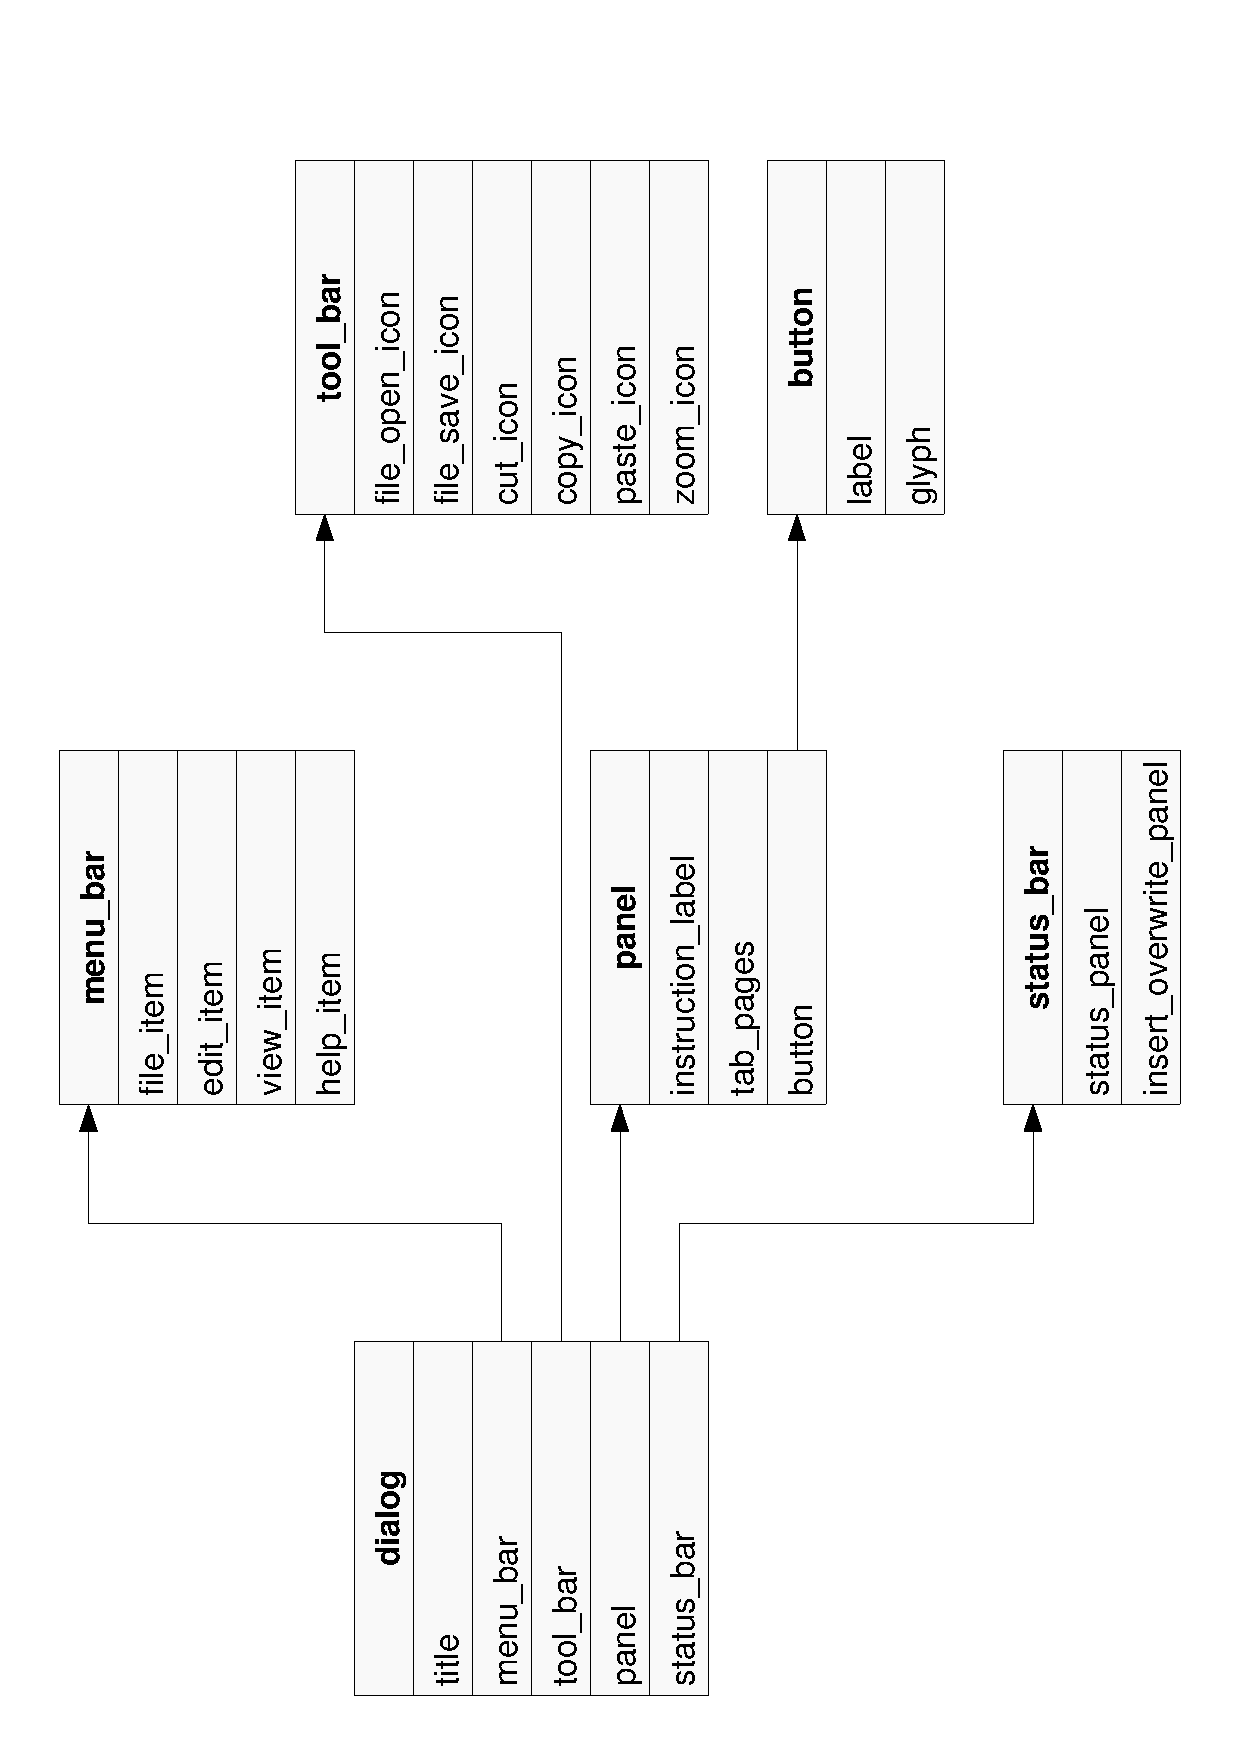
\includegraphics[scale=0.3,angle=-90]{graphics/template_diagram.pdf}
        \caption{CYBOL Template Diagram (TD) Proposal}
        \label{template_diagram_figure}
    \end{center}
\end{figure}

\begin{figure}[ht]
    \begin{center}
        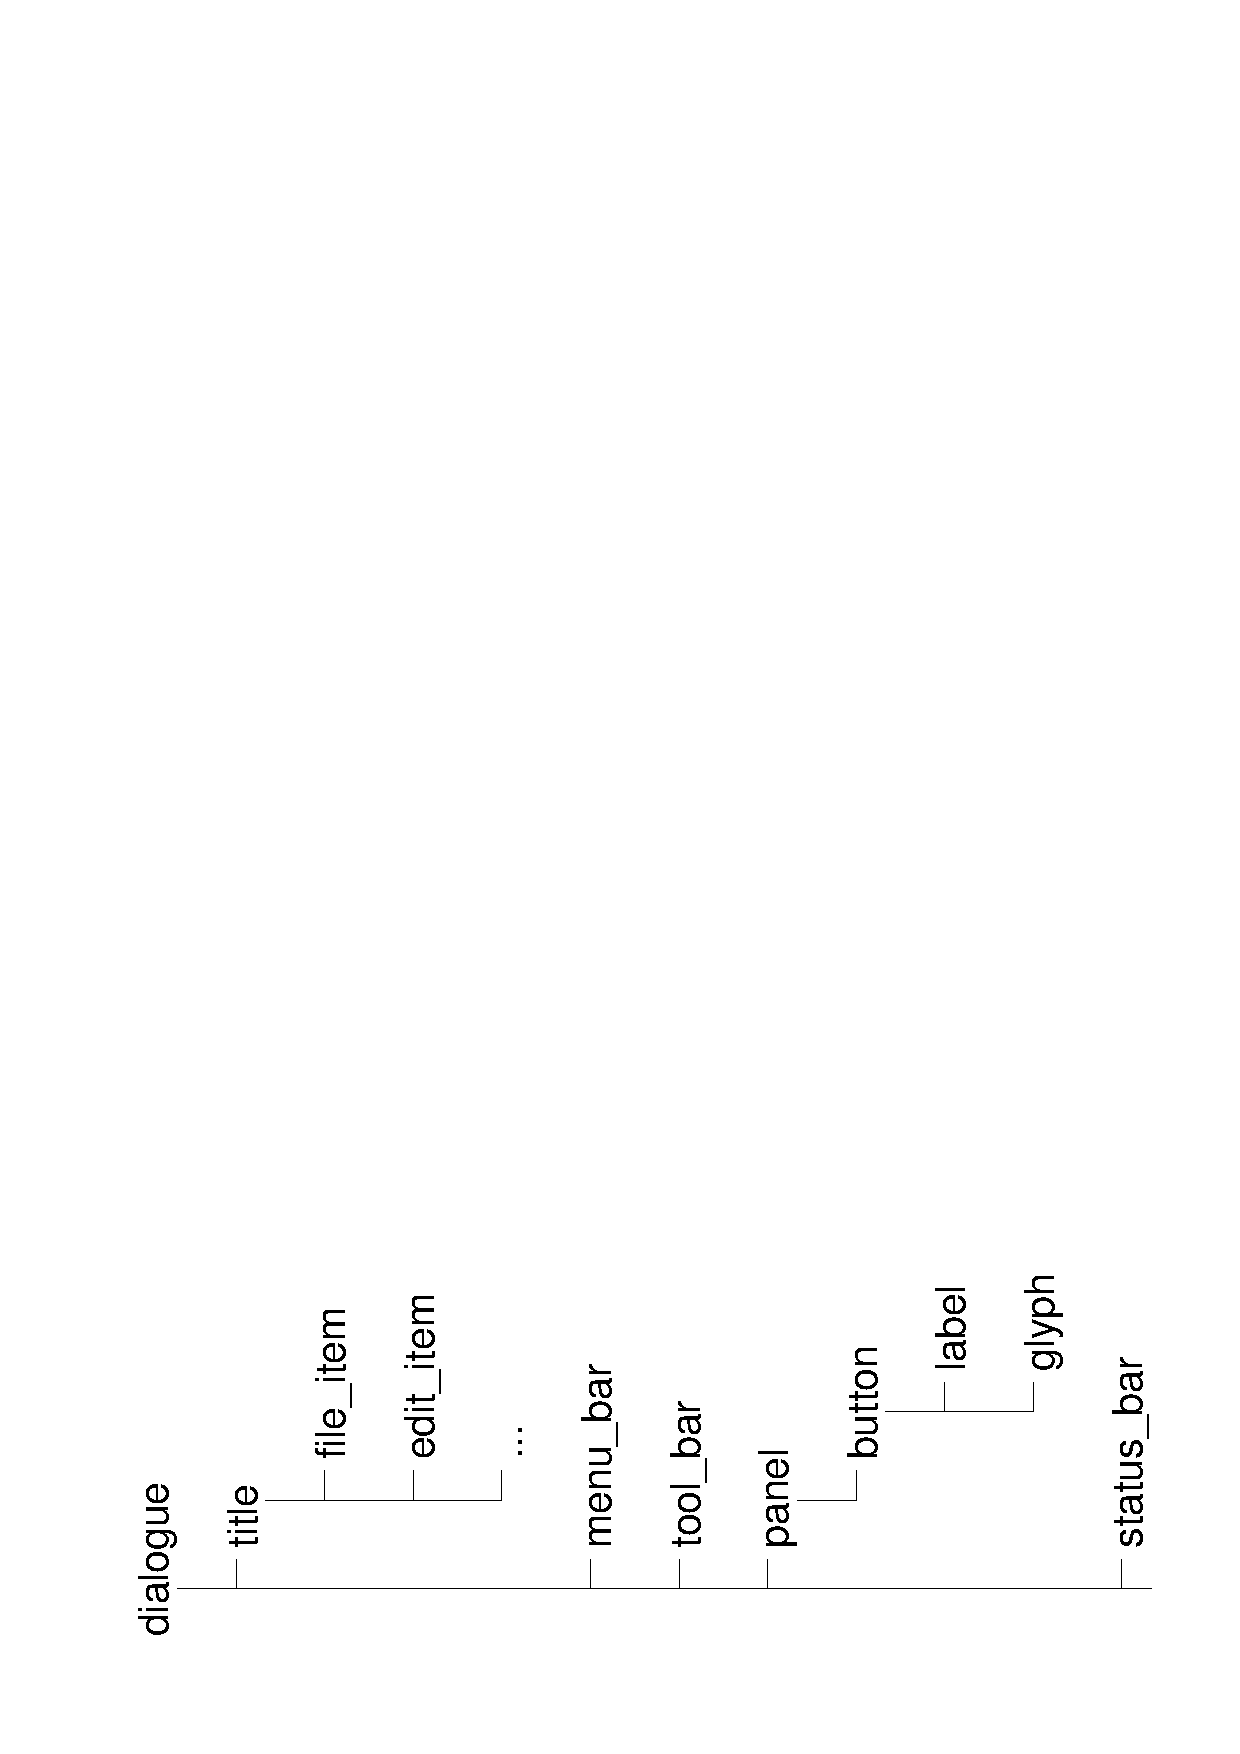
\includegraphics[scale=0.3,angle=-90]{graphics/model_diagram.pdf}
        \caption{CYBOL Model Diagram (MD) Proposal}
        \label{model_diagram_figure}
    \end{center}
\end{figure}

\clearpage

As said above, the four diagrams may look similar to their corresponding UML
pendant. One possible proposal is given for each diagram type. The TD in figure
\ref{template_diagram_figure} illustrates a graphical dialogue. The diagram
looks pretty similar to a UML CsD. Attributes and methods are not bundled in
one concept though, and inheritance does not exist. Associations are drawn if a
concept links to an external concept which may reside in another file (like the
\emph{menu\_bar}), for example. If a part (like the \emph{title}) is hold
inline in the concept, on the other hand, an association is not displayed. Upon
clicking on a part in a concept box, a dialogue opens up that allows the entry
of meta data like the part's channel, abstraction, model and further properties
(details).

The MD in figure \ref{model_diagram_figure} displays the runtime models that were
instantiated with knowledge templates providing the initial values. Again, the
parts of a graphical dialogue were used.

\begin{figure}[ht]
    \begin{center}
        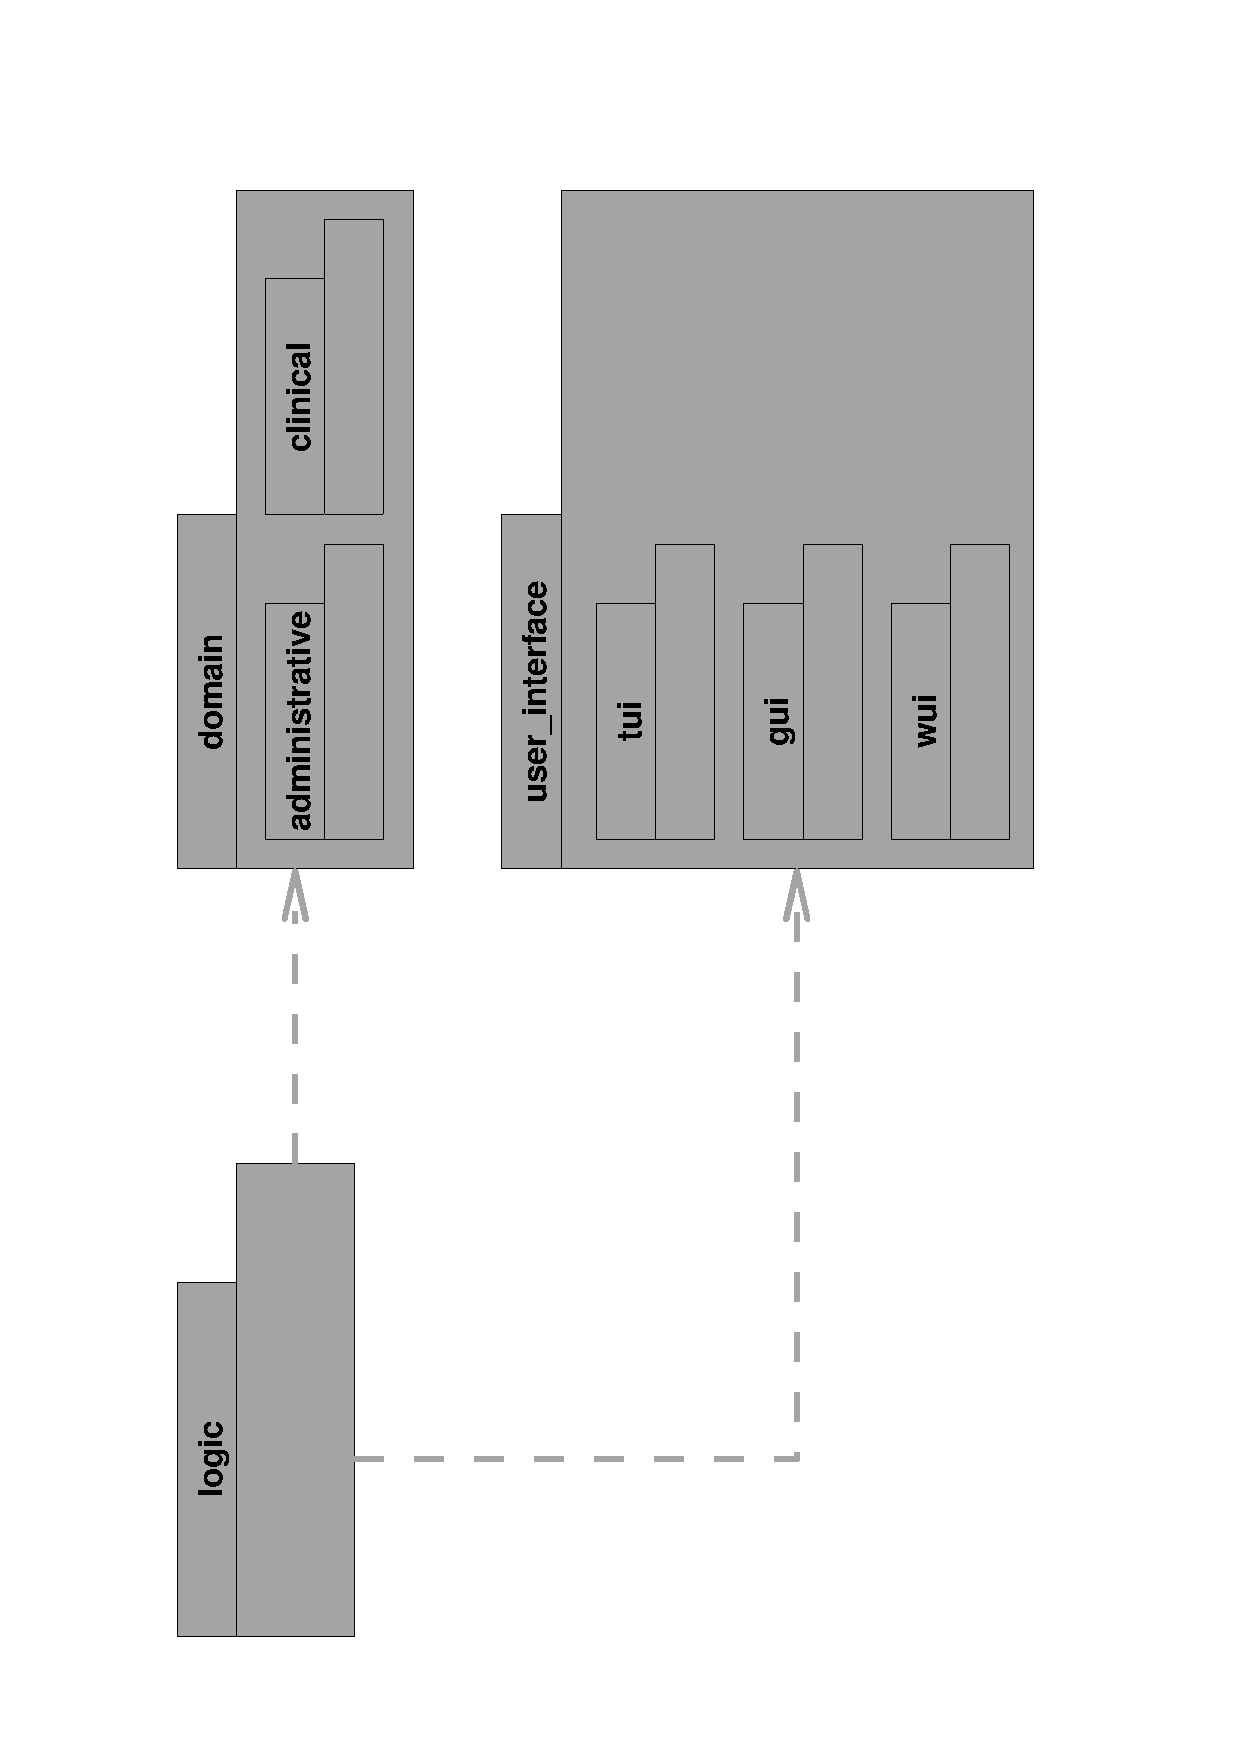
\includegraphics[scale=0.3,angle=-90]{graphics/organisation_diagram.pdf}
        \caption{CYBOL Organisation Diagram (OD) Proposal}
        \label{organisation_diagram_figure}
    \end{center}
\end{figure}

The OD in figure \ref{organisation_diagram_figure} shows packages into which CYBOL knowledge
templates may be organised. Packages do normally correspond to directories on
file system level. The figure contains a \emph{domain} package consisting of
two sub packages, one containing knowledge templates for \emph{administrative}
patient data and the other holding templates for \emph{clinical} data of a
patient. Also, there is a \emph{User Interface} (UI) package containing three
sub packages, for: \emph{Textual UI} (TUI), \emph{Graphical UI} (GUI) and
\emph{Web UI} (WUI). Both, \emph{domain-} as well as \emph{user\_interface}
packages may be accessed from the operations residing in the \emph{logic}
package.

\begin{figure}[ht]
    \begin{center}
        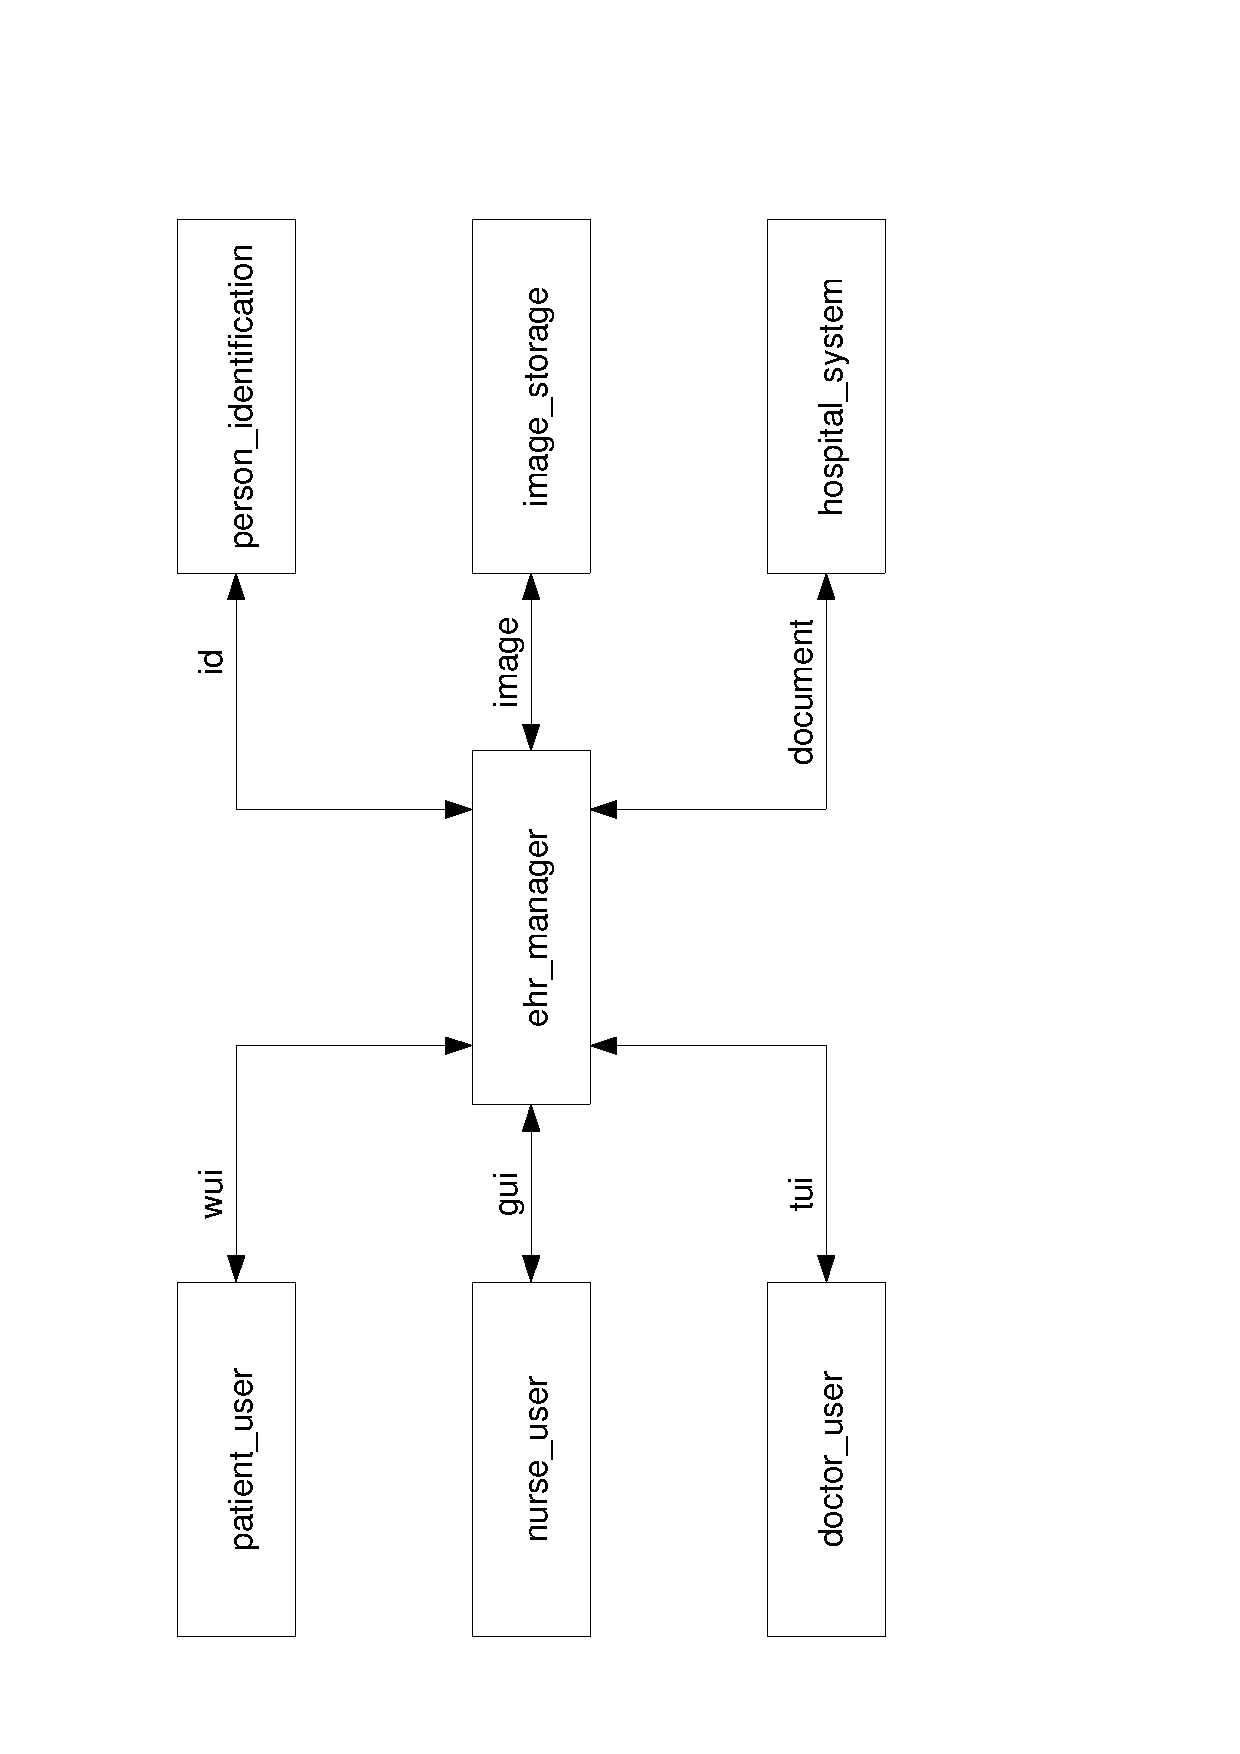
\includegraphics[scale=0.3,angle=-90]{graphics/communication_diagram.pdf}
        \caption{CYBOL Communication Diagram (CD) Proposal}
        \label{communication_diagram_figure}
    \end{center}
\end{figure}

The CD in figure \ref{communication_diagram_figure}, finally, shows a number of independent systems
communicating with each other. An \emph{Electronic Health Record} (EHR) manager
application may be found in the center of the figure. Patients communicate with
it using a WUI; nurses using a GUI and doctors using a TUI (for better
performance). A patient gets identified by asking a \emph{person\_identification}
service. Documents may be exchanged with a \emph{hospital\_system} and images
with a special \emph{image\_storage} system.

    \newpage{\pagestyle{empty}\cleardoublepage}
    %
% $RCSfile: appendices.tex,v $
%
% Copyright (c) 2002-2007. Christian Heller. All rights reserved.
%
% Permission is granted to copy, distribute and/or modify this document
% under the terms of the GNU Free Documentation License, Version 1.1 or
% any later version published by the Free Software Foundation; with no
% Invariant Sections, with no Front-Cover Texts and with no Back-Cover
% Texts. A copy of the license is included in the section entitled
% "GNU Free Documentation License".
%
% http://www.cybop.net
% - Cybernetics Oriented Programming -
%
% Version: $Revision: 1.2 $ $Date: 2007-08-01 13:59:00 $ $Author: christian $
% Authors: Christian Heller <christian.heller@tuxtax.de>
%

\chapter{Appendices}
\label{appendices_heading}

%
% $RCSfile: abbreviations.tex,v $
%
% Copyright (c) 2002-2007. Christian Heller. All rights reserved.
%
% Permission is granted to copy, distribute and/or modify this document
% under the terms of the GNU Free Documentation License, Version 1.1 or
% any later version published by the Free Software Foundation; with no
% Invariant Sections, with no Front-Cover Texts and with no Back-Cover
% Texts. A copy of the license is included in the section entitled
% "GNU Free Documentation License".
%
% http://www.cybop.net
% - Cybernetics Oriented Programming -
%
% Version: $Revision: 1.1 $ $Date: 2007-07-17 20:02:36 $ $Author: christian $
% Authors: Christian Heller <christian.heller@tuxtax.de>
%

%
% More abbreviations can be found at:
%
% http://www.ownnetwork.mfluhr.de/Glossar.htm
% http://www.ciw.uni-karlsruhe.de/abklex.html
% http://www.sans.org/resources/glossary.php
% http://www.cknow.com/ckinfo/acro_d/dde_1.shtml
% http://filext.com/
% http://forum.europa.eu.int/Public/irc/dsis/coded/info/data/abbreviations/en/all.htm
% http://www.sheilapantry.com/figuk/acronyms.html
% http://sir.cyivs.cy.edu.tw/~hchung/computerabbreviation.htm
% http://dmi-www.mc.duke.edu/dukemi/acronyms.htm (healthcare standards)
%

\section[Abbreviations]{Abbreviations}
\label{abbreviations_heading}

\begin{tabbing}
    \hspace{1cm} \= \hspace{2cm} -- \= \hspace{1.5cm}\= \kill

%    \>3GL \>\>Third Generation Language\\

%    \>4GL \>\>Fourth Generation Language\\

%    \>a/c \>\>account\\

%    \>a/o \>\>account of\\

%    \>a/v \>\>ad valorem (according to value)\\

%    \>AAFP \>\>American Academy of Family Physicians\\

%    \>AAP \>\>American Academy of Pediatrics\\

%    \>ABDA \>\>Bundesvereinigung Deutscher Apotheker Verbaende\\

%    \>ACAP \>\>Application Control Access Protocol\\

%    \>ACID \>\>Atomicity, Consistency, Isolation, Durability\\

%    \>ACL \>\>Access Control List\\

%    \>ACL \>\>Agent Communication Language\\

%    \>ACM \>\>Association for Computing Machinery\\

%    \>ACR \>\>American College of Radiology\\

%    \>ad fin. \>\>ad finem\\

%    \>ad inf. \>\>ad infinitem\\

%    \>ad int. \>\>ad interim\\

%    \>ad lib. \>\>ad libitum\\

%    \>ad loc. \>\>ad locum\\

%    \>AD \>\>Activity Diagram\\

%    \>ADA \>\>American Dental Association\\

%    \>ADL \>\>Archetype Definition Language\\

%    \>ADL \>\>Architecture Description Language\\

%    \>ADO \>\>ActiveX Data Object\\

%    \>ADSL \>\>Asymmetrical DSL\\

%    \>ADT \>\>Abrechnungs DT\\

%    \>AE \>\>Application Engineering\\

%    \>AE \>\>Automation Engineering\\

%    \>AGOP \>\>Agent Oriented Programming\\

%    \>AI \>\>Artificial Intelligence\\

%    \>AID \>\>Application ID\\

%    \>AIDS \>\>Anomaly-based IDS\\

%    \>ALU \>\>Arithmetic Logic Unit\\

%    \>AM \>\>Access Mode\\

%    \>AM \>\>Archetype Model\\

%    \>AMA \>\>American Medical Association\\

%    \>AMR \>\>Automated Medical Record\\

%    \>ANN \>\>Artificial Neural Network\\

%    \>ANSI \>\>American National Standards Institute\\

%    \>AODT \>\>Ambulant Operieren DT\\

%    \>AOP \>\>Aspect Oriented Programming\\

%    \>AOSD \>\>Aspect Oriented SD\\

%    \>API \>\>Application Programming Interface\\

%    \>ARP \>\>Address Resolution Protocol\\

%    \>ARQ \>\>Automatic Repeat Request\\

%    \>ARR \>\>Access Rule Reference\\

%    \>ASCII \>\>American Standard Code for Information Interchange\\

%    \>ASD \>\>Adaptive Software Development\\

%    \>ASE \>\>Application Service Element\\

%    \>ASIC \>\>Application Specific IC\\

%    \>ASN \>\>Abstract Syntax Notation\\

%    \>ASP \>\>Active Server Pages\\

%    \>ASP \>\>Application Service Provider\\

%    \>ASTM \>\>American Society for Testing and Materials\\

%    \>AT \>\>AUT Template\\

%    \>ATM \>\>Asynchronous Transfer Mode\\

%    \>ATP \>\>Appletalk Transaction Protocol\\

%    \>ATR \>\>Answer to Reset\\

%    \>AUT \>\>Authentication\\

%    \>AVI \>\>Audio Video Interleave\\

%    \>AWT \>\>Abstract Window Toolkit\\

%    \>B-ISDN \>\>Broadband ISDN\\

%    \>B2B \>\>Business to Business\\

%    \>BASIC \>\>Beginners All purpose Symbolic Instruction Code\\

%    \>B.C. \>\>before Christ\\

%    \>BCD \>\>Binary Coded Decimal\\

%    \>BCDIC \>\>BCD Interchange Code\\

%    \>BDT \>\>Behandlungs DT\\

%    \>BeOS \>\>Be, Inc. OS\\

%    \>BER \>\>Basic Encoding Rules\\

%    \>BIOS \>\>Basic I/O System\\

%    \>Bit \>\>Binary Digit\\

%    \>BLOB \>\>Binary LOB\\

%    \>BMC \>\>BioMed Central\\

%    \>BNF \>\>Backus Naur Form\\

%    \>BO \>\>Business Object\\

%    \>BOOTP \>\>BOOTstrap Protocol\\

%    \>BSD \>\>Berkeley Software (System) Distribution (Design)\\

%    \>C \>\>Certificate\\

%    \>c/o \>\>care of\\

%    \>c/s \>\>client/ server\\

%    \>C.O.D. \>\>Cash on Delivery\\

%    \>CA \>\>Certification Authority\\

%    \>CAD \>\>Computer Aided Design\\

%    \>cADL \>\>Constraint Form of ADL\\

%    \>CAM \>\>Computer Aided Manufacturing\\

%    \>CAP \>\>College of American Pathologists\\

%    \>CAPI \>\>Common ISDN Application Programming Interface\\

%    \>CAR \>\>CA Reference\\

%    \>CASE \>\>Computer Aided Software Engineering\\

%    \>CASE \>\>Common ASE\\

%    \>CBC \>\>Cipher Block Chaining\\

%    \>CBD \>\>Component Based Design (Development)\\

%    \>CBO \>\>Community Based Organisation\\

%    \>CC \>\>Cryptographic Checksum\\

%    \>CCR \>\>Continuity of Care Record\\

%    \>CCT \>\>CC Template\\

%    \>CD \>\>Certificate Directory\\

%    \>CD \>\>Collision Detection\\

%    \>CD \>\>Communication Diagram\\

%    \>CDA \>\>Clinical Document Architecture\\

%    \>CDB \>\>Check Digit Byte\\

%    \>CDDI \>\>Copper Distributed Data Interface\\

%    \>CDISC \>\>Clinical Data Interchange Standards Consortium\\

%    \>CEN \>\>Comite Europeen de Normalisation\\
%        \>\>\>(European Committee for Standardisation)\\

%    \>CENELEC \>\>CEN Electrotechnique\\
%        \>\>\>(European Committee for Electrotechnical Standardisation)\\

%    \>CEO \>\>Chief Executive Officer\\

%    \>CEPT \>\>European Conference of Post and Telecommunication Administrations\\

%    \>CERN \>\>Conseil Europeen pour le Recherche Nucleaire\\

%    \>CertSign \>\>Certificate Signing\\

%    \>CG \>\>Cryptogram\\

%    \>CGI \>\>Common Gateway Interface\\

%    \>CH \>\>Card Holder\\

%    \>CHA \>\>Certificate Holder Authorisation\\

%    \>CHR \>\>Certificate Holder Reference\\

%    \>CIAC \>\>Computer Incident Advisory Capability\\

%    \>CIAS \>\>Clinical Image Access Service\\

%    \>CICS \>\>Customer Information Control System\\

%    \>CII \>\>Computer Implemented Inventions\\

%    \>CIR \>\>Committed Information Rate\\

%    \>CISC \>\>Complex Instruction Set Computing\\

%    \>CL \>\>Common Lisp\\

%    \>CLM \>\>Connectionless Service\\

%    \>CLNP \>\>Connectionless Network Layer Protocol\\

%    \>CLNS \>\>Connectionless Network Service\\

%    \>CLOS \>\>Common Lisp Object System\\

%    \>CLSI \>\>Clinical and Laboratory Standards Institute\\

%    \>CMC \>\>Computer Mediated Communication\\

%    \>CMC \>\>Common Mail Calls\\

%    \>CmD \>\>Component Diagram\\

%    \>CMET \>\>Common Message Element Type\\

%    \>CMM \>\>Capability Maturity Model\\

%    \>CMMI \>\>Capability Maturity Model Integration\\

%    \>CMR \>\>Computerised Medical Record\\

%    \>CMS \>\>Content Management System\\

%    \>CMS \>\>Card Management System\\

%    \>CNS \>\>Central NS\\

%    \>COAS \>\>Clinical Observations Access Service\\

%    \>COBOL \>\>Common Business Oriented Language\\

%    \>CoD \>\>Communication (Collaboration) Diagram\\

%    \>COM \>\>Component Object Model\\

%    \>COM \>\>Connection-Oriented Service\\

%    \>COO \>\>Chief Operating Officer\\

%    \>COP \>\>Component Oriented Programming\\

%    \>CORBA \>\>Common ORB Architecture\\

%    \>COS \>\>Card OS\\

%    \>CP/M \>\>Control Program for Microprocessors\\
%        \>\>\>(Control Program/ Monitor)\\

%    \>CPI \>\>Certificate Profile ID\\

%    \>CPR \>\>Computer-based Patient Record\\
%        \>\>\>(Computerised Patient Record)\\

%    \>CPT \>\>Current Procedural Terminology\\

%    \>CPRI \>\>CPR Institute\\

%    \>CPRS \>\>CPR System\\

%    \>CPU \>\>Central Processing Unit\\

%    \>CR \>\>CEN Report\\

%    \>CRC \>\>Class, Responsibilities, Collaborations\\

%    \>CRC \>\>Cyclic Redundancy Check\\

%    \>CRC \>\>Cyclic Redundancy Code\\

%    \>CRM \>\>Common Reference Model\\

%    \>CS \>\>CertSign\\

%    \>CsD \>\>Class Diagram\\

%    \>CSD \>\>Composite Structure Diagram\\

%    \>CSMA \>\>Carrier Sensing Multiple Access\\

%    \>CSMA/CA \>\>Carrier Sensing Multiple Access with Collision Avoidance\\

%    \>CSMA/CD \>\>Carrier Sensing Multiple Access with Collision Detection\\

%    \>CSP \>\>Certificate Service Provider\\

%    \>CSS \>\>Cascading Style Sheet\\

%    \>CSV \>\>Comma Separated Variable\\

%    \>CT \>\>Computer Tomograph\\

%    \>CTV3 \>\>Clinical Terms Version 3\\

%    \>CVS \>\>Concurrent Versions System\\

%    \>CWA \>\>CEN Working Agreement\\

%    \>CWM \>\>Common Warehouse Metamodel\\

    \>CYBOI \>\>Cybernetics Oriented Interpreter\\

    \>CYBOL \>\>Cybernetics Oriented Language\\

%    \>CYBOM \>\>Cybernetics Oriented Methodology\\

    \>CYBOP \>\>Cybernetics Oriented Programming\\

%    \>CYBORG \>\>Cybernetic Organism\\

%    \>CYBOS \>\>Cybernetics Oriented Operating System\\

%    \>CYBOX \>\>Cybernetics Oriented Box\\

%    \>dADL \>\>Data Definition Form of ADL\\

%    \>DAG \>\>Directed Acyclic Graph\\

%    \>DAML \>\>DARPA Agent ML\\

%    \>DAO \>\>Data Access Object\\

%    \>DARPA \>\>Defense Advanced Research Projects Agency\\

%    \>DB \>\>Database\\

%    \>DB2 \>\>DB 2\\

%    \>DBMS \>\>DB Management System\\

%    \>DCC \>\>Direct Client to Client Protocol\\

%    \>DCD \>\>Document Content Description\\

%    \>DCE \>\>Distributed Computing Environment\\

%    \>DCE \>\>Data Circuit-Terminating Equipment\\
 � �%    \>\>\>(Data Communications Equipment)\\

%    \>DCL \>\>Data Control Language\\

%    \>DCOM \>\>Distributed COM\\

%    \>DD \>\>Deployment Diagram\\

%    \>DDE \>\>Dynamic Data Exchange\\

%    \>DDL \>\>Data Definition Language\\

%    \>DDoS \>\>Distributed Denial of Service\\

%    \>DDP \>\>Datagram Delivery Protocol\\

%    \>DE \>\>Domain Engineering\\

%    \>DEB \>\>Debian GNU/Linux Package\\

%    \>DES \>\>Data Encryption Standard\\

%    \>DFN \>\>Deutsches Forschungsnetz\\

%    \>DHTML \>\>Dynamic HTML\\

%    \>DICOM \>\>Digital Imaging and Communications in Medicine\\

%    \>DIF \>\>Data Interchange Format\\

%    \>DIMDI \>\>Deutsches Institut fuer Medizinische Dokumentation und Information\\

%    \>DIMSE \>\>DICOM Message Service Element\\

%    \>DIN \>\>Deutsches Institut fuer Normung\\

%    \>DIR \>\>Directory\\

%    \>DLC \>\>Dynamic Link Control\\

%    \>DLL \>\>Dynamic Link Library\\

%    \>DML \>\>Data Manipulation Language\\

%    \>DMP \>\>Disease Management Programme\\

%    \>DMR \>\>Digital Medical Record\\

%    \>DNA \>\>Desoxy Ribo Nucleic Acid\\

%    \>DNA \>\>Distributed interNet Application Architecture\\

%    \>DNR \>\>Do Not Resuscitate\\

%    \>DNS \>\>Domain Name Service\\
%        \>\>\>(Domain Name System)\\

%    \>DOM \>\>Document Object Model\\

%    \>DOS \>\>Disk OS\\

%    \>DPMI \>\>DOS Protected Mode Interface\\

%    \>DQDB \>\>Distributed Queue Dual Bus\\

%    \>DSDM \>\>Dynamic System Development Method\\

%    \>DS \>\>Digital Signature\\

%    \>DSI \>\>DS Input\\

%    \>DSL \>\>Digital Subscriber Line\\

%    \>DSL \>\>Domain Specific Language\\

%    \>DSOM \>\>Distributed System Object Model\\

%    \>DSP \>\>Digital Signal Processor\\

%    \>DSSSL \>\>Document Style Semantics and Specification Language\\

%    \>DST \>\>DS Template\\

%    \>DT \>\>Datentraeger\\

%    \>DTD \>\>Document Type Definition\\

%    \>DTE \>\>Data Termination Equipment\\

%    \>DTO \>\>Data Transfer Object\\

%    \>DVI \>\>Device Independent\\

%    \>DVI \>\>Digital Video Interface\\

%    \>e.g. \>\>exempli gratia (for example)\\

%    \>EAA \>\>Enterprise Application Architecture\\

%    \>EBCDIC \>\>Extended BCDIC\\

%    \>EBES \>\>European Board of EDI Standardisation\\

%    \>EBNF \>\>Extended BNF\\

%    \>EC \>\>Existential Conjunctive\\

%    \>ECC \>\>Error Correction Code\\
%        \>\>\>(Error Checking and Correction)\\

%    \>ECML \>\>Electronic Commerce Modeling Language\\

%    \>ED \>\>Emergency Department\\

%    \>EDI \>\>Electronic Data Interchange\\

%    \>EDIF \>\>EDI Format\\

%    \>EDIFACT \>\>EDI for Administration, Commerce and Transport\\

%    \>EDP \>\>Electronic Data Processing\\

%    \>EEG \>\>EBES Expert Group\\

%    \>EEPROM \>\>Electrically Erasable Programmable ROM\\

%    \>EET \>\>Encyclopedia of Educational Technology\\

%    \>EGP \>\>Exterior Gateway Protocol\\

%    \>eHC \>\>Electronic Health Card\\

%    \>EHCR \>\>Electronic Health Care Record\\

%    \>EHR \>\>Electronic Health Record\\

%    \>EHRcom \>\>EHR Communications\\

%    \>EIA \>\>Electronic Industries Alliance\\

%    \>EICAR \>\>European Institute for Computer Anti-Virus Research\\

%    \>EIR \>\>Electronic Insurance Record\\

%    \>EJB \>\>Enterprise Java Bean\\

%    \>EMA \>\>Electronic Messaging Association\\

%    \>EMI \>\>Electronic Medical Infrastructure\\

%    \>EMR \>\>Electronic Medical Record\\

%    \>EN \>\>European Standard\\

%    \>ENV \>\>European Prestandard\\

%    \>EOF \>\>End of File\\

%    \>EPR \>\>Electronic Patient Record\\

%    \>EPS \>\>Encapsulated PS\\

%    \>ER \>\>Endoplasmic Reticulum\\

%    \>ERD \>\>Entity Relationship Diagram\\

%    \>ERM \>\>Entity Relationship Model\\

%    \>ERP \>\>Enterprise Resource Planning\\

%    \>et al. \>\>et alii (and others)\\

%    \>etc. \>\>et cetera (and so on)\\

%    \>ETH \>\>Eidgenoessische Technische Hochschule\\

%    \>ETSI \>\>European Telecommunications Standards Institute\\

%    \>EU \>\>European Union\\

%    \>EUD \>\>End User Development\\

%    \>Extended ML \>\>Extended Meta Language\\

%    \>FAQ \>\>Frequently Asked Question\\

%    \>FAX \>\>Facsimile Transmission\\

%    \>FBO \>\>Faith Based Organisation\\

%    \>FDD \>\>Feature Driven Development\\

%    \>FDDI \>\>Fiber Distributed Data Interface\\

%    \>FDL \>\>Free Documentation License\\

%    \>FeatuRSEB \>\>Feature RSEB\\

%    \>FEC \>\>Forward Error Correction\\

%    \>FHS \>\>Filesystem Hierarchy Standard\\

%    \>FIC \>\>Family of International Classifications\\

%    \>FIFO \>\>First In, First Out\\

%    \>FLOSS \>\>Free/ Libre OSS\\

%    \>FODA \>\>Feature Oriented Domain Analysis\\

%    \>FOLDOC \>\>Free On-line Dictionary of Computing\\

%    \>FOPL \>\>First Order Predicate Logic\\

%    \>FORE \>\>Family Oriented Requirements Engineering\\

%    \>FOSS \>\>Free and OSS\\

%    \>FPGA \>\>Field Programmable Gate Array\\

%    \>FPU \>\>Floating Point Unit\\

%    \>FQN \>\>Fully Qualified Name\\

%    \>FR \>\>Frame Relay\\

%    \>FRAD \>\>FR Access Device\\

%    \>FSF \>\>Free Software Foundation\\

%    \>FTAM \>\>File Transfer, Access and Management\\

%    \>FTP \>\>File Transfer Protocol\\

%    \>GA \>\>Genetic Algorithm\\

%    \>GALEN \>\>Generalised Architecture for Languages,\\
%        \>\>\>Encyclopaedias and Nomenclatures in Medicine\\

%    \>GAN \>\>Global Area Network\\

%    \>GC \>\>Garbage Collector\\

%    \>GCC \>\>GNU�Compiler Collection\\
%        \>\>\>(GNU C�Compiler)\\

%    \>GDI \>\>Graphics Device Interface\\

%    \>GDT \>\>Geraete DT\\

%    \>GEHR \>\>Good European/ EHR\\

%    \>GEMATIK \>\>Gesellschaft fuer Telematikanwendungen der Gesundheitskarte\\

%    \>GGP \>\>Gateway-to-Gateway Protocol\\

%    \>GIF \>\>Graphics Interchange Format\\

%    \>GIMP \>\>General (GNU) Image Manipulation Program\\

%    \>GMDN \>\>Global Medical Device Nomenclature\\

%    \>GNOME \>\>GNU Network Object Model Environment\\

%    \>GNU \>\>GNU is not UNIX\\

%    \>GoF \>\>Gang of Four\\

%    \>GP \>\>Generative Programming\\

%    \>GP \>\>General Practitioner\\

%    \>GPF \>\>General Protection Fault\\

%    \>GPIC \>\>General Purpose Information Component\\

%    \>GPL \>\>General Public License\\

%    \>GPL \>\>General Purpose Language\\

%    \>GPS \>\>Global Positioning System\\

%    \>GRAIL \>\>GALEN Representation and Integration Language\\

%    \>GTK \>\>GIMP Toolkit\\

%    \>GUI \>\>Graphical UI\\

%    \>GUID \>\>Globally Unique ID\\

%    \>h/w \>\>Hardware\\

%    \>HAL \>\>Hardware Abstraction Layer\\

%    \>HBCI \>\>Homenanking Computer Interface\\

%    \>HCI \>\>Human-Computer Interaction\\

%    \>HD \>\>Harmonisation Document\\

%    \>HDD \>\>Hard Disk Drive\\

%    \>HDL \>\>Hardware Description Language\\

%    \>HDLC \>\>High level Data Link Control\\

%    \>HDTF \>\>Healthcare Domain Task Force\\

%    \>HIDS \>\>Host based IDS\\

%    \>HIMSS \>\>Health Information Management and Systems Society\\

%    \>HIPAA \>\>Healthcare Insurance Portability and Accountability Act\\

%    \>HIS \>\>Hospital Information System\\

%    \>HL7 \>\>Health Level Seven\\

%    \>HMVC \>\>Hierarchical MVC\\

%    \>HOWTO \>\>How To? (Subject Specific Help)\\

%    \>HP \>\>Hewlett Packard\\

%    \>HPC \>\>Health Professional Card\\

%    \>HPTC \>\>High Performance Technical Computing\\

%    \>HTML \>\>Hypertext ML\\

%    \>HTTP \>\>Hypertext Transfer Protocol\\

%    \>HTTP-ng \>\>HTTP next generation\\

%    \>HTTPD \>\>HTTP Daemon\\

%    \>HTTPS \>\>HTTP over SSL\\

%    \>HUK \>\>Haftpflicht-Unterstuetzungs-Kasse Coburg\\

%    \>HW \>\>Hardware\\

%    \>HXP \>\>Healthcare Xchange Protocol\\

%    \>i/e \>\>import/ export\\

%    \>i/o \>\>input/ output\\

%    \>i/p \>\>input\\

%    \>IABG \>\>Industrieanlagen-Betriebsgesellschaft\\

%    \>ib. \>\>ibidem (in the same place)\\

%    \>ibid. \>\>ib.\\

%    \>IBM \>\>International Business Machines\\

%    \>i/c \>\>in charge of\\

%    \>IC \>\>Integrated Circuit\\

%    \>ICC \>\>IC Card\\

%    \>ICCSN \>\>ICC SN\\

%    \>ICANN \>\>Internet Corporation for Assigned Names and Numbers\\

%    \>ICD \>\>International Classification of Diseases\\

%    \>ICF \>\>International Classification of Functioning, Disability and Health\\

%    \>ICHI \>\>International Classification of Health Interventions\\

%    \>ICHPPC \>\>International Classification of Health Problems in Primary Care\\

%    \>ICMP \>\>Internet Control Message Protocol\\

%    \>ICN \>\>International Council of Nurses\\

%    \>ICNP \>\>International Classification for Nursing Practice (Procedures)\\

%    \>ICQ \>\>I seek you\\

%    \>ICR \>\>Integrated Care Record\\

%    \>ICPC \>\>International Classification of Primary Care\\

%    \>id. \>\>idem (the same)\\

%    \>ID \>\>Identifier\\

%    \>IDE \>\>Integrated Development Environment\\

%    \>IDEA \>\>International Data Encryption Algorithm\\

%    \>IDL \>\>Interface Definition Language\\

%    \>IDS \>\>Intrusion Detection System\\

%    \>i.e. \>\>id est (that is)\\

%    \>IEEE \>\>Institute of Electrical and Electronics Engineers\\

%    \>IETF \>\>Internet Engineering Task Force\\

%    \>IGMP \>\>Internet Group Management Protocol\\

%    \>IGP \>\>Interior Gateway Protocol\\

%    \>IIIS \>\>International Institute of Informatics and Systemics\\

%    \>IIM \>\>Internet Interaction Management\\

%    \>IIOP \>\>Internet Inter ORB Protocol\\

%    \>IIS \>\>Internet Information Server\\

%    \>IM \>\>Information Model\\

%    \>IMAP \>\>Internet Message Access Protocol\\

%    \>IMP \>\>Interface Message Processor\\

%    \>IMTC \>\>International Multimedia Teleconferencing Consortium\\

%    \>Inc. \>\>Incorporated\\

%    \>InterNIC \>\>Internet Network Information Center\\

%    \>IoC \>\>Inversion of Control\\

%    \>IOD \>\>Interaction Overview Diagram\\

%    \>IOM \>\>Institute of Medicine\\

%    \>IP \>\>Internet Protocol\\

%    \>IPC \>\>Inter-Process Communication\\

%    \>IPv6 \>\>Internet Protocol (Version 6)\\

%    \>IPX \>\>Internet Packet Exchange\\

%    \>IRC \>\>Internet Relay Chat\\

%    \>IRQ \>\>Interrupt Request\\

%    \>IS \>\>International Standard\\

%    \>ISA \>\>Instruction Set Architecture\\

%    \>ISBD \>\>International Standard Book Description\\

%    \>ISDN \>\>Integrated Services Digital Network\\

%    \>ISO \>\>International Organization for Standardization\\

%    \>ISP \>\>Internet Service Provider\\

%    \>IST \>\>Information Science Technology\\

%    \>IT \>\>Information Technology\\

%    \>ITC \>\>MIT Internet \& Telecoms Convergence Consortium\\

%    \>ITU \>\>International Telecommunication Union\\

%    \>J2EE \>\>Java 2 Platform Enterprise Edition\\

%    \>JAR \>\>Java Archive\\

%    \>JDBC \>\>Java DB Connectivity\\

%    \>JDK \>\>Java Development Kit\\

%    \>JEDEC \>\>Joint Electron Device Engineering Council\\

%    \>JFC \>\>Java Foundation Classes\\

%    \>JMS \>\>Java Message Service\\

%    \>JNDI \>\>Java Naming and Directory Interface\\

%    \>JNI \>\>Java Native Interface\\

%    \>JOSMC \>\>Journal of Free and Open Source Medical Computing\\

%    \>JPE \>\>Java Platform for the Enterprise\\

%    \>JPEG \>\>Joint Photographic Experts Group\\

%    \>JPM \>\>Join Point Model\\

%    \>jr. \>\>junior\\

%    \>JSP \>\>Java Server Pages\\

%    \>JTM \>\>Job Transfer and Management (Manipulation)\\

%    \>JTS \>\>Java Transaction Service\\

%    \>JVM \>\>Java VM\\

%    \>KBV \>\>Kassenaerztliche Bundesvereinigung\\

%    \>KDE \>\>K Desktop Environment\\

%    \>KDT \>\>Kommunikations DT\\

%    \>KE \>\>Knowledge Engineering\\

%    \>KE \>\>Key Encipherment\\

%    \>KEI \>\>KE Input\\

%    \>KID \>\>Key ID\\

%    \>KIF \>\>Knowledge Interchange Format\\

%    \>KIS \>\>Krankenhaus Informations System\\

%    \>KMU \>\>Kleines oder Mittelst\"andisches Unternehmen\\

%    \>KQML \>\>Knowledge Query and Manipulation Language\\

%    \>KV \>\>Kassenaerztliche Vereinigung\\

%    \>KVDT \>\>KV DT\\

%    \>l.c. \>\>loco citato (in the place cited)\\

%    \>L2F \>\>Layer 2 Forwarding\\

%    \>L2TP \>\>Layer 2 Tunneling Protocol\\

%    \>LAN \>\>Local Area Network\\

%    \>LAMP \>\>Linux, Apache, MySQL, PHP/ Perl/ Python\\

%    \>LAMPS \>\>LAMP and SSL\\

%    \>LAPB \>\>Link Access Procedure balanced\\

%    \>LAPD \>\>Link Access Procedure D-channel\\

%    \>LAPM \>\>Link Access Procedure for Modems\\

%    \>LaTeX \>\>Lamport TeX\\

%    \>LDAP \>\>Lightweight Directory Access Protocol\\

%    \>LDR \>\>Lifetime Data Repository\\

%    \>LDT \>\>Labor DT\\

%    \>LGPL \>\>Lesser GPL\\

%    \>LIFO \>\>Last In, First Out\\

%    \>LILO \>\>Linux Loader\\

%    \>LLC \>\>Logical Link Control\\

%    \>LOB \>\>Large Object\\

%    \>LOINC \>\>Logical Observation Identifiers, Names and Codes\\

%    \>LQS \>\>Lexicon (Terminology) Query Service\\

%    \>LRC \>\>Longitudinal Redundancy Check\\

%    \>LSB \>\>Least Significant Byte\\

%    \>Ltd. \>\>limited\\

%    \>LTM \>\>Long Term Memory\\

%    \>LUG \>\>Linux User Group\\

%    \>M. Sc. \>\>Master of Science\\

%    \>MAC \>\>Media Access Control\\

%    \>MAN \>\>Metropolitan Area Network\\

%    \>MAPI \>\>Message Application Programming Interface\\

%    \>MAS \>\>Multi Agent System\\

%    \>MathML \>\>Mathematical ML\\

%    \>MATLAB \>\>Matrix Laboratory\\

%    \>MBR \>\>Master Boot Record\\

%    \>MD \>\>Model Diagram\\

%    \>MD \>\>Medical Doctor\\

%    \>MDA \>\>Model Driven Architecture\\

%    \>MDI \>\>Multiple Document Interface\\

%    \>MeSH \>\>Medical Subject Headings\\

%    \>MFC \>\>MS Foundation Classes\\

%    \>MIF \>\>Management Information Format\\

%    \>MIME \>\>Multipurpose Internet Mail Extension\\

%    \>MIS \>\>Management Information System\\

%    \>MIT \>\>Massachusetts Institute of Technology\\

%    \>ML \>\>Markup Language\\

%    \>MMS \>\>Massachusetts Medical Society\\

%    \>MMU \>\>Memory Management Unit\\

%    \>MOF \>\>Meta Object Facility\\

%    \>MOP \>\>Meta Object Protocol\\

%    \>MOTIS \>\>Message-Oriented Text Interchange Systems\\

%    \>MPEG \>\>Moving Picture Experts Group\\
%        \>\>\>(Motion Picture Expert Group)\\

%    \>MPI \>\>Message Passing Interface\\

%    \>MPI \>\>Master Patient Index\\

%    \>MPOA \>\>Multiprotocol over ATM\\

%    \>Mr. \>\>Mister\\

%    \>Mrs. \>\>Mistress\\

%    \>MRPT \>\>Management Resource Planning Tool\\

%    \>MS \>\>Microsoft\\

%    \>MSB \>\>Most Significant Byte\\

%    \>MTP \>\>Message Transfer Protocol\\

%    \>MTU \>\>Maximum Transmission Unit\\

%    \>MUD \>\>Multi User Dungeon\\

%    \>Mutex \>\>Mutual Exclusion\\

%    \>MVC \>\>Model View Controller\\

%    \>MVS \>\>Multiple Virtual Storage\\

%    \>n/a \>\>not applicable\\

%    \>n/a \>\>no account (on cheques)\\

%    \>n.d. \>\>not dated\\

%    \>NAT \>\>Network Adress Translation\\

%    \>NC \>\>Network Computer\\

%    \>NCCLS \>\>National Committee for Clinical Laboratory Standards\\

%    \>NCPDP \>\>National Council for Prescription Drug Programs\\

%    \>NEMA \>\>National Electrical Manufacturers Association\\

%    \>NETBEUI \>\>NetBIOS Extended UI\\

%    \>NetBIOS \>\>Network BIOS\\

%    \>NetDDE \>\>Network DDE\\

%    \>NFS \>\>Network File System\\

%    \>NGI \>\>Next Generation Internet\\

%    \>NGO \>\>Non-Governmental Organisation\\

%    \>NHS \>\>National Health Service\\

%    \>NHSIA \>\>NHS Information Authority\\

%    \>NID \>\>Namespace Identifier\\

%    \>NIDS \>\>Network-based IDS\\

%    \>NIS \>\>Network Information Service\\

%    \>NIST \>\>National Institute of Standards and Technology\\

%    \>NLM \>\>National Library of Medicine\\

%    \>NNTP \>\>Network News Transfer Protocol\\

%    \>NOS \>\>Network OS\\

%    \>NPO \>\>Non-Profit Organisation\\

%    \>NS \>\>Nervous System\\

%    \>NSA \>\>National Security Agency\\

%    \>NSF \>\>National Science Foundation\\

%    \>NSP \>\>Network Service Provider\\

%    \>NSS \>\>Namespace Specific String\\

%    \>NTP \>\>Network Time Protocol\\

%    \>o/a \>\>on account of\\

%    \>o/o \>\>p.c.\\

%    \>o/p \>\>output\\

%    \>OASIS \>\>Organization for the Advancement of Structured Information Standards\\

%    \>ObD \>\>Object (Instance) Diagram\\

%    \>OCL \>\>Object Constraint Language\\

%    \>OCX \>\>OLE Custom Control\\

%    \>OD \>\>Organisation Diagram\\

%    \>ODBC \>\>Open DB Connectivity\\

%    \>ODI \>\>Open Datalink Interface\\

%    \>ODL \>\>Object Description Language\\

%    \>ODM \>\>Operational Data Modeling\\

%    \>ODP \>\>Open Distributed Processing\\

%    \>OFFIS \>\>Oldenburger Forschungs- und Entwicklungsinstitut\\
%        \>\>\>fuer Informatik-Werkzeuge und -Systeme\\

%    \>OGG \>\>Ogg Vorbis Audio Encoding and Streaming Technology\\

%    \>OID \>\>Object ID\\

%    \>OIM \>\>Open Information Model\\

%    \>OIO \>\>Open Infrastructure for Outcomes\\

%    \>OLE \>\>Object Linking and Embedding\\

%    \>OM \>\>Object Model\\

%    \>OMA \>\>Object Management Architecture\\

%    \>OMG \>\>Object Management Group\\

%    \>OMS \>\>Object Model System\\

%    \>OO \>\>Object Oriented\\
%        \>\>\>(Object Orientation)\\

%    \>OOA \>\>OO Analysis\\

%    \>OOD \>\>OO Design\\

%    \>OODBMS \>\>OO DBMS\\

%    \>OOM \>\>OO Model\\

%    \>OOP \>\>OO Programming\\

%    \>OOPS \>\>OO Programming System\\

%    \>OPCS \>\>Office of Population Censuses and Surveys\\
%        \>\>\>Classification of Surgical Operations and Procedures\\

%    \>OPD \>\>Object Process Diagram\\

%    \>OpenEHR \>\>Open EHR\\

%    \>OPS \>\>Official Production System\\

%    \>OQL \>\>Object Query Language\\

%    \>ORB \>\>Object Request Broker\\

%    \>ORDBMS \>\>Object Relational DBMS\\

%    \>OS \>\>Operating System\\

%    \>OSCAR \>\>Open Source Clinical Application Resource\\

%    \>OSDN \>\>Open Source Development Network\\

%    \>OSF \>\>Open Software Foundation\\

%    \>OSHCA \>\>Open Source Health Care Alliance\\

%    \>OSI \>\>Open Source Initiative\\

%    \>OSI \>\>Open Systems Interconnection\\

%    \>OSPF \>\>Open Shortest Path First\\

%    \>OSS \>\>Open Source Software\\

%    \>OTW \>\>Object Technology Workbench\\

%    \>OWiS \>\>Objektorientierte und Wissensbasierte Systeme\\

%    \>OWL \>\>Web Ontology Language\\

%    \>OXMIS \>\>Oxford Medical Information System\\

%    \>p.c. \>\>per cent (%)\\

%    \>P2P \>\>Peer to Peer\\
%        \>\>\>(Person-to-Person, Program-to-Program)\\

%    \>P3P \>\>Platform for Privacy Preferences Project\\

%    \>PACS \>\>Picture Archiving and Communication System\\

%    \>PAD \>\>Protocol Assembler Disassembler\\

%    \>PAN \>\>Personal Area Network\\

%    \>PAP \>\>Password Authentication Protocol\\

%    \>PBM \>\>Packet Based Network\\

%    \>PC \>\>Personal Computer\\

%    \>PCL \>\>Printer Control Language\\

%    \>PCMCIA \>\>PC Memory Card International Association\\

%    \>PCR \>\>Patient Carried Record\\

%    \>PCRF \>\>Patient Care Referral Form\\

%    \>PD \>\>Package Diagram\\

%    \>PDA \>\>Personal Digital Assistant\\

%    \>PDF \>\>Portable Document Format\\

%    \>PDL \>\>Page Description Language\\

%    \>PDU \>\>Protocol Data Unit\\

%    \>PEM \>\>Privacy Enhanced Mail\\

%    \>p.ann. \>\>per annum (yearly)\\

%    \>Perl \>\>Practical Extraction and Report Language\\

%    \>PGP \>\>Pretty Good Privacy\\

%    \>PHAGRO \>\>Bundesverband des pharmazeutischen Groszhandels\\

%    \>PhD \>\>Philosophiae Doctor\\

%    \>PHP \>\>PHP Hypertext Preprocessor\\
%        \>\>\>(Personal Home Page)\\

%    \>PHP \>\>Personal Health Project\\

%    \>PHR \>\>Personal Health Record\\

%    \>PIC \>\>Programmable Interrupt Controller\\

%    \>PICS \>\>Platform for Internet Content Selection\\

%    \>PIDS \>\>Person (Patient) Identification Service\\

%    \>PIM \>\>Platform Independent Model\\

%    \>PIM \>\>Personal Information Manager\\

%    \>PIN \>\>Personal Identification Number\\

%    \>PIO \>\>Programmed Input Output\\

%    \>Pixel \>\>Picture Element\\

%    \>PK \>\>Public Key\\

%    \>PKI \>\>PK Infrastructure\\

%    \>PL/1 \>\>Programming Language One\\

%    \>PLD \>\>Programmable Logic Device\\

%    \>PMR \>\>Patient Medical Record\\

%    \>PMS \>\>Practice Management System\\

%    \>PNG \>\>Portable Network Graphics\\

%    \>PnP \>\>Plug and Play\\

%    \>PNS \>\>Peripheral NS\\

%    \>POA \>\>Portable Object Adapter\\

%    \>POL \>\>Problem Oriented Language\\

%    \>POMR \>\>Problem Oriented Medical Record\\

%    \>POP \>\>Post Office Protocol\\

%    \>POSIX \>\>Portable OS Interface for UNIX\\

%    \>pp. \>\>pages\\

%    \>PPC \>\>Power PC\\

%    \>PPP \>\>Point-to-Point Protocol\\

%    \>PPTP \>\>Point-to-Point Tunneling Protocol\\

%    \>PrK \>\>Private Key\\

%    \>pro tem. \>\>pro tempore (for the time)\\

%    \>Prolog \>\>Programmation en Logique\\

%    \>PS \>\>PostScript\\

%    \>PSM \>\>Platform Specific Model\\

%    \>PURL \>\>Persistent URL\\

%    \>PVC \>\>Permanent Virtual Circuit\\

%    \>q.e. \>\>quod est (which is)\\

%    \>q.e.d. \>\>quod erat demonstrandum (which was to be proved)\\

%    \>q.v. \>\>quod vide (which see)\\

%    \>QMS \>\>Qualitaetsring Medizinische Software\\

%    \>QoS \>\>Quality of Service\\

%    \>Qt \>\>Cute C++ Toolkit\\

%    \>r/t \>\>radio-telegraphy\\

%    \>R.V. \>\>revised version\\

%    \>RAD \>\>Rapid Application Development\\

%    \>RADS \>\>Resource Access Decision Service\\

%    \>RAM \>\>Random Access Memory\\

%    \>RARP \>\>Reverse Address Resolution Protocol\\

%    \>RAS \>\>Remote Access Service\\

%    \>RAS \>\>Reliability, Availability, Serviceability\\

%    \>RDBMS \>\>Relational DBMS\\

%    \>RDF \>\>Resource Description Framework\\

%    \>RDS \>\>Resolver Discovery Service\\

%    \>READ \>\>Read Codes\\

%    \>RF \>\>Radio Frequency\\

%    \>RFC \>\>Request for Comment\\

%    \>RFP \>\>Request for Proposal\\

%    \>RIM \>\>Reference Information Model\\

%    \>RIP \>\>Routing Information Protocol\\

%    \>RIS \>\>Radiology Information System\\

%    \>RISC \>\>Reduced Instruction Set Computing\\

%    \>RKI \>\>Robert Koch Institut\\

%    \>RM \>\>Reference Model\\

%    \>RMI \>\>Remote Method Invocation\\

%    \>RMIM \>\>Refined Message Information Model\\

%    \>RNA \>\>Ribo Nucleic Acid\\

%    \>RND \>\>Random Number\\

%    \>ROM \>\>Read Only Memory\\

%    \>RPC \>\>Remote Procedure Call\\

%    \>RPM \>\>RPM/ Red Hat Package Manager\\

%    \>RSEB \>\>Reuse driven Software Engineering Business\\

%    \>RSP \>\>Resource Reservation Protocol\\

%    \>RSVP \>\>Resource Reservation Setup Protocol\\

%    \>RT \>\>Real Time\\

%    \>RTCP \>\>RT Control Protocol\\

%    \>RTE \>\>Roundtrip Engineering\\

%    \>RTF \>\>Rich Text Format\\

%    \>RTP \>\>RT Protocol\\

%    \>RTTI \>\>Run Time Type Identification\\

%    \>RTZ \>\>Return To Zero\\

%    \>RUP \>\>Rational Unified Process\\

%    \>s.v. \>\>sub voce (under the word)\\

%    \>S/MIME \>\>Secure MIME\\

%    \>s/w \>\>software\\

%    \>SAN \>\>Storage Area Network\\

%    \>SAS \>\>Statistical Analysis System\\

%    \>SANS \>\>System Administration, Networking and Security Institute\\

%    \>SASE \>\>Specific ASE\\

%    \>SAX \>\>Simple API for XML\\

%    \>SC \>\>Subcommittee\\

%    \>SCD \>\>State Chart Diagram\\

%    \>SCDI \>\>Standards Committee on Dental Informatics\\

%    \>SCIPHOX \>\>Standardisation of Communication between Information Systems\\
%        \>\>\>in Physician's Offices and Hospitals using XML\\

%    \>SCN \>\>Switched Circuit Network\\

%    \>SD \>\>Software Development\\

%    \>SD \>\>Sequence Diagram\\

%    \>SDK \>\>System Development Kit\\

%    \>SDL \>\>Specification and Description Language\\

%    \>SDLC \>\>Synchronous Data Link Control\\

%    \>SDM \>\>Submission Data Modeling\\

%    \>SDO \>\>Standards Development Organisation\\

%    \>SDU \>\>Service Data Unit\\

%    \>SEP \>\>Software Engineering Process\\

%    \>SEQUEL \>\>Structured English Query Language\\

%    \>SET \>\>Secure Electronic Transaction\\

%    \>SG \>\>Secretary General\\

%    \>SGB \>\>Sozialgesetzbuch\\

%    \>SGI \>\>Silicon Graphics, Inc.\\

%    \>SGML \>\>Standard Generalized ML\\

%    \>SHTTP \>\>Secure HTTP\\

%    \>SID \>\>Security ID\\

%    \>SIG \>\>Signature\\

%    \>SIG \>\>Special Interest Group\\

%    \>SK \>\>Secret Key\\

%    \>SKA \>\>Sender Keep All\\

%    \>SL \>\>Specification Language\\

%    \>SLIP \>\>Serial Line Internet Protocol\\

%    \>SM \>\>Secure Messaging\\

%    \>SMB \>\>Server Message Block\\

%    \>SMD \>\>State Machine (Chart) Diagram\\

%    \>SME \>\>Small- and Medium Sized Enterprise\\

%    \>SMIF \>\>Stream based Model Interchange Format\\

%    \>SMK \>\>SM Key\\

%    \>SMP \>\>Symmetric Multiprocessing\\
%        \>\>\>(Shared Memory Processing)\\

%    \>SMTP \>\>Simple Mail Transfer Protocol\\

%    \>SN \>\>Serial Number\\

%    \>SNA \>\>Systems Network Architecture\\

%    \>SNAP \>\>SubNetwork Access Protocol\\

%    \>SNMP \>\>Simple Network Management Protocol\\

%    \>SNOMED \>\>Systematized Nomenclature of Medicine\\

%    \>SNOMED CT \>\>SNOMED Clinical Terms\\

%    \>SNOMED RT \>\>SNOMED Reference Terminology\\

%    \>SNR \>\>Signal to Noise Ratio\\

%    \>SOA \>\>Service Oriented Architecture\\

%    \>SOAP \>\>Simple Object Access Protocol\\

%    \>SOAP \>\>Subjective, Objective, Assessment, Plan\\

%    \>SoC \>\>Separation of Concerns\\

%    \>SONET \>\>Synchronous Optical Network\\

%    \>SOP \>\>Script Oriented Programming\\

%    \>SOX \>\>Schema for Object Oriented XML\\

%    \>SPID \>\>Service Profile (Provider) ID\\

%    \>SPL \>\>Special Purpose Language\\

%    \>SPP \>\>Structured and Procedural Programming\\

%    \>SPSS \>\>Statistical Package for the Social Sciences\\

%    \>SPX \>\>Sequence Package Exchange\\

%    \>SQL \>\>Structured Query Language\\

%    \>SR \>\>Search and Retrieve Application Protocol\\

%    \>SS7 \>\>Signaling System 7\\

%    \>SSI \>\>Server Side Include\\

%    \>SSL \>\>Secure Socket Layer\\

%    \>STL \>\>Standard Template Library\\

%    \>STM \>\>Short Term Memory\\

%    \>SVG \>\>Scalable Vector Graphics\\

%    \>SW \>\>Software\\

%    \>SWAN \>\>Storage Wide Area Network\\

%    \>SWIFT \>\>Society for Worldwide Inter-Bank Financial Telecommunication\\

%    \>syn. \>\>synonymous\\

%    \>SynEx \>\>Synergy on the Extranet\\

%    \>SYSOP \>\>System Operator\\

%    \>tADL \>\>Template Form of ADL\\

%    \>TC \>\>Technical Committee\\

%    \>TC \>\>Trusted Channel\\

%    \>TCA \>\>Total Cost of Acquisition\\

%    \>Tcl \>\>Tool command language\\

%    \>TCO \>\>Total Cost of Ownership\\

%    \>TCP \>\>Transfer (Transport, Transmission) Control Protocol\\

%    \>TD \>\>Template Diagram\\

%    \>TEI \>\>Text Encoding Initiative\\

%    \>Telnet \>\>Telephone Network\\

%    \>TFTP \>\>Trivial FTP\\

%    \>TiD \>\>Timing Diagram\\

%    \>TIFF \>\>Tagged Image File Format\\

%    \>Tk \>\>Toolkit\\

%    \>tkFP \>\>Tcl/Tk Family Practice\\

%    \>TLD \>\>Top Level Domain\\

%    \>TLDP \>\>The Linux Documentation Project\\

%    \>TLS \>\>Transport Layer Security\\

%    \>TP4 \>\>Transport Protocol Class 4\\

%    \>TPM \>\>Third Party Maintenance\\

%    \>TR \>\>Technical Report\\

%    \>TS \>\>Technical Specification\\

%    \>TTF \>\>True Type Font\\

%    \>TUG \>\>TeX Users Group\\

%    \>TUI \>\>Technical University of Ilmenau\\

%    \>TUI \>\>Textual UI\\

%    \>TXT \>\>Text\\

%    \>UAP \>\>Unterarbeitspaket\\

%    \>UCAID \>\>University Corporation for Advanced Internet Development\\

%    \>UCD \>\>Use Case Diagram\\

%    \>UDP \>\>User Datagram Protocol\\

%    \>UI \>\>User Interface\\

%    \>UIML \>\>UI ML\\

%    \>UIN \>\>Universal Internet Number\\

%    \>UK \>\>United Kingdom\\

%    \>UMDNS \>\>Universal Medical Device Nomenclature System\\

%    \>UML \>\>Unified Modeling Language\\

%    \>UMLS \>\>Unified Medical Language System\\

%    \>UMLSKS \>\>UMLS Knowledge Source Server\\

%    \>UMTS \>\>Universal Mobile Telecommunications System\\

%    \>UN \>\>United Nations\\

%    \>UNC \>\>Universal Naming Convention\\

%    \>UNICODE \>\>Universal, Unique, Uniform Character Set Standard\\

%    \>UNIX \>\>Universal Interactive Executive\\
%        \>\>\>(Uniplexed Information and Computing System)\\

%    \>UNO \>\>Universal Network Objects\\

%    \>URC \>\>Uniform Resource Characteristics\\

%    \>URI \>\>Uniform Resource Indicator\\

%    \>URIref \>\>URI reference\\

%    \>URL \>\>Uniform Resource Locator\\

%    \>URN \>\>Uniform Resource Name\\

%    \>US \>\>United States\\

%    \>USA \>\>US of America\\

%    \>USB \>\>Universal Serial Bus\\

%    \>USENET \>\>User Network\\

%    \>USR \>\>US Robotics\\

%    \>UUCP \>\>UNIX to UNIX Copy\\

%    \>UUENCODE \>\>UNIX to UNIX Encode\\

%    \>UUID \>\>Universally Unique ID\\

%    \>v. \>\>vid.\\

%    \>v.v. \>\>vice versa (the other way round)\\

%    \>VB \>\>Visual Basic\\

%    \>VC \>\>Virtual Circuit\\

%    \>VCL \>\>Visual Component Library\\

%    \>VDAP \>\>Verband Deutscher Arztpraxis Softwarehersteller\\

%    \>VDDS \>\>Verband Deutscher Dental Software Unternehmen\\

%    \>VDM \>\>Vienna Development Method\\

%    \>VHDL \>\>VHSIC HDL\\

%    \>VHitG \>\>Verband der Hersteller von IT Loesungen fuer das Gesundheitswesen\\

%    \>VHR \>\>Virtual Health Record\\

%    \>VHSIC \>\>Very High Speed IC\\

%    \>vid. \>\>vide (see)\\

%    \>VistA \>\>Veterans Health Information Systems and Technology Architecture\\

%    \>VLAN \>\>Virtual LAN\\

%    \>VM \>\>Virtual Machine\\

%    \>VMM \>\>Virtual Memory Manager\\

%    \>VoIP \>\>Voice over IP\\

%    \>vol. \>\>volume\\

%    \>Voxel \>\>Volume Element\\

%    \>VPN \>\>Virtual Private Network\\

%    \>VPR \>\>Virtual Patient Record\\

%    \>VR \>\>Virtual Reality\\

%    \>VRC \>\>Vertical Redundancy Check\\

%    \>vs. \>\>versus (against)\\

%    \>VSA \>\>Virtual Storage Architecture\\

%    \>VSAM \>\>Virtual Storage Access Method\\

%    \>VTS \>\>Virtual Terminal Service\\

%    \>W3 \>\>WWW\\

%    \>W3C \>\>W3 Consortium\\

%    \>WAIS \>\>Wide Area Information Server\\

%    \>WAN \>\>Wide Area Network\\

%    \>WAP \>\>Wireless Application (Access) Protocol\\

%    \>WAR \>\>Web Archive\\

%    \>WCS \>\>World Coordinate System\\

%    \>WD \>\>Working Document\\

%    \>WG \>\>Working Group\\

%    \>WHO \>\>World Health Organisation\\

%    \>WHOART \>\>WHO Adverse Drug Reaction Terminology\\

%    \>WI \>\>Work Item\\

%    \>WIMP \>\>Windows, Icons, Menus, Pointing\\
%        \>\>\>(Windows, Icons, Mouse, Pull-down Menus)\\

%    \>WINSOCK \>\>Windows Socket\\

%    \>WINTEL \>\>Windows/ Intel\\

%    \>WLAN \>\>Wireless LAN\\

%    \>WLANA \>\>Wireless LAN Alliance\\

%    \>WONCA \>\>World Organization of National Colleges, Academies and Academic Associations of General Practitioners / Family Physicians\\

%    \>WOSA \>\>Windows Open Service Architecture\\

%    \>WUI \>\>Web UI\\

%    \>WWW \>\>World Wide Web\\

%    \>WYSIWYG \>\>What You See Is What You Get\\

%    \>WYSIWYP \>\>What You See Is What You Print\\

%    \>X \>\>X Window System\\

%    \>XAML \>\>Extensible Application ML\\

%    \>xDT \>\>x DT\\

%    \>XHTML \>\>Extensible HTML\\

%    \>Xlibs \>\>X Libraries\\

%    \>XMI \>\>XML Metadata Interchange\\

%    \>XML \>\>Extensible ML\\

%    \>XNS \>\>Xerox Network System\\

%    \>XP \>\>Extreme Programming\\

%    \>XPath \>\>XML Path Language\\

%    \>XSD \>\>XML Schema Definition\\

%    \>XSL \>\>Extensible Stylesheet Language\\

%    \>XSL-FO \>\>XSL Formatting Objects\\

%    \>XSLT \>\>XSL Transformations\\

%    \>XUL \>\>XML UI Language (XUL)\\

%    \>YACC \>\>Yet Another Compiler Compiler\\

%    \>YAHOO \>\>Yet Another Hierarchical Officious Oracle\\

%    \>ZI \>\>Zentralinstitut fuer die Kassenaerztliche Versorgung\\
\end{tabbing}

\newpage{\pagestyle{empty}\cleardoublepage}
\label{references_heading}
\settocbibname{References}
%\bibliographystyle{alpha}
%\bibliographystyle{geralpha}
\bibliographystyle{plain}
%\bibliographystyle{latex8}
\bibliography{references}
\newpage{\pagestyle{empty}\cleardoublepage}
% Unset uppercase for figures and tables headers.
% By default, TeX uses uppercase letters for these.
\lhead[\fancyplain{}{\footnotesize{\textsf{\textsl{\thepage}}}}]{\fancyplain{}{\footnotesize{\textsf{\textsl{\nouppercase{\rightmark}}}}}}
\rhead[\fancyplain{}{\footnotesize{\textsf{\textsl{7\hspace{3mm}Appendices}}}}]{\fancyplain{}{\footnotesize{\textsf{\textsl{\thepage}}}}}
\setlofname{7.3\hspace{3mm}Figures}
% Set sans serif font.
\sffamily
\label{list_of_figures_heading}
\listoffigures
\newpage{\pagestyle{empty}\cleardoublepage}
\setlotname{7.4\hspace{3mm}Tables}
\label{list_of_tables_heading}
\listoftables
% Set roman font.
\rmfamily
\setcounter{section}{4}
\newpage{\pagestyle{empty}\cleardoublepage}
%
% $RCSfile: history.tex,v $
%
% Copyright (C) 2002-2008. Christian Heller.
%
% Permission is granted to copy, distribute and/or modify this document
% under the terms of the GNU Free Documentation License, Version 1.1 or
% any later version published by the Free Software Foundation; with no
% Invariant Sections, with no Front-Cover Texts and with no Back-Cover
% Texts. A copy of the license is included in the section entitled
% "GNU Free Documentation License".
%
% http://www.cybop.net
% - Cybernetics Oriented Programming -
%
% http://www.resmedicinae.org
% - Information in Medicine -
%
% Version: $Revision: 1.3 $ $Date: 2009-02-07 00:39:21 $ $Author: christian $
% Authors: Christian Heller <christian.heller@tuxtax.de>
%

\section{History}
\label{history_heading}

For those who are interested in how I came to develop the concepts introduced
in this book, I have created this small history of events and enlightening ideas.

\begin{itemize}
    \item[1986] Although having difficulties, my father manages to cross the
        border to West-Germany by visiting some relatives. He also manages to
        come back into the East :-) and a present I get is a brand-new
        \emph{Commodore 64} home computer. I mostly play games on it but also
        do my first steps in programming with \emph{BASIC}.
    \item[1988] In the late days of East Germany, new computer subjects are
        introduced at schools. So I take part in them and continue learning
        \emph{BASIC} and some \emph{dBASE}.
    \item[1990] At the \emph{Technical University of Ilmenau}, one of the first
        subjects in my study is \emph{Algorithms and Programming} where we learn
        structural programming in \emph{Turbo Pascal}.
    \item[1993] During my year abroad at \emph{Sussex University} in Brighton,
        England, I come in touch with the \emph{Internet} (email) and
        \emph{UNIX machines}.
    \item[1994] Back in Germany, I start \emph{administrating} the information
        infrastructure in my parents' medical practice, learn about
        \emph{Computer Hardware} and wonder about how doctors are cheated with
        overpriced products and services.
    \item[1995] In the German \emph{c't} computer magazine, I develop an
        announcement of a new operating system called \emph{Linux}. I order and
        install my first distribution, \emph{SuSE November 1995}.
    \item[1995] We have a quite theoretical lecture on
        \emph{Object Oriented Programming} in \emph{Smalltalk}. However, that
        is the first time I hear about those (then still new) programming
        concepts.
    \item[1996] During my student's research project and diploma work, I
        implement parts of a \emph{Neural Network} in \emph{Object Pascal}
        (Delphi).
    \item[1998] First steps in \emph{C++} at my first employer
        \emph{HM Informatics}.
    \item[1999] At \emph{OWiS Software}, I learn to change my thinking away
        from only the source code -- towards the actual \emph{Concepts} and
        \emph{Architecture} behind a software. I also learn how to use the
        \emph{Unified Modeling Language} (UML).
    \item[2000] Recognising the opening of the \emph{SourceForge} developer
        portal in 1999, I set up the \emph{Res Medicinae} project in April 2000.
        It aims at creating a \emph{Medical Software} for physicians.
        Preparation, website, investigation on similar projects and so on take
        months.
    \item[2000] My \emph{Java} knowledge can be manifested at
        \emph{Intershop Communications} where we are building solutions for
        e-commerce (Web Client-Server Applications).
    \item[2001] I visit my first \emph{Free and Open Source Software Developers'
        Meeting} (FOSDEM) in Brussels, Belgium, where Richard M. Stallman of
        the \emph{Free Software Foundation} (GNU project) holds a talk.
    \item[2001] Returned to my former university, I start active coding on
        \emph{Res Medicinae} in April 2001. It takes some time to handle the
        \emph{Concurrent Versions System} (CVS).
    \item[2001] Following the standard approach and several Java Tutorials,
        my first application is nothing more than a \emph{main} method which
        creates a Java Swing \emph{JFrame}.
    \item[2001] Stepwise, I start moving out code into special classes, like
        for example all \emph{GUI} code into a class \emph{Frame}.
    \item[2001] Soon I loose overview and realise the need for some clearer
        structure. I remember the \emph{Design Patterns} applied at my former
        employers and start using the \emph{Model View Controller} (MVC) and
        further patterns.
    \item[2001] Since flexibility is one of the most important aims of my
        efforts, I realise the shortcomings of \emph{MVC} and the
        \emph{Observer} pattern (bidirectional dependencies), especially when
        it comes to web applications. A good solution I find is the
        \emph{Hierarchical Model View Controller} (HMVC) design pattern,
        applied by the \emph{Scope} free software project.
    \item[2002] My disposedness to style guides, clean and well-documented code
        lets me structure and order every method and attribute and check them
        all for \emph{NULL} pointer errors and other exceptions. I find out
        that every attribute not only needs a \emph{set} and \emph{get} method,
        but also a \emph{create} and \emph{destroy} method. Class names as type
        information are handed over to the create method in form of a string.
    \item[2002] Following the idea of \emph{create} and \emph{destroy} methods,
        I come across the \emph{Component Lifecycle}, described by the
        \emph{Apache-Jakarta} project. I change all code by applying
        \emph{Lifecycle Methods}.
    \item[2002] Having read the \emph{OpenEHR Design Document}, I know that
        classes should be grouped in layers with clear dependencies, called an
        \emph{Ontology}. Higher-layer objects consist of objects from lower-level
        layers, but not the other way. I restructure my code by moving all
        classes into new packages (directories), each representing an
        \emph{Ontological Level}.
    \item[2002] Apache's lifecycle \emph{Concerns} turn out to be useless. They
        only break the ontology rack and violate its dependency rules by
        connecting otherwise strictly separated system parts. Moreover, concerns
        encourage the inheritance of redundant or overlapping properties. The
        same counts for variations like \emph{Aspects} and \emph{Interfaces} in
        general. I replace them all by pure \emph{Classes}, following the
        ontology structure.
    \item[2002] I begin to realise that not only \emph{View} (MVC) and
        \emph{Controller} (HMVC) are \emph{hierarchical}, but also the
        \emph{Model} (Knowledge/ Domain) is. In many days and weeks of intensive
        thinking I find that -- as in Universe -- actually \emph{every} other
        software component is hierarchical, too. Consequently, I introduce one
        top-most super (meta) class \emph{Item} that represents a simple
        \emph{Tree} (\emph{Map} container). Inheriting classes do not need to
        implement \emph{create}, \emph{destroy}, \emph{set} or \emph{get}
        methods any longer since they inherit them from \emph{Item}. This saves
        me hundreds of lines of code, at once, and improves clearness a lot.
\end{itemize}

And this is my personal \textbf{Break-Through}. From now on, I first think
about nature and its concepts and then implement software source code.
Suddenly, everything seems easier, I have an \emph{Example}, a
\emph{Way-to-go}: \emph{Nature}. There aren't less (rather more) tasks to solve
now, but at least the direction is clear.

\begin{itemize}
    \item[2002] By applying the new concepts, one difference gets very clear:
        \emph{System Control-} and \emph{Domain Model} code are both
        hierarchical, but different ontologies need to be defined for them.
        An \emph{active} system works on a \emph{passive} model, that is it
        depends on it. While a system provides the means for \emph{input} and
        \emph{output} and \emph{controls} the \emph{Action} (\emph{Workflow}),
        a model just represents domain data. Searching for parallels in nature,
        I find that \emph{Human Body} and \emph{Human Brain} correspond to
        \emph{System} and \emph{Model}. What humans (possibly unconsciously)
        want to do is to imitate themselves, with robots as with computers as
        with other machines, tools or abstractions.
    \item[2002] The overall structure of the \emph{Framework} seems clear now.
        There will be three major parts, \emph{Basic}, \emph{Model} and
        \emph{System}. \emph{Model} and \emph{System} both depend on the
        fundamental abstractions of the \emph{Basic} package which encapsulates
        programming language types. In addition, \emph{System} depends on
        \emph{Model}.
    \item[2003] Encountering difficulties in synchronising \emph{Frontend} and
        \emph{Backend}, I come to the conclusion that they are actually the
        same, passive data models that have to be translated into each other.
        It is not necessary -- even badly wrong -- to apply different design
        patterns for their implementation. I change inheritances and
        dependencies of many of my framework classes so that finally
        \emph{Knowledge-}/ \emph{Domain-}, \emph{Backend-}, \emph{Communication-}
        and \emph{Frontend} models are of the same super type. This decision
        opens unforeseen new possibilities. All kinds of frontends, all
        communication and backend mechanisms can now be implemented
        \emph{modular} and \emph{flexible}.
    \item[2003] Java's event handling using \emph{ActionListener} interfaces
        ignores the dependencies between ontological layers and is thus improper
        (just like the concern interfaces mentioned above). I implement a new
        \emph{Signal Handling} mechanism which is oriented on parts of a
        sentence in human language like \emph{Subject}, \emph{Predicate},
        \emph{Object}.
    \item[2003] I realise how far I have moved away from my original aim of
        writing a small medical application. While implementing the new signal
        handling mechanism it gets clear that I move more and more towards the
        operating system and its hardware input/ output handling code which
        scares me a bit. But there seems to be no other way to go when aiming
        at the creation of clear, easy, modular, flexible, correct systems.
    \item[2003] \emph{Exceptions} are system-internal \emph{Signals}. It is not
        necessary to use an extra signalling mechanism for exception handling.
        And it is dangerous for security if an instance knows about its parent
        to bubble up an exception. For now, I remove all exceptions besides the
        standard one, which again saves me many lines of unnecessary code.
    \item[2003] An abstract model has multiple properties. Not only it keeps
        references to its parts (attributes) and procedures (methods), but also
        it knows about the \emph{Model} and \emph{Position} (and possibly more
        \emph{Meta} properties) of each part.
    \item[2003] After difficulties with the item meta model, I realise that I
        actually want to replace the standard \emph{Class Concept} offered by
        Java and other Object Oriented languages. It takes me some weeks of
        thinking to find the reason and way out: Traditional programming mixes
        \emph{Knowledge} with the \emph{Handling} of its instances. Both need
        to be separated. I move most classes to XML-based \emph{Model} files and
        call their specification \emph{Cybernetics Oriented Language} (CYBOL).
\end{itemize}

Here begins a \emph{New Era}. From now on, business domain \emph{Knowledge}
and hardware-close \emph{System Control} code are stored separately and treated
differently. The concepts to store \emph{static} knowledge are very different
from those that are used to \emph{dynamically} control a system's hardware.

\begin{itemize}
    \item[2003] Later comparisons with biology support my theory. The genetic
        information is static knowledge that gets forwarded from one cell to
        another, during \emph{Cell Separation}. The dynamic processing of that
        knowledge, that is the creation and functioning of organelles is a
        completely different issue. In a similar manner, application knowledge
        has to become transportable between different platforms and absolutely
        independent from hardware.
    \item[2003] Since the time when I first experimented with lifecycle methods
        \`a la \emph{Apache Jakarta}, I had used a \emph{configure} method in
        my code which could read external configuration files and configure
        internal items accordingly. Nothing different was needed to read CYBOL
        files. They represented the whole application configuration knowledge
        and only had to be interpreted correctly. The remaining Java code
        therefore not only had to contain system control functionality, but
        also had to be able to read and write knowledge in form of CYBOL files.
        For that reason, it was called \emph{Cybernetics Oriented Interpreter}
        (CYBOI).
    \item[2003] In search for new concepts and ideas, I also read about a
        number of philosophical theories from Aristotle, Leibnitz and others
        and can identify a mistake in my thinking: the important separation is
        not between \emph{Body} and \emph{Brain} as presumed before, it is
        between \emph{Body/Brain} and \emph{Mind}! \emph{Neural Networks} try
        to imitate the functioning of the physical brain, but what I wanted to
        do is to imitate concepts of the logical mind, of human thinking.
    \item[2003] Reading a magazine about psychology and neurology, I come to
        reflect the principles of \emph{Human Thinking}. I see parallels to
        basic concepts of software modelling and try to connect them. As result,
        I can identify three fundamental kinds of abstraction that our brain
        uses to understand its real-world environment: \emph{Discrimination},
        \emph{Categorisation} and \emph{Composition}. Software developers apply
        these concepts all the time.
    \item[2003] From previous reflections I recall that a \emph{Whole} item
        knows about the properties of its \emph{Part} items. I try to identify
        such meta properties, read about \emph{Shape}, \emph{Depth},
        \emph{Movement} as well as \emph{Colour} in my Psychology literature
        and finally stumble about \emph{Dimensions} as known from physics. The
        position and extension that part items span up within their whole item
        do not only exist in \emph{Space} and \emph{Time}, but possibly also in
        other kinds of dimensions like \emph{Mass} or \emph{Force}.
    \item[2003] Since CYBOL contains all concepts that are necessary to model
        knowledge, including \emph{Categorisation} (inheritance), a CYBOI written
        in \emph{Java} causes unnecessary overhead. The interpreter's main tasks
        (input/ output- and memory handling as well as processing instructions)
        are anyway situated close to hardware so that I start to reimplement
        CYBOI in the \emph{C} programming language.
    \item[2004] An open problem that had caused me many headaches was the
        handling of instructions. I remember the unification of communication
        models which represented \emph{States} that could be transformed into
        each other by help of \emph{Translators}. Journeys into
        \emph{Systems Theory} and a consideration of the \emph{Black Box}
        concept show the solution: \emph{State} and \emph{Logic} knowledge need
        to be separated! The logic contains the rules (algorithms, operations)
        after which an input state is translated into an output state. It takes
        considerable thinking to figure out a common CYBOL structure capable of
        representing states as well as logic.
    \item[2004] The early CYBOL definition turns out to be insufficient. In hot
        but constructive discussions with Rolf Holzmueller, one of my students,
        the reason gets clearer and clearer to me: CYBOL must consider \emph{two}
        different hierarchies in just \emph{one} model. One \emph{Model Hierarchy}
        represents the compound model as such. A second \emph{Meta Hierarchy}
        holds meta information that a \emph{Whole} knows about its \emph{Parts}.
        The old CYBOL tried to put everything into XML attributes. The new CYBOL
        uses XML attributes to link to parts and XML tags to model meta
        information such as \emph{Properties} and \emph{Constraints}.
    \item[2004] A lot of time goes into the implementation of CYBOI. Techniques
        that have to be considered are, among others: signalling, threads,
        UNIX and TCP/IP sockets.
    \item[2005] While implementing a CYBOL prototype application, standard
        programming constructs such as for \emph{Branching} and \emph{Looping}
        are badly missing. It takes some reflexion to decompose these into
        their actual elements and to provide the corresponding CYBOL operations
        by using simple flags.
    \item[2005] A further problem is the automatic indexing of \emph{Parts}
        belonging to a common list within a \emph{Whole} model, for which a
        special \emph{Name Structure} has to be defined and additional CYBOI
        routines have to be written.
    \item[2005] It turns out to be problematic to use existing
        \emph{Graphical User Interface} (GUI) frameworks for input/ output
        (i/o). Many of them base on OOP principles; all require the adoption of
        special structures. Since the first version of CYBOI is developed under
        the \emph{Linux} \emph{Operating System} (OS), low-level
        \emph{X Window System Libraries} (Xlibs) functions are used instead of
        a toolkit.
    \item[2005] The reception of signals (input) is moved into special threads,
        one for graphical-, one for textual user interfaces, one for sockets
        etc. But how can CYBOI handle these signals, if it has no application
        knowledge? The solution is to, as property of the \emph{receive}
        operation, hand over a node of the knowledge tree containing possible
        commands to react to, which are mapped to their corresponding handler
        operations, in CYBOL.
    \item[2005] The CYBOP theory is handed in as dissertation thesis.
\end{itemize}

The \emph{Theoretical Basis} seems pretty clear now. Future work will focus
on the architecture and implementation of the \emph{CYBOI Interpreter}.

\begin{itemize}
    \item[2006] Within two months of being unemployed, I review the CYBOI
        implementation of input/ output (i/o) threads, and can correct open
        conflicts by using \emph{Mutual Exclusion} (Mutex) flags.
        Also, \emph{Central Processing Unit} (CPU) busy states are now avoided.
    \item[2006] Branches of the runtime knowledge tree are pointed to in CYBOL
        by dot-separated names. Since sometimes, it is necessary to address meta
        information (such as the colour of a menu item) directly, the knowledge
        path gets extended by a second separation character, which allows to
        distinguish between whole-part and meta elements.
    \item[2007] The CYBOP theory is published in form of a book.
    \item[2008] One mistake leading to conflicts with CYBOI memory handling was
        that too much functionality had been put into the thread functions,
        e.g. the handling of a signal, reception and conversion of data.
        All that is now done in the main thread instead. What remains for the
        input/ output threads is just the setting of an interrupt flag in a
        "sense" function, whenever data arrive.
    \item[2008] All CYBOI source code gets adapted to using wide characters/ Unicode.
    \item[2008] CYBOL abstraction constants now follow the MIME type schema.
        All constants, no matter for which kind of model or format,
        get categorised into "abstraction", "channel", "model", "name".
        This was not easy to figure out, since at the beginning,
        it was not obvious to me that all kinds of formats (xdt, html etc.)
        and even composed primitive structures (fraction, complex etc.):
        use some kind of name/ index/ key/ identification to identify the parts;
        know about the abstraction/ type of their parts (even a file system knows
        about whether it deals with a directory or file, and which kind of file);
        contain the actual model/ data/ value.
    \item[2009] Various converters get implemented, e.g.:
        xml, tcp socket, http request/ response, uri, html.
    \item[2010] Array functions are unified for all primitive data types.
    \item[2011] The whole container framework gets refactored and simplified.
        It is based on three fundamental structures: array, item, part.
        The former compound structure is now just a simple pointer array
        holding references to parts.
    \item[20xx] Open issues yet to be implemented are, for example:
        compiling CYBOI under \emph{Windows} OS and making use of their GUI
        functionality; improving the GUI layout and providing a GUI theme
        infrastructure; specifying serialisation in more detail.
        For further tasks, see section \ref{call_for_developers_heading}!
\end{itemize}

\newpage{\pagestyle{empty}\cleardoublepage}
%
% $RCSfile: licences.tex,v $
%
% Copyright (c) 2002-2007. Christian Heller. All rights reserved.
%
% Permission is granted to copy, distribute and/or modify this document
% under the terms of the GNU Free Documentation License, Version 1.1 or
% any later version published by the Free Software Foundation; with no
% Invariant Sections, with no Front-Cover Texts and with no Back-Cover
% Texts. A copy of the license is included in the section entitled
% "GNU Free Documentation License".
%
% http://www.cybop.net
% - Cybernetics Oriented Programming -
%
% Version: $Revision: 1.2 $ $Date: 2007-08-01 13:59:00 $ $Author: christian $
% Authors: Christian Heller <christian.heller@tuxtax.de>
%

\section{Licences}
\label{licences_heading}

\input{general_public_license}
\newpage{\pagestyle{empty}\cleardoublepage}
\input{free_documentation_license}

\newpage{\pagestyle{empty}\cleardoublepage}
% Set sans serif font.
\sffamily
\setindexname{Index}
\label{index_heading}
% Include sorted index.
\printindex

\end{document}

%
% $RCSfile$
%
% Copyright (c) 2005-2006. Christian Heller. All rights reserved.
%
% Permission is granted to copy, distribute and/or modify this document
% under the terms of the GNU Free Documentation License, Version 1.1 or
% any later version published by the Free Software Foundation; with no
% Invariant Sections, with no Front-Cover Texts and with no Back-Cover
% Texts. A copy of the license is included in the section entitled
% "GNU Free Documentation License".
%
% http://www.cybop.net
% - Cybernetics Oriented Programming -
%
% http://www.resmedicinae.org
% - Information in Medicine -
%
% Version: $Revision$ $Date$ $Author$
% Authors: Christian Heller <christian.heller@tuxtax.de>
%

\subsection{CYBOI}
\label{cyboi_heading}

The pure existence of proper knowledge does not suffice to create an improved
kind of software system, within a slimmer software development process. The
system needs to know how to \emph{handle} knowledge, at runtime. The criticism
is twofold, since traditionally:

\begin{enumerate}
    \item Operating systems don't have sufficient knowledge handling capabilities
    \item Applications contain too much low-level system control functionality
\end{enumerate}

This is changed when using CYBOI. As active interpreter encapsulating
system-level functionality, it handles knowledge provided in form of passive
CYBOL templates. In CYBOP systems, all compound knowledge models have the same
type structure (schema). Since they do not differ, they can be manipulated in
the same manner.

%
% $RCSfile$
%
% Copyright (c) 2005-2006. Christian Heller. All rights reserved.
%
% Permission is granted to copy, distribute and/or modify this document
% under the terms of the GNU Free Documentation License, Version 1.1 or
% any later version published by the Free Software Foundation; with no
% Invariant Sections, with no Front-Cover Texts and with no Back-Cover
% Texts. A copy of the license is included in the section entitled
% "GNU Free Documentation License".
%
% http://www.cybop.net
% - Cybernetics Oriented Programming -
%
% http://www.resmedicinae.org
% - Information in Medicine -
%
% Version: $Revision$ $Date$ $Author$
% Authors: Christian Heller <christian.heller@tuxtax.de>
%

\subsubsection{Overall Placement}
\label{overall_placement_heading}

Considering an overall computer system architecture, \emph{CYBOI} is situated
between the application knowledge existing in form of \emph{CYBOL} templates
and the \emph{Hardware} controlled by an \emph{Operating System} (OS) (figure
\ref{connection_figure}). CYBOI can thus also be called a
\emph{Knowledge-Hardware-Interface} (synonymous with \emph{Mind-Brain-Interface}).

\begin{figure}[ht]
    \begin{center}
        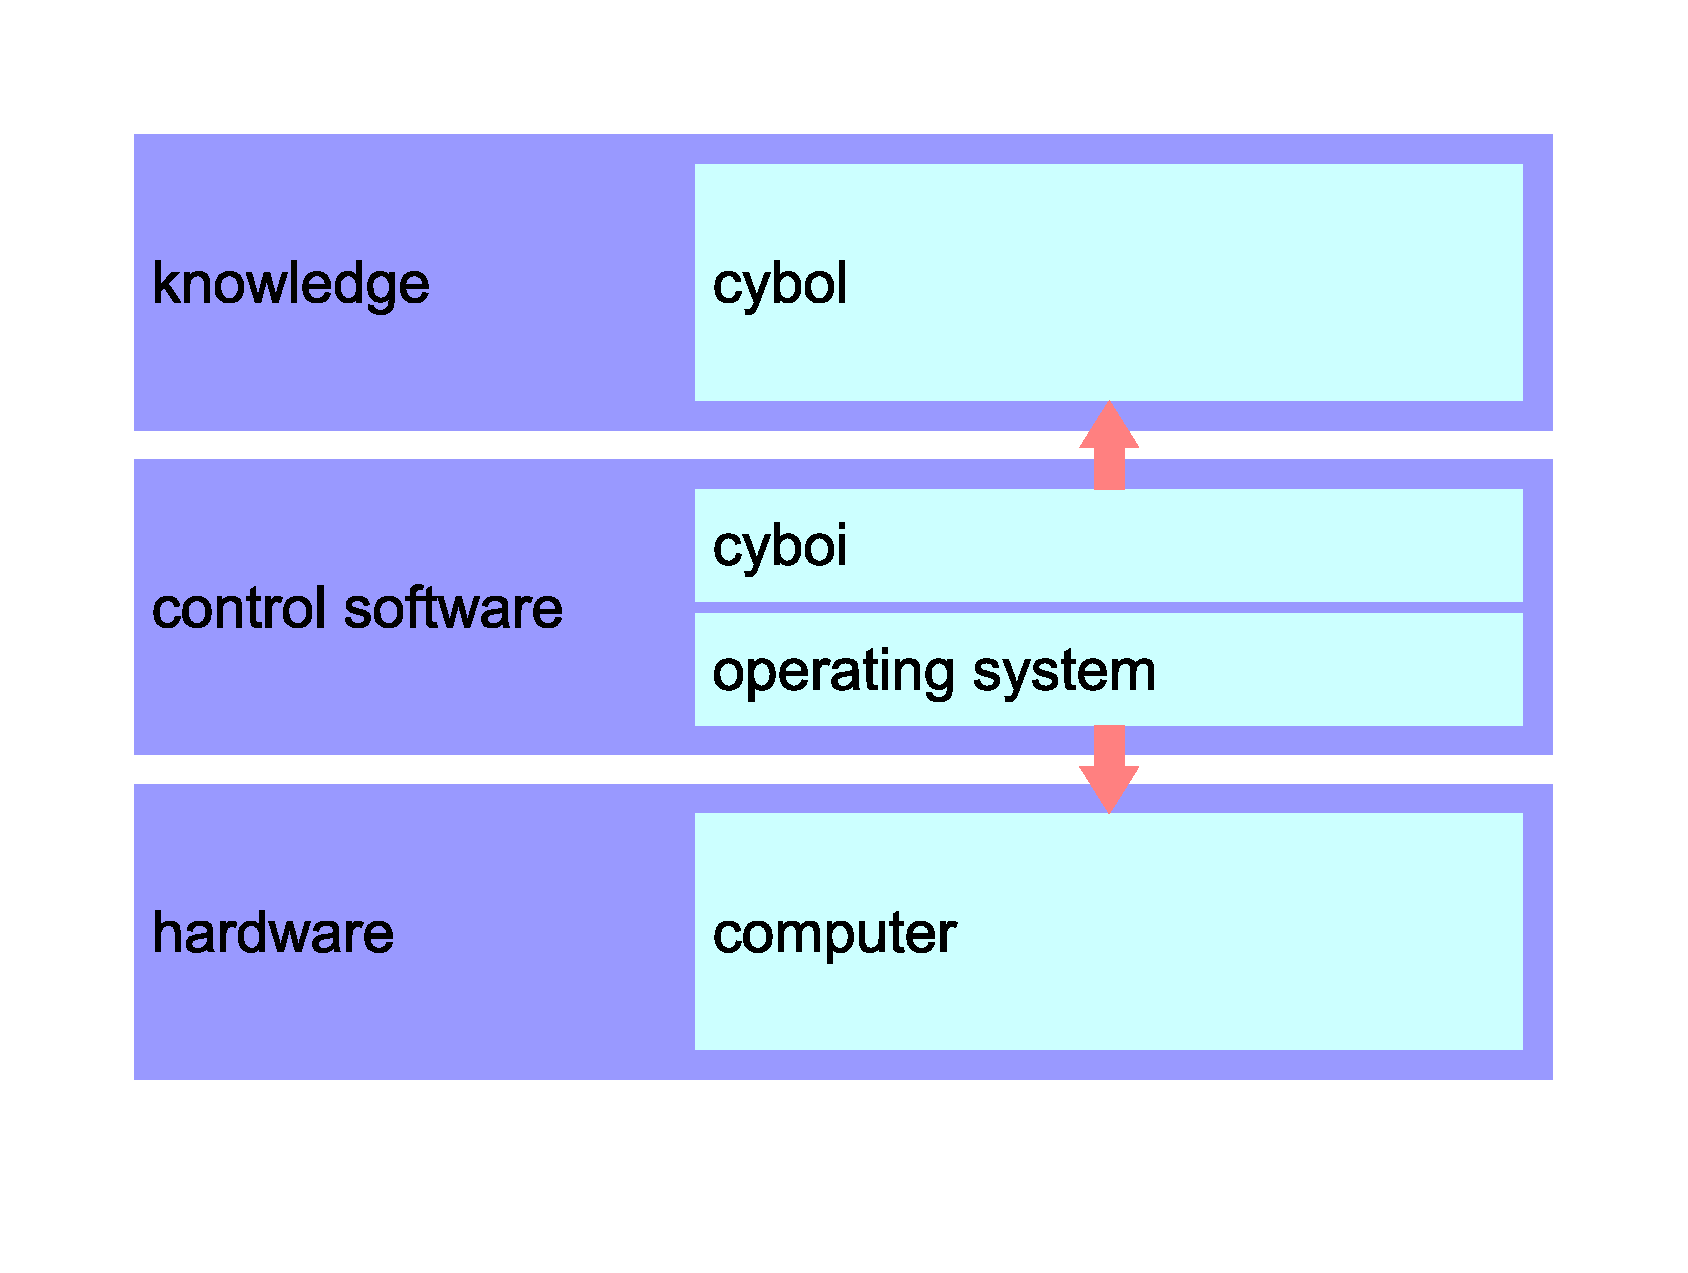
\includegraphics[scale=0.2]{vector/connection.eps}
        \caption{Knowledge -- Hardware Link}
        \label{connection_figure}
    \end{center}
\end{figure}

\begin{table}[ht]
    \begin{center}
        \begin{footnotesize}
        \begin{tabular}{| p{18mm} | p{18mm} | p{18mm} |}
            \hline
            \textbf{Criterion} & \textbf{Java World} & \textbf{CYBOP World}\\
            \hline
            Theory & OOP in Java & CYBOP\\
            \hline
            Language & Java & CYBOL\\
            \hline
            Interpreter & Java VM & CYBOI\\
            \hline
        \end{tabular}
        \end{footnotesize}
        \caption{Java-/ CYBOP World Analogies}
        \label{analogies_table}
    \end{center}
\end{table}

There are analogies to other systems run by language interpretation. Table
\ref{analogies_table} shows those between the \emph{Java-} and \emph{CYBOP}
world. Both are based on a programming theory, have a language and interpreter.
A theoretical model of a computer hardware- or -software system may be called
an \emph{Abstract Computer} or \emph{Abstract Machine} \cite{wikipedia}. If
being implemented as software simulation, or if containing an interpreter, it
is called a \emph{Virtual Machine} (VM). Kernighan and Pike write in their book
\emph{Practice of Programming} \cite{kernighan1999}:

\begin{quote}
� � Virtual machines are a wonderful, old idea, that latterly, through Java and
    the \emph{Java Virtual Machine} (JVM), came into fashion again. They are a
    simple possibility to gain portable and efficient program code, which can
    be written in a higher programming language.
\end{quote}

In that sense, CYBOI is certainly a VM. It provides low-level, platform-dependent
system functionality, close to the OS, together with a unified knowledge schema
(section \ref{knowledge_schema_heading}) which allows CYBOL applications to be
truly portable, well extensible and easier to program, because developers need
to concentrate on domain knowledge only. Since CYBOI interprets CYBOL sources
\emph{live} at system runtime, without the need for previous compilation (as in
Java), changes to CYBOL sources get into effect right away, without restarting
the system.

%
% $RCSfile$
%
% Copyright (c) 2005-2006. Christian Heller. All rights reserved.
%
% Permission is granted to copy, distribute and/or modify this document
% under the terms of the GNU Free Documentation License, Version 1.1 or
% any later version published by the Free Software Foundation; with no
% Invariant Sections, with no Front-Cover Texts and with no Back-Cover
% Texts. A copy of the license is included in the section entitled
% "GNU Free Documentation License".
%
% http://www.cybop.net
% - Cybernetics Oriented Programming -
%
% http://www.resmedicinae.org
% - Information in Medicine -
%
% Version: $Revision$ $Date$ $Author$
% Authors: Christian Heller <christian.heller@tuxtax.de>
%

\subsubsection{Architecture}
\label{architecture_heading}

To what concerns its inner architecture, there are two basic structures
underlying CYBOI:

\begin{enumerate}
    \item \emph{Knowledge Container:} An array-based structure usable for
        storing static knowledge in form of primitive- and compound models, and
        capable of representing a map, collection, list and tree
    \item \emph{Signal Checker:} A loop-based structure usable for dynamically
        reading signals from a queue, and capable of processing them after
        their priority, in a special handler
\end{enumerate}

\begin{figure}[ht]
    \begin{center}
        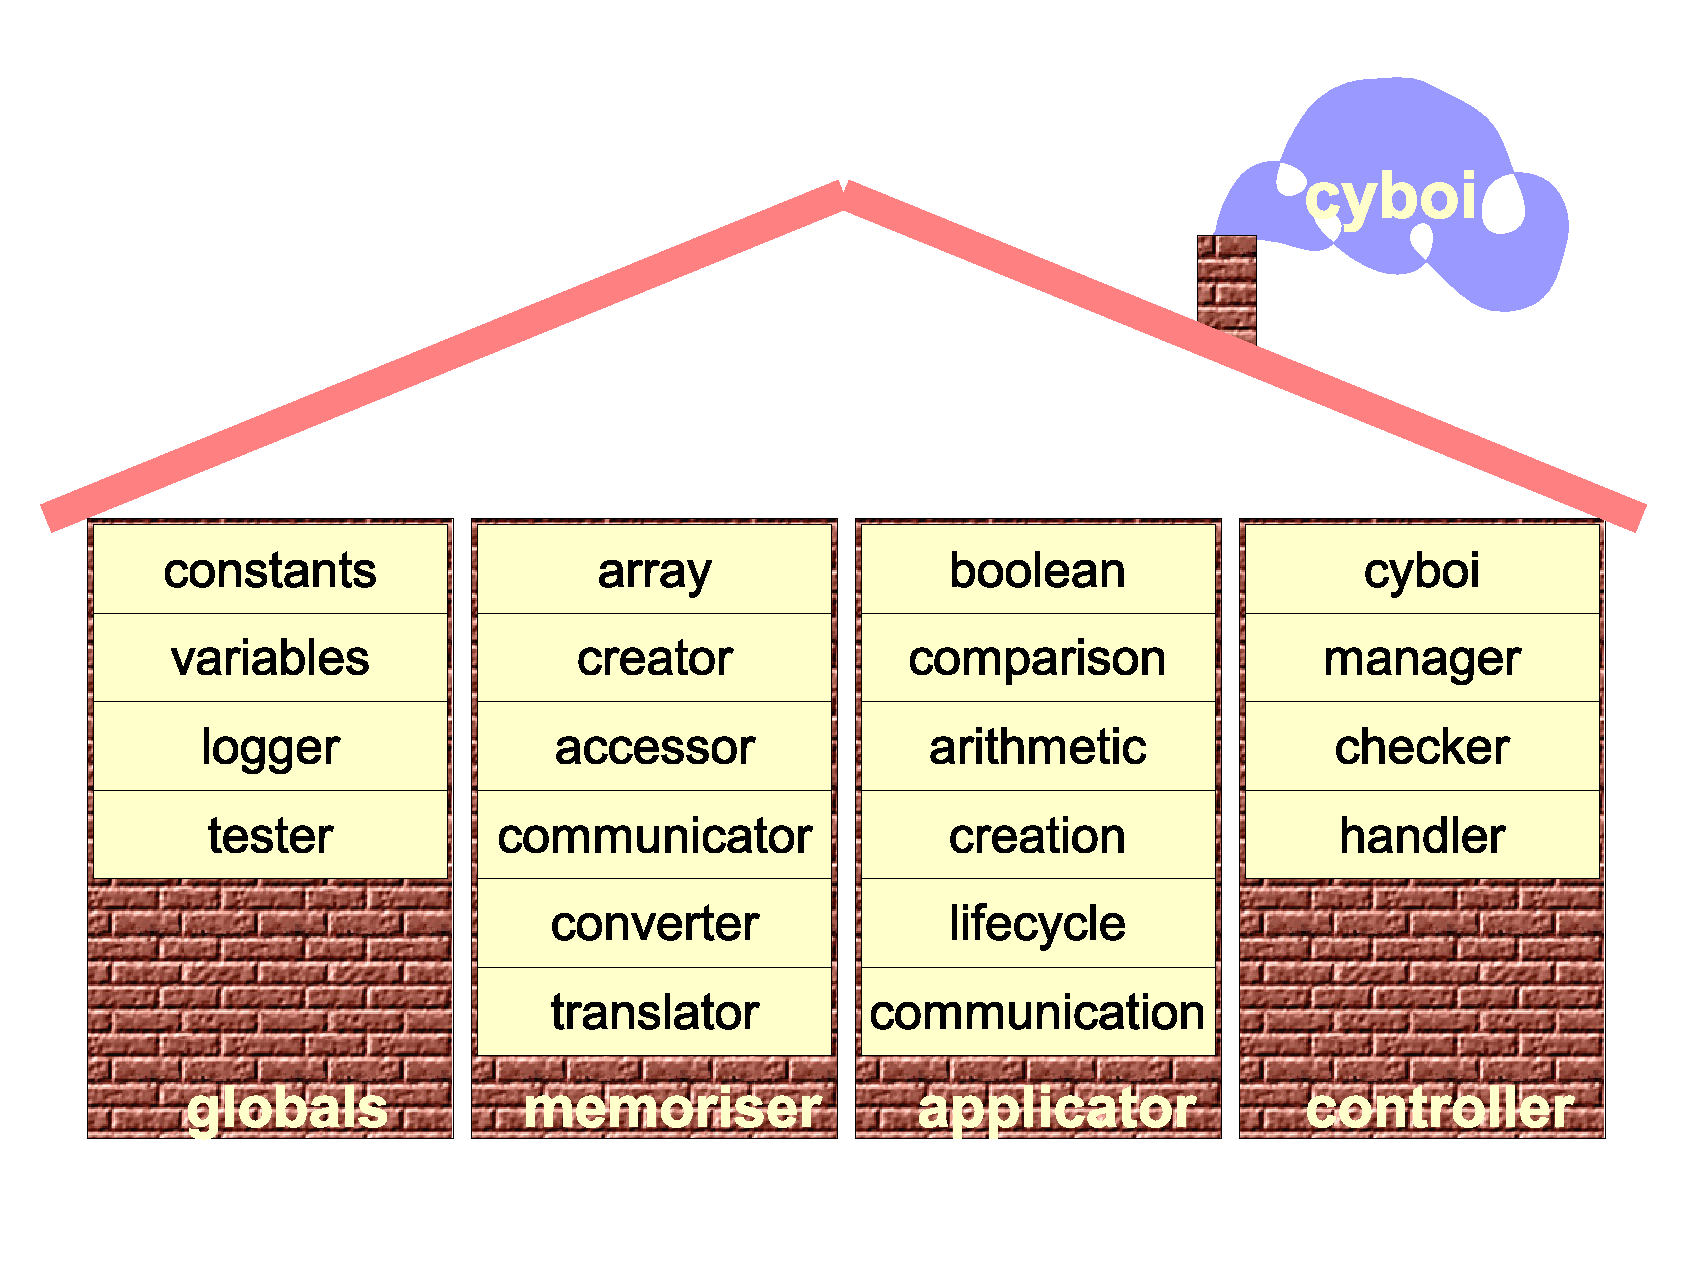
\includegraphics[scale=0.2]{vector/architecture.eps}
        \caption{CYBOI Architecture}
        \label{architecture_figure}
    \end{center}
\end{figure}

All modules, into which CYBOI is subdivided, are built around these two core
structures. Not unlike John von Neumann's model of a computing machine
\cite{selflinux}, which distinguishes \emph{Memory}, \emph{Control Unit},
\emph{Algorithmic Logic Unit} (ALU) and \emph{Input/ Output} (i/o), CYBOI's
modules are grouped into four architectural parts, as illustrated in figure
\ref{architecture_figure}. These have the following functionality:

\begin{itemize}
    \item \emph{Memoriser:} data creation, -destruction and -access (after
        Neumann, it contains not only data, but also the operations that are
        applied to them)
    \item \emph{Controller:} lifecycle management, signal handling, i/o filters
    \item \emph{Applicator:} operation application (comparison, logic,
        arithmetic and more)
    \item \emph{Globals:} basic constants and variables, as well as a logger
\end{itemize}

The i/o data handling is not separated out here (as opposed to von Neumann's
model); it is managed by the controller modules. The i/o data themselves,
representing states, are stored in memory.

%
% $RCSfile$
%
% Copyright (c) 2005-2006. Christian Heller. All rights reserved.
%
% Permission is granted to copy, distribute and/or modify this document
% under the terms of the GNU Free Documentation License, Version 1.1 or
% any later version published by the Free Software Foundation; with no
% Invariant Sections, with no Front-Cover Texts and with no Back-Cover
% Texts. A copy of the license is included in the section entitled
% "GNU Free Documentation License".
%
% http://www.cybop.net
% - Cybernetics Oriented Programming -
%
% http://www.resmedicinae.org
% - Information in Medicine -
%
% Version: $Revision$ $Date$ $Author$
% Authors: Christian Heller <christian.heller@tuxtax.de>
%

\subsubsection{Functionality}
\label{functionality_heading}

Figure \ref{cyboi_figure} shows three main parts of CYBOI. (The \emph{Globals}
package is neglectable for the following explanations, since it contains static
constants and variables that are \emph{omnipresent}.) The \emph{Controller}
manages system startup, shutdown and the handling of signals during its
runtime; the system uses just one central signal checking loop. The
\emph{Memoriser} provides memory structures (to store knowledge) and procedures
to access these. Logic knowledge is processed in the \emph{Applicator}.

\begin{figure}[ht]
    \begin{center}
        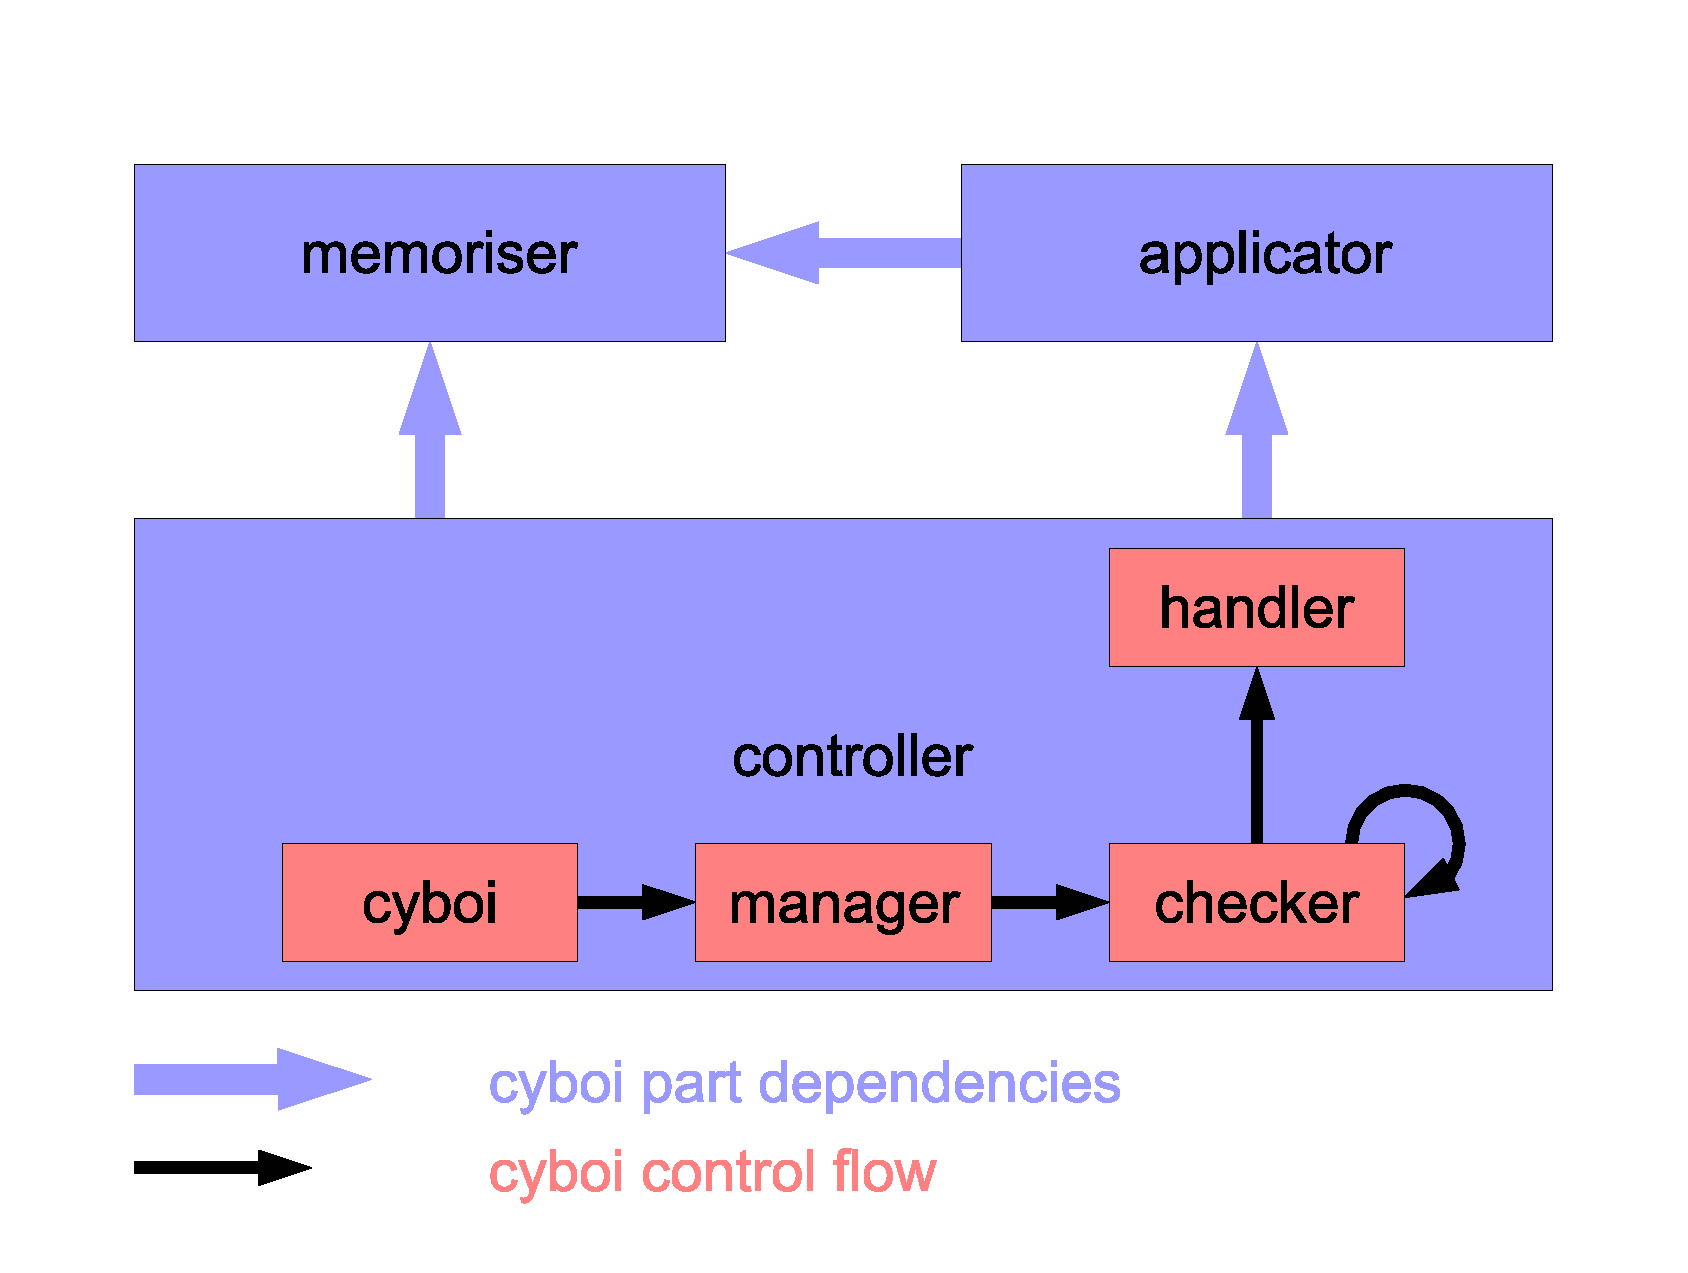
\includegraphics[scale=0.2]{vector/dependencies.eps}
        \caption{Dependencies and Control Flow}
        \label{cyboi_figure}
    \end{center}
\end{figure}


%
% $RCSfile: res_medicinae.tex,v $
%
% Copyright (C) 2002-2008. Christian Heller.
%
% Permission is granted to copy, distribute and/or modify this document
% under the terms of the GNU Free Documentation License, Version 1.1 or
% any later version published by the Free Software Foundation; with no
% Invariant Sections, with no Front-Cover Texts and with no Back-Cover
% Texts. A copy of the license is included in the section entitled
% "GNU Free Documentation License".
%
% http://www.cybop.net
% - Cybernetics Oriented Programming -
%
% http://www.resmedicinae.org
% - Information in Medicine -
%
% Version: $Revision: 1.1 $ $Date: 2008-08-19 20:41:08 $ $Author: christian $
% Authors: Christian Heller <christian.heller@tuxtax.de>
%

\chapter{Res Medicinae}
\label{res_medicinae_heading}
\index{Res Medicinae Application Prototype}

\begin{flushright}
    \textsl{
        No Road can ever be too long,\\
        side-by-side with a good Friend.
    }\\
    \textsc{Unknown Author}
\end{flushright}

The first two chapters (\ref{cybernetics_oriented_language_heading} and
\ref{cybernetics_oriented_interpreter_heading}) of part \ref{proof_heading} of
this work defined the CYBOL language and its corresponding interpreter CYBOI.
Since a theory is worth more if it can be proven in practice, this chapter will
describe an effort trying to apply both to create an application system named
\emph{Res Medicinae} \cite{resmedicinae} (Latin for \emph{Matter of Medicine}).

%
% $RCSfile: project.tex,v $
%
% Copyright (C) 2002-2008. Christian Heller.
%
% Permission is granted to copy, distribute and/or modify this document
% under the terms of the GNU Free Documentation License, Version 1.1 or
% any later version published by the Free Software Foundation; with no
% Invariant Sections, with no Front-Cover Texts and with no Back-Cover
% Texts. A copy of the license is included in the section entitled
% "GNU Free Documentation License".
%
% http://www.cybop.net
% - Cybernetics Oriented Programming -
%
% http://www.resmedicinae.org
% - Information in Medicine -
%
% Version: $Revision: 1.1 $ $Date: 2008-08-19 20:41:08 $ $Author: christian $
% Authors: Christian Heller <christian.heller@tuxtax.de>
%

\section{Project}
\label{project_heading}
\index{Res Medicinae Project}
\index{Hospital Information System}
\index{HIS}
\index{Practice Management System}
\index{PMS}
\index{Electronic Health Record}
\index{EHR}

The -- somewhat idealistic -- aim was initially to create the prototype of a
\emph{Hospital Information System} (HIS). Due to the clearly too high-set aims,
this was later revised so that the focus of the prototype became a standard
\emph{Practice Management System} (PMS) with an \emph{Electronic Health Record}
(EHR) as its core. Several technology changes during the progress of this work
and the lack in time required to also revise this aim, so that now the final
prototype consists of just the (rudimentary) address management module of the
planned EHR application. It is written in CYBOL and executable by CYBOI.

The following sections describe the project background of \emph{Res Medicinae}.

%
% $RCSfile: free_and_open_source_software.tex,v $
%
% Copyright (C) 2002-2008. Christian Heller.
%
% Permission is granted to copy, distribute and/or modify this document
% under the terms of the GNU Free Documentation License, Version 1.1 or
% any later version published by the Free Software Foundation; with no
% Invariant Sections, with no Front-Cover Texts and with no Back-Cover
% Texts. A copy of the license is included in the section entitled
% "GNU Free Documentation License".
%
% http://www.cybop.net
% - Cybernetics Oriented Programming -
%
% http://www.resmedicinae.org
% - Information in Medicine -
%
% Version: $Revision: 1.1 $ $Date: 2008-08-19 20:41:06 $ $Author: christian $
% Authors: Christian Heller <christian.heller@tuxtax.de>
%

\subsection{Free and Open Source Software}
\label{free_and_open_source_software_heading}
\index{Free and Open Source Software}
\index{FOSS}
\index{Free/ Libre Open Source Software}
\index{FLOSS}
\index{General Public License}
\index{GPL}
\index{Free Documentation License}
\index{FDL}
\index{Open Source Software}
\index{OSS}

Just like CYBOP (including CYBOL and CYBOI) \cite{cybop}, \emph{Res Medicinae}
\cite{resmedicinae} is developed within a \emph{Free/ Libre Open Source Software}
(FLOSS) project. Its source code, resources and documentation are placed under
GNU's \emph{General Public License} (GPL) (section
\ref{gnu_general_public_license_heading}) and \emph{Free Documentation License}
(FDL) (section \ref{gnu_free_documentation_license_heading}), respectively.
That means they can be freely redistributed and modified under the terms of
these licences. Although distributed in the hope that they will be useful, the
program and its resources come \emph{without any warranty}, without even the
implied warranty of \emph{merchantability or fitness for a particular purpose}.
See \cite{gnulicences} for details.

More information on \emph{Open Source Software} (OSS) in general can be found
at \cite{opensource}. There are plenty of resources for further background
reading, a German one being the \emph{Open Source Jahrbuch 2004}
\cite{opensourcejahrbuch2004}. To what concerns FLOSS in the medical arena,
many other projects exist. Comprehensive lists of these can be found at
\cite{euspirit, linuxmednews, medhowto}.

%
% $RCSfile: portals_and_services.tex,v $
%
% Copyright (C) 2002-2008. Christian Heller.
%
% Permission is granted to copy, distribute and/or modify this document
% under the terms of the GNU Free Documentation License, Version 1.1 or
% any later version published by the Free Software Foundation; with no
% Invariant Sections, with no Front-Cover Texts and with no Back-Cover
% Texts. A copy of the license is included in the section entitled
% "GNU Free Documentation License".
%
% http://www.cybop.net
% - Cybernetics Oriented Programming -
%
% http://www.resmedicinae.org
% - Information in Medicine -
%
% Version: $Revision: 1.1 $ $Date: 2008-08-19 20:41:08 $ $Author: christian $
% Authors: Christian Heller <christian.heller@tuxtax.de>
%

\subsection{Portals and Services}
\label{portals_and_services_heading}
\index{Open Source Development Portals and Services}
\index{Sourceforge Development Portal}
\index{Freshmeat Development Portal}
\index{BerliOS Development Portal}
\index{Savannah Development Portal}
\index{Free Software Foundation}
\index{FSF}

As OSS became popular over the years, the number of its supporters rose. It is
not long time that \emph{Sourceforge} \cite{sourceforge}, the first
\emph{Development Portal} for FLOSS, was opened. Shortly after, others like
\emph{Freshmeat} \cite{freshmeat} followed and meanwhile, there are also
national initiatives like \emph{BerliOS} \cite{berlios} in Germany. Also the
\emph{Free Software Foundation} (FSF) offers an own portal called
\emph{Savannah} \cite{savannah}, hosting exclusively \emph{free} \cite{gnu}
software projects. Figure \ref{portals_figure} shows the four portals by their
name, logo and \emph{Uniform Resource Locator} (URL).

\begin{figure}[ht]
    \begin{center}
        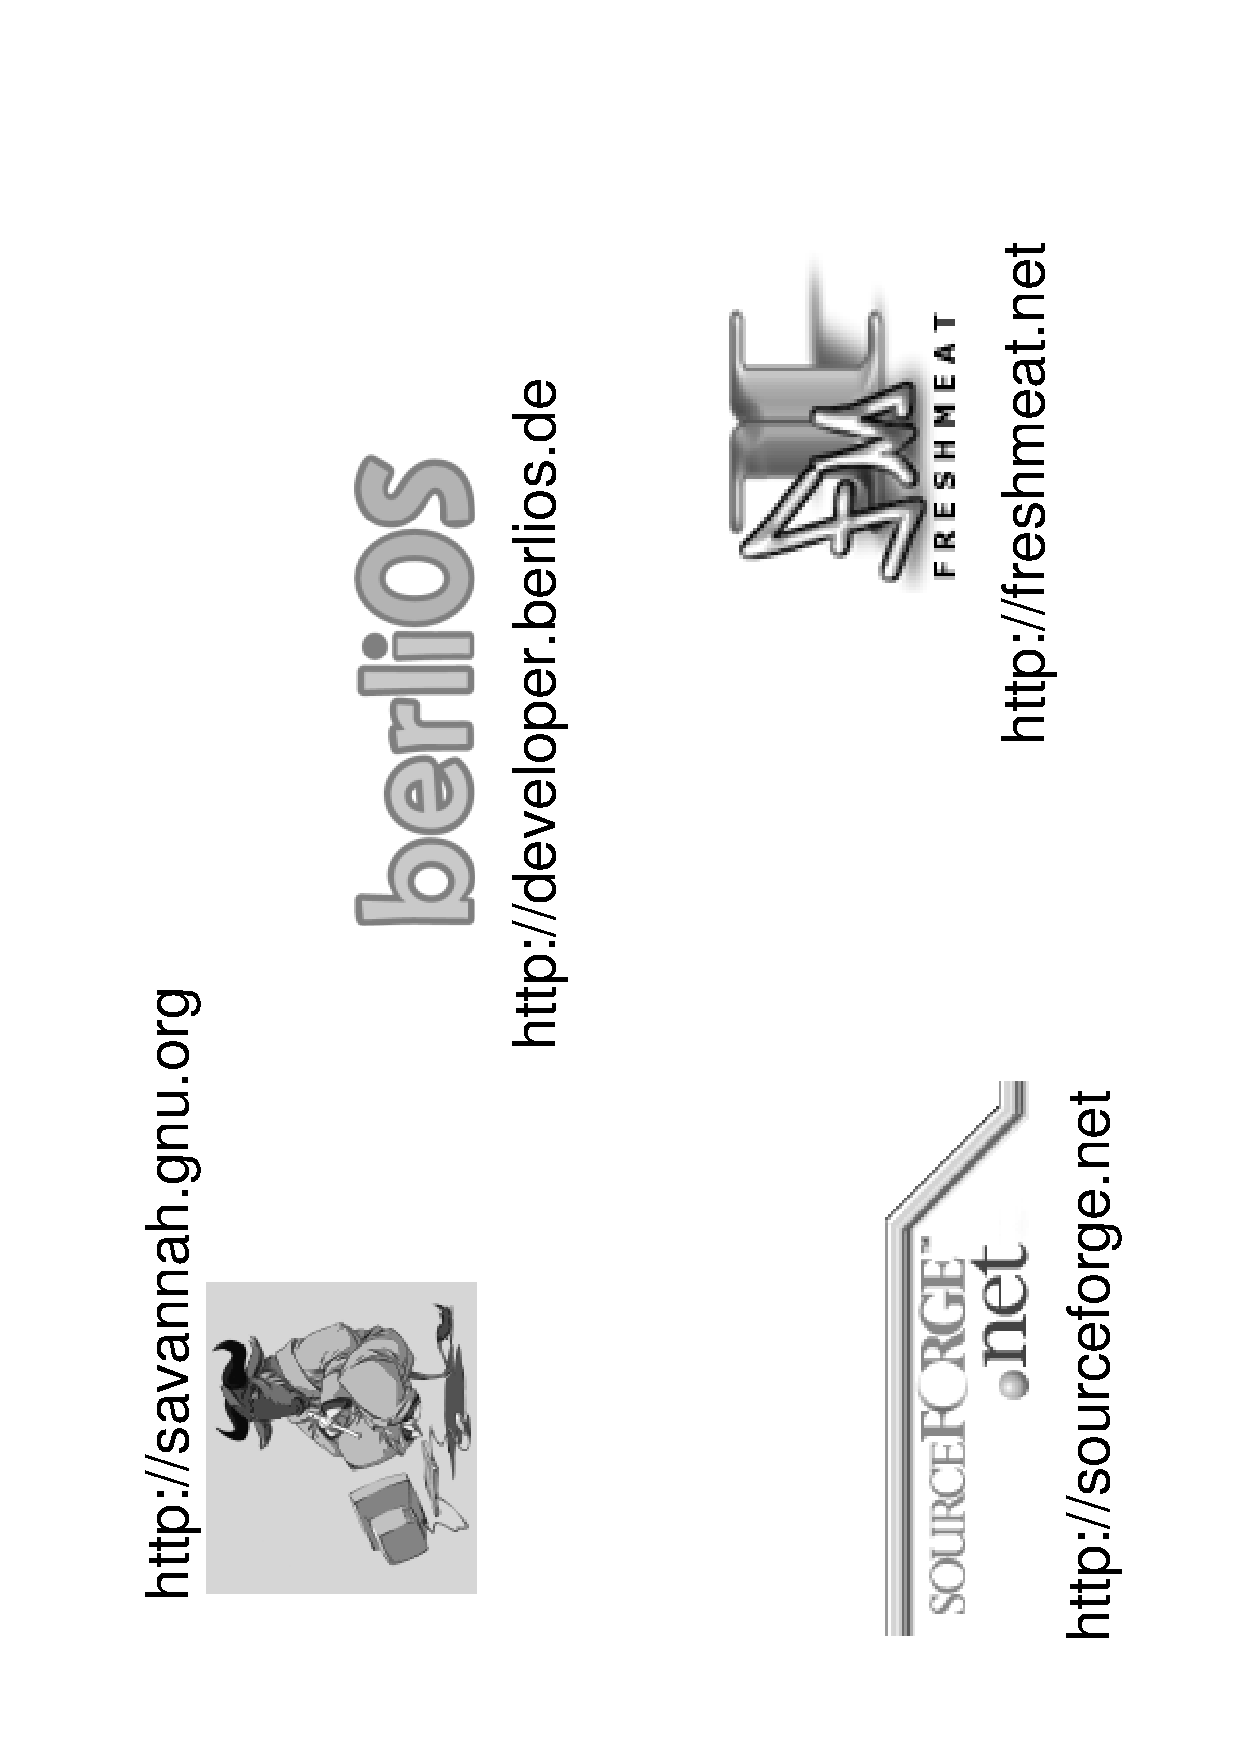
\includegraphics[scale=0.3,angle=-90]{graphic/portals.pdf}
        \caption{FLOSS Development Portals}
        \label{portals_figure}
    \end{center}
\end{figure}

As \emph{BerliOS} states in its slogan, it is the aim of development portals of
that kind to \textit{foster open source development}. In \emph{Savannah's}
words, they are \textit{central points for the development, distribution and
maintenance of FLOSS}. Although very often supported by well-known sponsors,
most portals are and want to stay independent. Using them, OSS projects and their
developers are offered several free services (figure \ref{services_figure}).
Since not all of these are always useful, projects can configure their portal
sites as needed.

\begin{figure}[ht]
    \begin{center}
        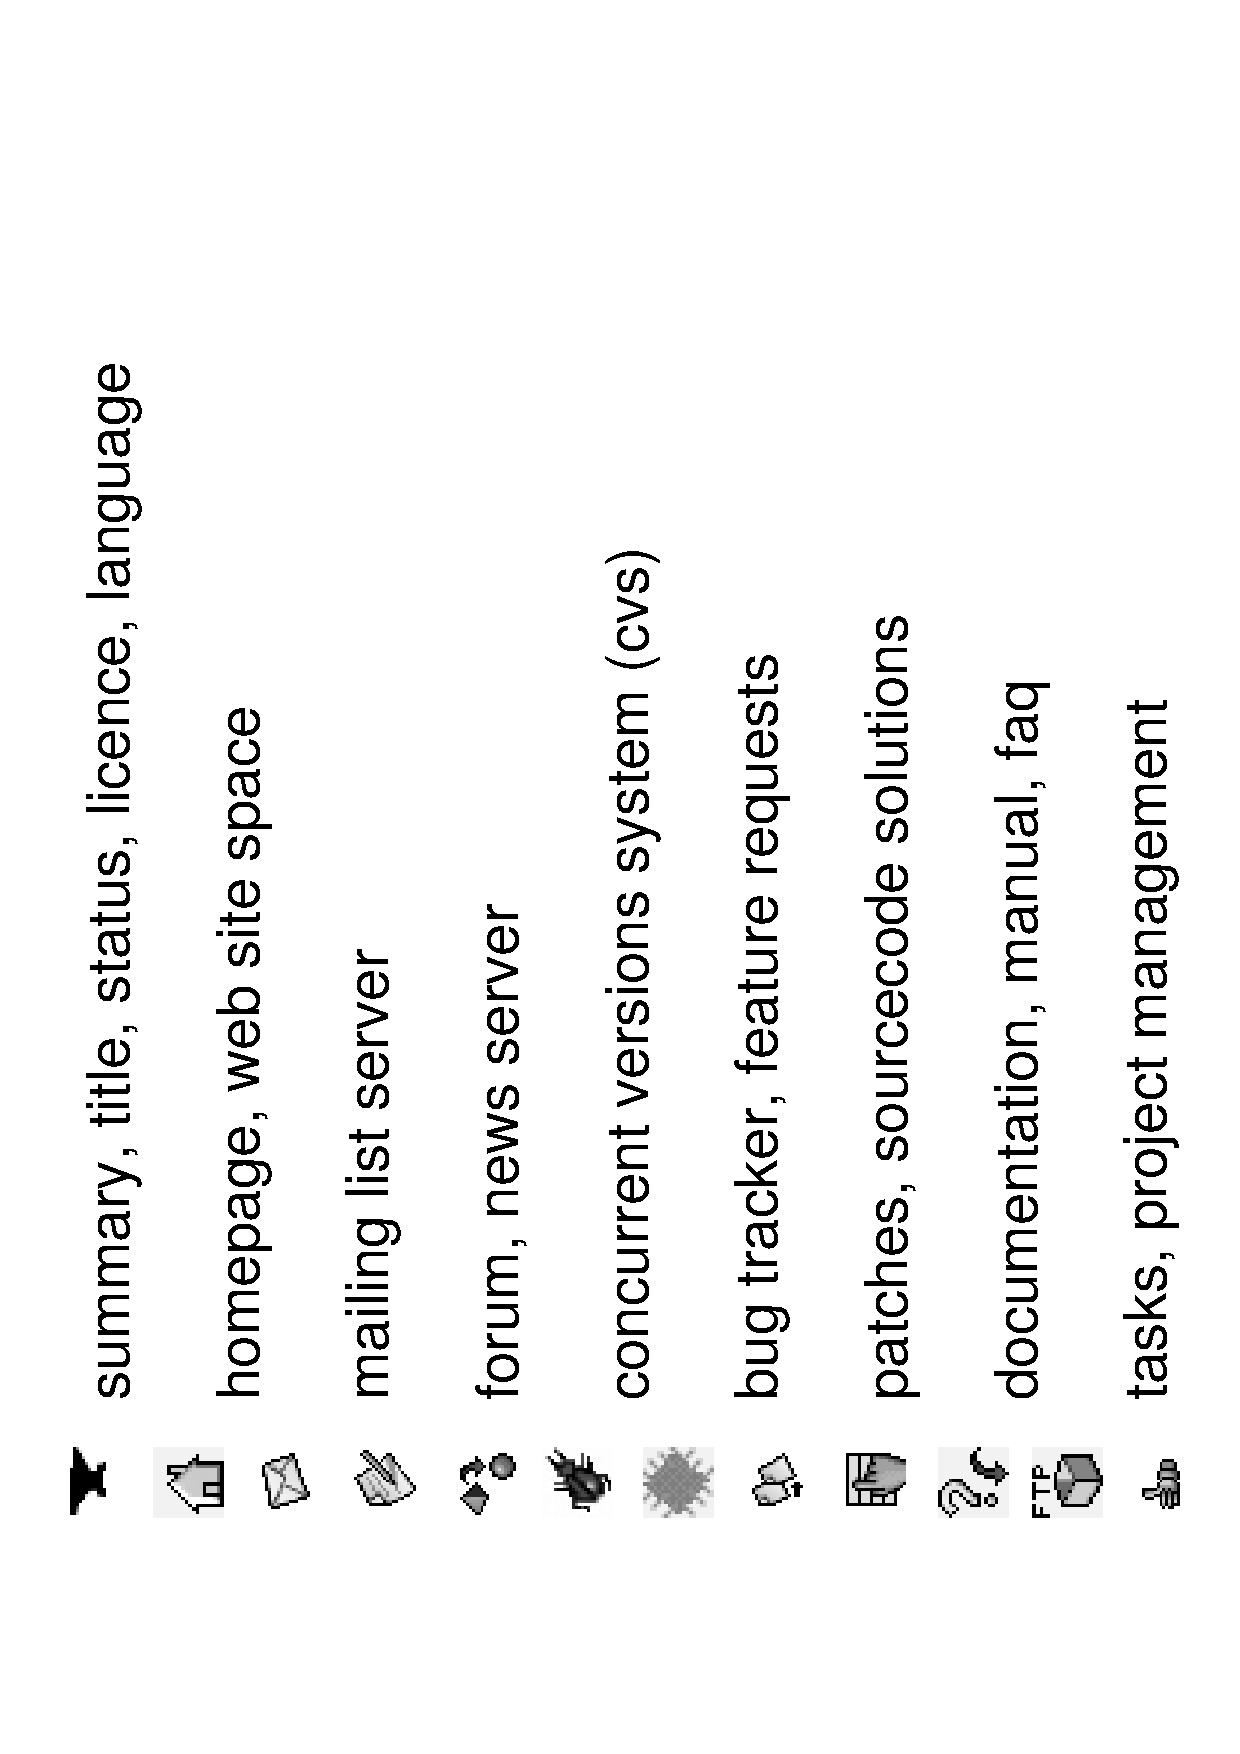
\includegraphics[scale=0.3,angle=-90]{graphic/services.pdf}
        \caption{Portal Services}
        \label{services_figure}
    \end{center}
\end{figure}

\emph{Res Medicinae} was one of the first OSS projects registered at
Sourceforge (number 4237 of now more than 100,000). CYBOP (CYBOL, CYBOI) is
hosted at BerliOS.

%
% $RCSfile: tools.tex,v $
%
% Copyright (C) 2002-2008. Christian Heller.
%
% Permission is granted to copy, distribute and/or modify this document
% under the terms of the GNU Free Documentation License, Version 1.1 or
% any later version published by the Free Software Foundation; with no
% Invariant Sections, with no Front-Cover Texts and with no Back-Cover
% Texts. A copy of the license is included in the section entitled
% "GNU Free Documentation License".
%
% http://www.cybop.net
% - Cybernetics Oriented Programming -
%
% http://www.resmedicinae.org
% - Information in Medicine -
%
% Version: $Revision: 1.1 $ $Date: 2008-08-19 20:41:09 $ $Author: christian $
% Authors: Christian Heller <christian.heller@tuxtax.de>
%

\subsection{Tools}
\label{tools_heading}
\index{Res Medicinae Development Tools}

Classical application development relies on tools like a \emph{UML Designer}, for
creating \emph{Unified Modeling Language} (UML) diagrams, a \emph{Text Editor},
\emph{Compiler} and \emph{Debugger}. Nowadays, these and other tools are
offered in one package, as \emph{Integrated Development Environment} (IDE).

Because the CYBOI interpreter is written in the system programming language
\emph{C}, its development requires a compiler. CYBOL applications, on the other
hand, do not have to be compiled. They base on interpreted XML code which can
be written in every text editor; nothing else is needed. An adapted editor was
proposed in section \ref{template_editor_heading}.

Res Medicinae development could certainly be speeded up by using graphical
diagrams in the style of the UML. But unfortunately, design tools that directly
support CYBOP do not exist yet. As section \ref{knowledge_designer_heading}
tried to show, some UML diagrams could be used with only minor adaptations for
CYBOL modelling. For the time being, standard XML editors have to suffice.

For running and testing CYBOL applications, of course, the CYBOI interpreter is
needed.

%
% $RCSfile: contributors.tex,v $
%
% Copyright (C) 2002-2008. Christian Heller.
%
% Permission is granted to copy, distribute and/or modify this document
% under the terms of the GNU Free Documentation License, Version 1.1 or
% any later version published by the Free Software Foundation; with no
% Invariant Sections, with no Front-Cover Texts and with no Back-Cover
% Texts. A copy of the license is included in the section entitled
% "GNU Free Documentation License".
%
% http://www.cybop.net
% - Cybernetics Oriented Programming -
%
% http://www.resmedicinae.org
% - Information in Medicine -
%
% Version: $Revision: 1.1 $ $Date: 2008-08-19 20:41:06 $ $Author: christian $
% Authors: Christian Heller <christian.heller@tuxtax.de>
%

\subsection{Contributors}
\label{contributors_heading}
\index{Res Medicinae Contributors}
\index{Open Source Health Care Alliance}
\index{OSHCA}

OSS projects are not only \emph{Hobby Activities} any longer. Many of them have
long overtaken their commercial competitors, in functionality, stability,
security and popularity. Due to the participation of sometimes hundreds of
enthusiasts, they mostly have much greater momentum.

In the case of \emph{Res Medicinae}, a number of \emph{Medical Doctors} (MD)
and \emph{Software Engineers} have contributed with their work or expressed
serious interest in collaboration. Many \emph{Informatics Students} were (and
are) involved and completed their diploma (master) works on a topic within the
project. Finally, there are the OSS projects that follow similar aims, like:

\begin{itemize}
    \item[-] \emph{GNUmed} \cite{gnumed}
    \item[-] \emph{Open Source Clinical Application Resource} (OSCAR) \cite{oscar}
    \item[-] \emph{Care2002} (Care2x) \cite{care2x}
    \item[-] \emph{Torch} \cite{torch}
    \item[-] \emph{Open Infrastructure for Outcomes} (OIO) \cite{oio}
    \item[-] \emph{Veterans Health Information Systems and Technology Architecture} (VistA) \cite{vista}
    \item[-] \emph{OpenEMed} \cite{openemed}
    \item[-] \emph{Tcl/Tk Family Practice} (tkFP) \cite{openehr}
    \item[-] \emph{Debian-Med} \cite{debianmed}, as meta project for packaging
\end{itemize}

All of them want to provide software solutions for medicine. Being friendly
concurrents, they use mailing lists such as \cite{openhealth} to exchange
latest insights, offer help to each other and work towards a better integration.
The technological decisions that have originally caused a division of forces
and a multitude of projects to exist, may in the end turn out to be fruitful,
with focus on the interoperability of systems. Additionally, organisations like
the \emph{Open Source Health Care Alliance} (OSHCA) \cite{oshca} bundle the
projects' forces and regularly organise conferences.


%
% $RCSfile: analysis.tex,v $
%
% Copyright (C) 2002-2008. Christian Heller.
%
% Permission is granted to copy, distribute and/or modify this document
% under the terms of the GNU Free Documentation License, Version 1.1 or
% any later version published by the Free Software Foundation; with no
% Invariant Sections, with no Front-Cover Texts and with no Back-Cover
% Texts. A copy of the license is included in the section entitled
% "GNU Free Documentation License".
%
% http://www.cybop.net
% - Cybernetics Oriented Programming -
%
% http://www.resmedicinae.org
% - Information in Medicine -
%
% Version: $Revision: 1.1 $ $Date: 2008-08-19 20:41:05 $ $Author: christian $
% Authors: Christian Heller <christian.heller@tuxtax.de>
%

\section{Analysis}
\label{analysis_heading}
\index{Res Medicinae Requirements Analysis}
\index{Software Engineering Process}
\index{SEP}
\index{Electronic Health Record}
\index{EHR}

Abiding by the standard \emph{Software Engineering Process} (SEP) (chapter
\ref{software_engineering_process_heading}), a \emph{Requirements Analysis}
stood as first activity for the development of \emph{Res Medicinae}. The
following sections will give a brief overview of some requirements and current
modelling trends, concerning the \emph{Electronic Health Record} (EHR). They do
\emph{not} try to replace more comprehensive works written on the subject.

%
% $RCSfile: requirements_document.tex,v $
%
% Copyright (C) 2002-2008. Christian Heller.
%
% Permission is granted to copy, distribute and/or modify this document
% under the terms of the GNU Free Documentation License, Version 1.1 or
% any later version published by the Free Software Foundation; with no
% Invariant Sections, with no Front-Cover Texts and with no Back-Cover
% Texts. A copy of the license is included in the section entitled
% "GNU Free Documentation License".
%
% http://www.cybop.net
% - Cybernetics Oriented Programming -
%
% http://www.resmedicinae.org
% - Information in Medicine -
%
% Version: $Revision: 1.1 $ $Date: 2008-08-19 20:41:08 $ $Author: christian $
% Authors: Christian Heller <christian.heller@tuxtax.de>
%

\subsection{Requirements Document}
\label{requirements_document_heading}
\index{Res Medicinae Requirements Document}
\index{DocBook DTD}
\index{The Linux Documentation Project}
\index{TLDP}

With the help of German medical doctors, a \emph{Requirements Document}
\cite{resmedicinae2001} was created and is meanwhile being updated and extended
since about five years. It basically describes an EHR and the information it
should include.

Since the document itself is just a hierarchical model consisting of parts, it
can well be represented in CYBOL. Unfortunately, a document processor that can
read and render CYBOL, in the style of \emph{LaTeX} \cite{latex}, has not been
written to date (although CYBOI might integrate this functionality one day). It
was therefore decided to write the requirements document in SGML/ XML, using
the \emph{DocBook} DTD \cite{docbook} and tools described in
\emph{The Linux Documentation Project} (TLDP) \cite{linuxdoc}.

%
% $RCSfile: ehr_and_co.tex,v $
%
% Copyright (C) 2002-2008. Christian Heller.
%
% Permission is granted to copy, distribute and/or modify this document
% under the terms of the GNU Free Documentation License, Version 1.1 or
% any later version published by the Free Software Foundation; with no
% Invariant Sections, with no Front-Cover Texts and with no Back-Cover
% Texts. A copy of the license is included in the section entitled
% "GNU Free Documentation License".
%
% http://www.cybop.net
% - Cybernetics Oriented Programming -
%
% http://www.resmedicinae.org
% - Information in Medicine -
%
% Version: $Revision: 1.1 $ $Date: 2008-08-19 20:41:06 $ $Author: christian $
% Authors: Christian Heller <christian.heller@tuxtax.de>
%

\subsection{EHR \& Co.}
\label{ehr_and_co_heading}
\index{Electronic Health Record}
\index{EHR}
\index{Personal Health Record}
\index{PHR}
\index{Virtual Health Record}
\index{VHR}
\index{Virtual Patient Record}
\index{VPR}
\index{Electronic Medical Record}
\index{EMR}
\index{Electronic Patient Record}
\index{EPR}
\index{Computer-based Patient Record}
\index{CPR}
\index{Computerised Patient Record}
\index{CPR}
\index{Computerised Medical Record}
\index{CMR}
\index{Automated Medical Record}
\index{AMR}
\index{Digital Medical Record}
\index{DMR}
\index{Patient Carried Record}
\index{PCR}
\index{Patient Medical Record}
\index{PMR}
\index{Integrated Care Record}
\index{ICR}
\index{Electronic Medical Infrastructure}
\index{EMI}
\index{Lifetime Data Repository}
\index{LDR}

Besides the now quite common term \emph{Electronic Health Record} (EHR), some
publications, experts or companies also talk of \cite{marietti, waegemann}:

\begin{itemize}
    \item[-] \emph{Personal Health Record} (PHR)
    \item[-] \emph{Virtual Health Record} (VHR)
    \item[-] \emph{Virtual Patient Record} (VPR)
    \item[-] \emph{Electronic Medical Record} (EMR)
    \item[-] \emph{Electronic Patient Record} (EPR)
    \item[-] \emph{Computer-based Patient Record} (CPR)
    \item[-] \emph{Computerised Patient Record} (CPR)
    \item[-] \emph{Computerised Medical Record} (CMR)
    \item[-] \emph{Automated Medical Record} (AMR)
    \item[-] \emph{Digital Medical Record} (DMR)
    \item[-] \emph{Patient Carried Record} (PCR)
    \item[-] \emph{Patient Medical Record} (PMR)
    \item[-] \emph{Integrated Care Record} (ICR)
    \item[-] \emph{Electronic Medical Infrastructure} (EMI)
    \item[-] \emph{Lifetime Data Repository} (LDR)
\end{itemize}

and state differences in their contents, access, maintainer, place of storage,
technology or other aspects. David Kibbe, for example, as cited by Jennifer
Bush \cite{bush}, says:

\begin{quote}
    There's recently been a subtle shift in terminology. EMR connotes a tool
    that's for doctors only and something that replaces the paper record with a
    database. EHR connotes more of a connectivity tool that not only includes
    the patient and may even be used by the patient, but also provides a set of
    tools to improve work-flow efficiency and quality of care in doctors' offices.

    \ldots\ An EHR should include a detailed clinical documentation function;
    prescription ordering and management capabilities; a secure messaging
    system; lab and test result reporting functions; evidence-based health
    guidelines; secure patient access to health records; a public health
    reporting- and tracking system; mapping to clinical- and standard code sets
    and the ability to interface with leading practice management software.
\end{quote}

In essence, however, most of the above-listed terms are considered synonymous,
since their definitions, if existent at all, differ just in nuances. Charlene
Marietti, who investigated in this subject, writes \cite{marietti}:

\begin{quote}
    Meanwhile, most practical people don't see a big difference between the CPR
    and the EMR and the many other terms that exist.
\end{quote}

Therefore, this work further on sticks to the term \emph{EHR} and wants it
understood as general description for either of the other terms mentioned
above.

%
% $RCSfile: episode_based.tex,v $
%
% Copyright (C) 2002-2008. Christian Heller.
%
% Permission is granted to copy, distribute and/or modify this document
% under the terms of the GNU Free Documentation License, Version 1.1 or
% any later version published by the Free Software Foundation; with no
% Invariant Sections, with no Front-Cover Texts and with no Back-Cover
% Texts. A copy of the license is included in the section entitled
% "GNU Free Documentation License".
%
% http://www.cybop.net
% - Cybernetics Oriented Programming -
%
% http://www.resmedicinae.org
% - Information in Medicine -
%
% Version: $Revision: 1.1 $ $Date: 2008-08-19 20:41:06 $ $Author: christian $
% Authors: Christian Heller <christian.heller@tuxtax.de>
%

\subsection{Episode Based}
\label{episode_based_heading}
\index{Episode Based EHR}
\index{Patient Centered Medical Record}
\index{Health Issue of an Episode Based EHR}
\index{Clinical Episode of an Episode Based EHR}
\index{Clinical Encounter of an Episode Based EHR}
\index{Clinical Item of an Episode Based EHR}
\index{Partial Contact of an Episode Based EHR}
\index{Problem Oriented Medical Record}
\index{POMR}

Historically, it took a long time until the concept of a modern EHR crystalised
out. An early form of a time-oriented medical record stems from Hippocrates
(5th century BC) who wanted to accurately reflect the course of a disease and
indicate its possible causes. In 1907, the \emph{Mayo Clinic} (formed by the
American surgeon William Mayo) adopted one separate file for each patient, to
be able to obtain a better overview of his complete disease history. This
innovation was the origin of the \emph{Patient Centered Medical Record} as
known today, as \cite{mihandbook} means.

The discussion on how to model an ideal EHR already lasts for decades and has
not finished. Recent proposals brought in some new perspectives and ideas. One
of them turns around the so-called \emph{Episode-based} EHR \cite{westerhof}.
In the centre of these considerations stands a structure that is described in a
more pragmatic way by Karsten Hilbert of GNUmed \cite{gnumed}. He sees a
complex EHR as hierarchical composition of the following items:

\begin{itemize}
    \item[-] Health Issue
    \item[-] Clinical Episode
    \item[-] Clinical Encounter
    \item[-] Clinical Item
\end{itemize}

The additional concept of a \emph{Partial Contact} as known from the Dutch
\emph{Episode Model} does not integrate into this hierarchy. But after Hilbert,
\emph{Partial Contacts} could be easily derived from existing EHR data by
aggregating all \emph{Clinical Items} that belong to the same
\emph{Clinical Encounter} and the same \emph{Clinical Episode}.

\emph{Clinical Items} are typically elements in the \emph{SOAP} format of
progress notes, as known from the \emph{Problem Oriented Medical Record} (POMR)
\cite{weed} that was introduced by Lawrence L. Weed in the 1960s. SOAP stands
for:

\begin{itemize}
    \item[-] \emph{Subjective:} Complaints as phrased by the patient
    \item[-] \emph{Objective:} Findings of physicians and nurses
    \item[-] \emph{Assessment:} Test results and conclusions, such as a diagnosis
    \item[-] \emph{Plan:} Medical plan, for example treatment or policy
\end{itemize}

%
% $RCSfile: evidence_based.tex,v $
%
% Copyright (C) 2002-2008. Christian Heller.
%
% Permission is granted to copy, distribute and/or modify this document
% under the terms of the GNU Free Documentation License, Version 1.1 or
% any later version published by the Free Software Foundation; with no
% Invariant Sections, with no Front-Cover Texts and with no Back-Cover
% Texts. A copy of the license is included in the section entitled
% "GNU Free Documentation License".
%
% http://www.cybop.net
% - Cybernetics Oriented Programming -
%
% http://www.resmedicinae.org
% - Information in Medicine -
%
% Version: $Revision: 1.1 $ $Date: 2008-08-19 20:41:06 $ $Author: christian $
% Authors: Christian Heller <christian.heller@tuxtax.de>
%

\subsection{Evidence Based}
\label{evidence_based_heading}
\index{Evidence Based EHR}
\index{Virtual Record (EHR)}

In an email to the \emph{Open Health Mailing List} \cite{openhealth}, David R.
raised a number of unsolved issues concerning the \emph{Evidence-based} EHR.
In a first thought, he exposes the existence of two distinct views on an EHR:
\emph{clinical} and \emph{evidential}. A medical record were not just a
collection of clinical information, but also a \emph{Legal Document} with
financial importance. It were to give evidence of the healthcare services
rendered by a particular provider for a particular organisation, and the reason
why, mostly, patients do not own the record. Finally, an EHR were the result of
the intersection of two major business processes: the \emph{Clinical Process}
and the \emph{Records Management Process}.

This observation leads to the second important question whether records should
be \emph{accessed} remotely, leaving them in place at each of the organisations
where the patient has been seen, or be \emph{incorporated} as extract or full
copy to each organisation's repository, as known from the paper-based world.
Since the first method, promoted as trans-organisational \emph{Virtual Record},
did not address an organisation's need for maintaining its evidential records,
it had, in the opinion of David R., failed to gain widespread or long-term
acceptance.

A third point turns around the authoring of an EHR. Record keeping were no
longer simply a \emph{personal} activity but rather an \emph{inter-personal}
action. David R. writes on:

\begin{quote}
    Historically, providers have viewed the medical records they have created
    as though they were a personal journal kept by the provider to facilitate
    his or her process of delivering care to an individual patient. It was
    viewed as an aid to memory and extended the provider's thought across time.
    \ldots\ In the setting of a highly mobile population of patients and
    providers, the record becomes a living document with multiple authors.
    Multiple individuals for multiple reasons consult it and \ldots\ it is in
    this record that a shared understanding of the (health) problems and
    recommended solutions for \ldots\ the individual occur.
\end{quote}

Because the EHR could be seen as a space for collaboration, applications
working with it had to support clinical process \emph{Workflow} requirements. A
new set of demands were also placed on health care providers, to document their
activities with patients in a way that is mutually \emph{intelligible} to those
who have a stake in the information contained in the record.

%
% $RCSfile: continuity_of_care.tex,v $
%
% Copyright (C) 2002-2008. Christian Heller.
%
% Permission is granted to copy, distribute and/or modify this document
% under the terms of the GNU Free Documentation License, Version 1.1 or
% any later version published by the Free Software Foundation; with no
% Invariant Sections, with no Front-Cover Texts and with no Back-Cover
% Texts. A copy of the license is included in the section entitled
% "GNU Free Documentation License".
%
% http://www.cybop.net
% - Cybernetics Oriented Programming -
%
% http://www.resmedicinae.org
% - Information in Medicine -
%
% Version: $Revision: 1.1 $ $Date: 2008-08-19 20:41:06 $ $Author: christian $
% Authors: Christian Heller <christian.heller@tuxtax.de>
%

\subsection{Continuity of Care}
\label{continuity_of_care_heading}
\index{Continuity of Care Record}
\index{CCR}
\index{Personal Health Project}
\index{PHP}

A main result of the opinion stated in the previous section was the realisation
that a major challenge for EHR design will be to overcome the difference
between an organisation's evidential record management process with emphasis on
\emph{legal/ financial aspects} and the record keeping as
\emph{medical/ health documentation}, that an individual would do.

This is exactly the issue that Philippe Ameline and his French colleagues
address in their \emph{Nautilus/ Odyssee} project \cite{nautilus}. It
distinguishes between three levels of data:

\begin{itemize}
    \item[-] \emph{Individual}: personal, various local
    \item[-] \emph{Group}: professional, 24 hour availability
    \item[-] \emph{Collective}: dedicated to continuity of care
\end{itemize}

The latter is called \emph{Personal Health Project} (PHP). Its health management
data can be shared between a \emph{Patient} and his \emph{Care Team}, with the
EHR \emph{passing by} institutions. Ameline writes in \cite{openehrtechnical}
that the management of these two referentials -- health professional and patient
-- meant that applications now had to handle differently the \emph{history data}
with a time duration (which may get changed by someone else) and the data of the
\emph{instantaneous picture} kind (what one noticed and reported at a given time).

A similar effort with U.S. American roots is called \emph{Continuity of Care Record}
(CCR) \cite{ccr}. Just like the PHP, it does not want to be a complete EHR, but
rather: \textit{organise and make transportable a set of basic patient
information consisting of the most relevant and timely facts about a patient's
condition.} Through specified XML code, the CCR becomes interoperable.

%
% $RCSfile: core_model.tex,v $
%
% Copyright (C) 2002-2008. Christian Heller.
%
% Permission is granted to copy, distribute and/or modify this document
% under the terms of the GNU Free Documentation License, Version 1.1 or
% any later version published by the Free Software Foundation; with no
% Invariant Sections, with no Front-Cover Texts and with no Back-Cover
% Texts. A copy of the license is included in the section entitled
% "GNU Free Documentation License".
%
% http://www.cybop.net
% - Cybernetics Oriented Programming -
%
% http://www.resmedicinae.org
% - Information in Medicine -
%
% Version: $Revision: 1.1 $ $Date: 2008-08-19 20:41:06 $ $Author: christian $
% Authors: Christian Heller <christian.heller@tuxtax.de>
%

\subsection{Core Model}
\label{core_model_heading}
\index{Res Medicinae Core Model}
\index{Electronic Health Record as Core Model}

Many kinds of application modules are needed in a healthcare-specific
\emph{Information Technology} (IT) environment. The tasks they fulfill,
together with a proposed name within the \emph{Res Medicinae} project, are
listed following:

\begin{itemize}
    \item[-] \emph{Revue:} Portal for module starting
    \item[-] \emph{Residenz:} Administrative data management
    \item[-] \emph{Record:} Clinical documentation
    \item[-] \emph{Rezept:} Prescription ordering and management
    \item[-] \emph{Reform:} Form printing
    \item[-] \emph{Report:} Public health reporting and tracking
    \item[-] \emph{Reagenz:} Laboratory- and test result retrieval
    \item[-] \emph{Rendezvous:} Scheduling
    \item[-] \emph{Roentgen:} Clinical imaging
    \item[-] \emph{Rechnung:} Billing
    \item[-] \emph{Richtig:} Statistics
    \item[-] \emph{Register:} Pharmaceutical reference
    \item[-] \emph{Ratlos:} Lexicon-, terminology- and code set query
\end{itemize}

\begin{figure}[ht]
    \begin{center}
        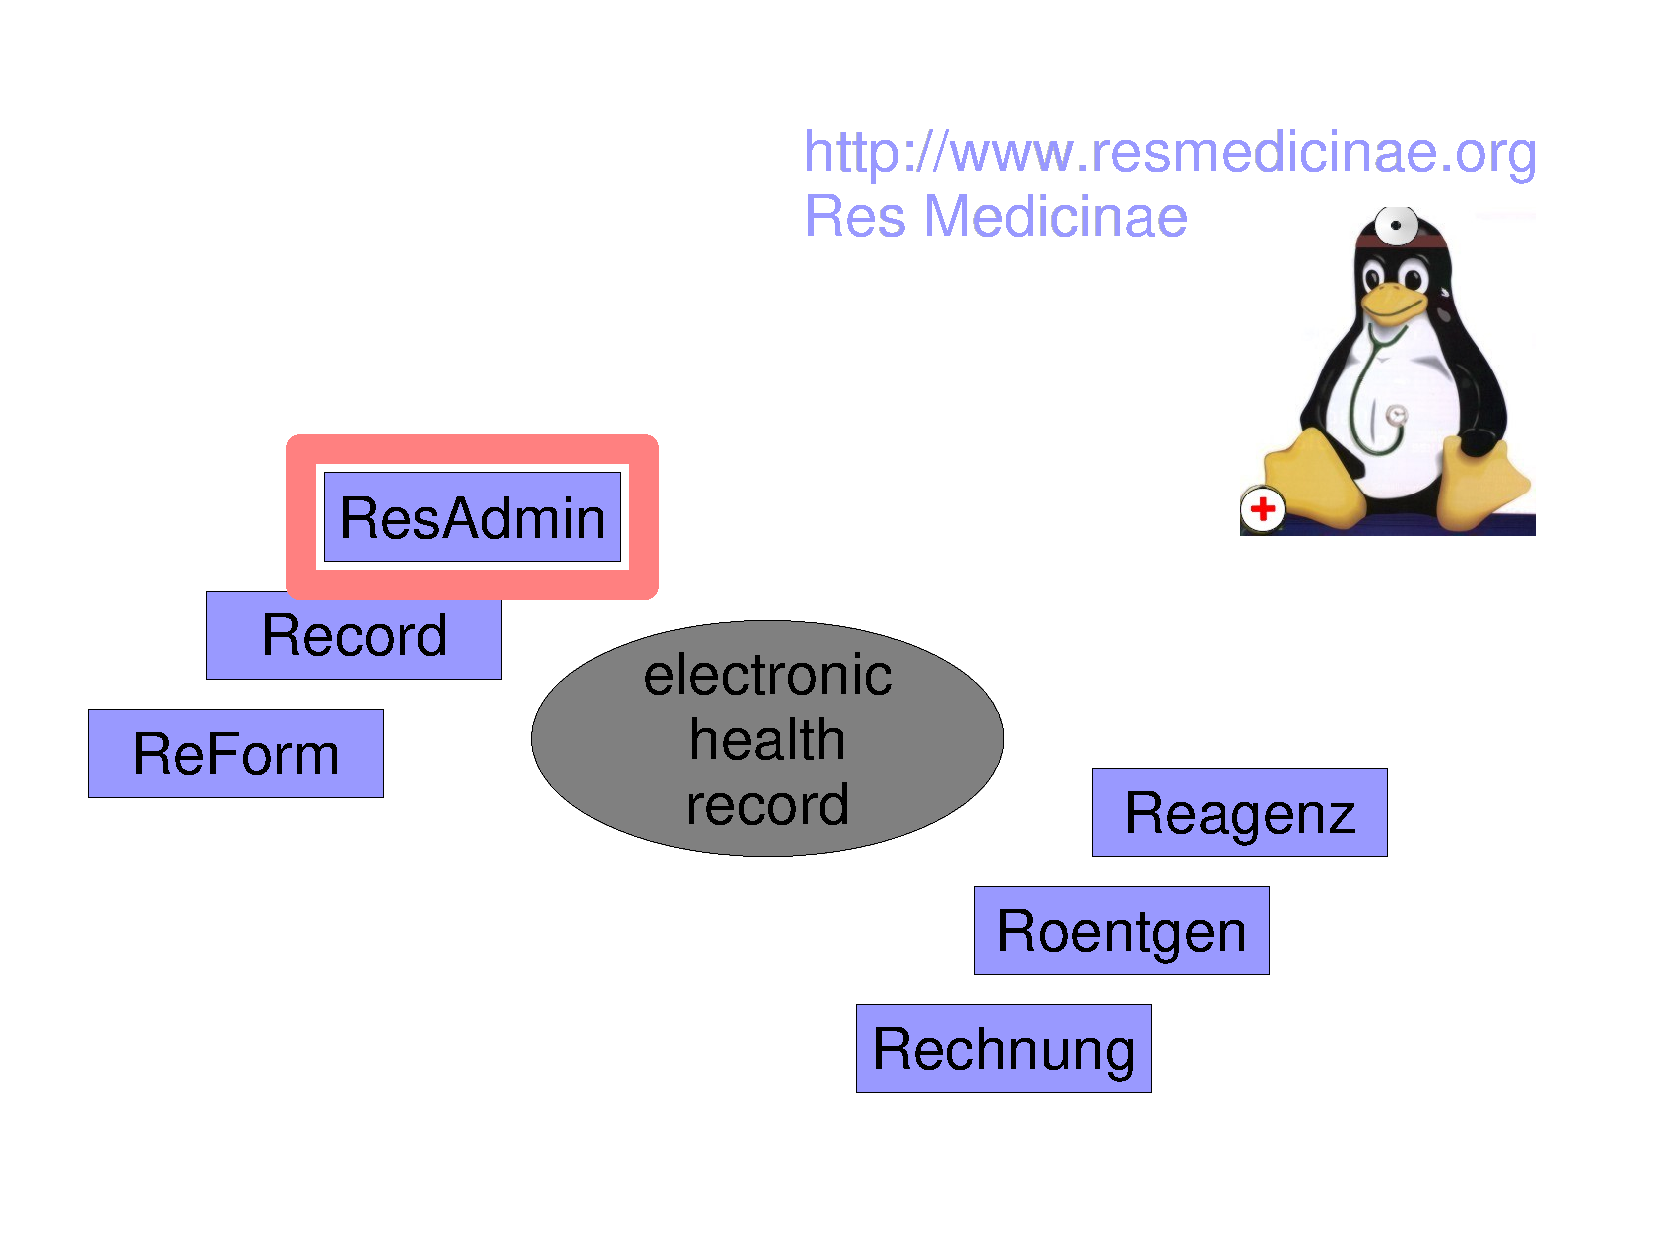
\includegraphics[scale=0.3,angle=-90]{graphic/core.pdf}
        \caption{Applications Grouped around an Electronic Health Record Core}
        \label{core_figure}
    \end{center}
\end{figure}

Figure \ref{core_figure} shows some of these modules, together with an EHR as
their central data structure.


\newpage
%
% $RCSfile: standards.tex,v $
%
% Copyright (C) 2002-2008. Christian Heller.
%
% Permission is granted to copy, distribute and/or modify this document
% under the terms of the GNU Free Documentation License, Version 1.1 or
% any later version published by the Free Software Foundation; with no
% Invariant Sections, with no Front-Cover Texts and with no Back-Cover
% Texts. A copy of the license is included in the section entitled
% "GNU Free Documentation License".
%
% http://www.cybop.net
% - Cybernetics Oriented Programming -
%
% http://www.resmedicinae.org
% - Information in Medicine -
%
% Version: $Revision: 1.1 $ $Date: 2008-08-19 20:41:09 $ $Author: christian $
% Authors: Christian Heller <christian.heller@tuxtax.de>
%

\section{Standards}
\label{standards_heading}
\index{Medical Informatics Standards}

In a further thought, current standards of medical informatics had to be
considered for the development of \emph{Res Medicinae} application modules.
There exists a whole plethora of (partly \emph{de facto}) standards -- far too
many to discuss here. The following sections will give a brief overview of only
a few standards which are potentially important for EHR development.

%
% $RCSfile: overview.tex,v $
%
% Copyright (C) 2002-2008. Christian Heller.
%
% Permission is granted to copy, distribute and/or modify this document
% under the terms of the GNU Free Documentation License, Version 1.1 or
% any later version published by the Free Software Foundation; with no
% Invariant Sections, with no Front-Cover Texts and with no Back-Cover
% Texts. A copy of the license is included in the section entitled
% "GNU Free Documentation License".
%
% http://www.cybop.net
% - Cybernetics Oriented Programming -
%
% http://www.resmedicinae.org
% - Information in Medicine -
%
% Version: $Revision: 1.1 $ $Date: 2008-08-19 20:41:08 $ $Author: christian $
% Authors: Christian Heller <christian.heller@tuxtax.de>
%

\subsection{Overview}
\label{overview_heading}
\index{Medical Informatics Working Groups}
\index{Deutsches Institut fuer Normung}
\index{DIN}
\index{Comite Europeen de Normalisation}
\index{CEN}
\index{International Organization for Standardization}
\index{ISO}

Figure \ref{groups_figure} shows the medical informatics working groups of
important standardisation organisations, namely the:

\begin{itemize}
    \item[-] \emph{Deutsches Institut fuer Normung} (DIN)
    \item[-] \emph{Comite Europeen de Normalisation} (CEN)
    \item[-] \emph{International Organization for Standardization} (ISO)
\end{itemize}

\begin{figure}[ht]
    \begin{center}
        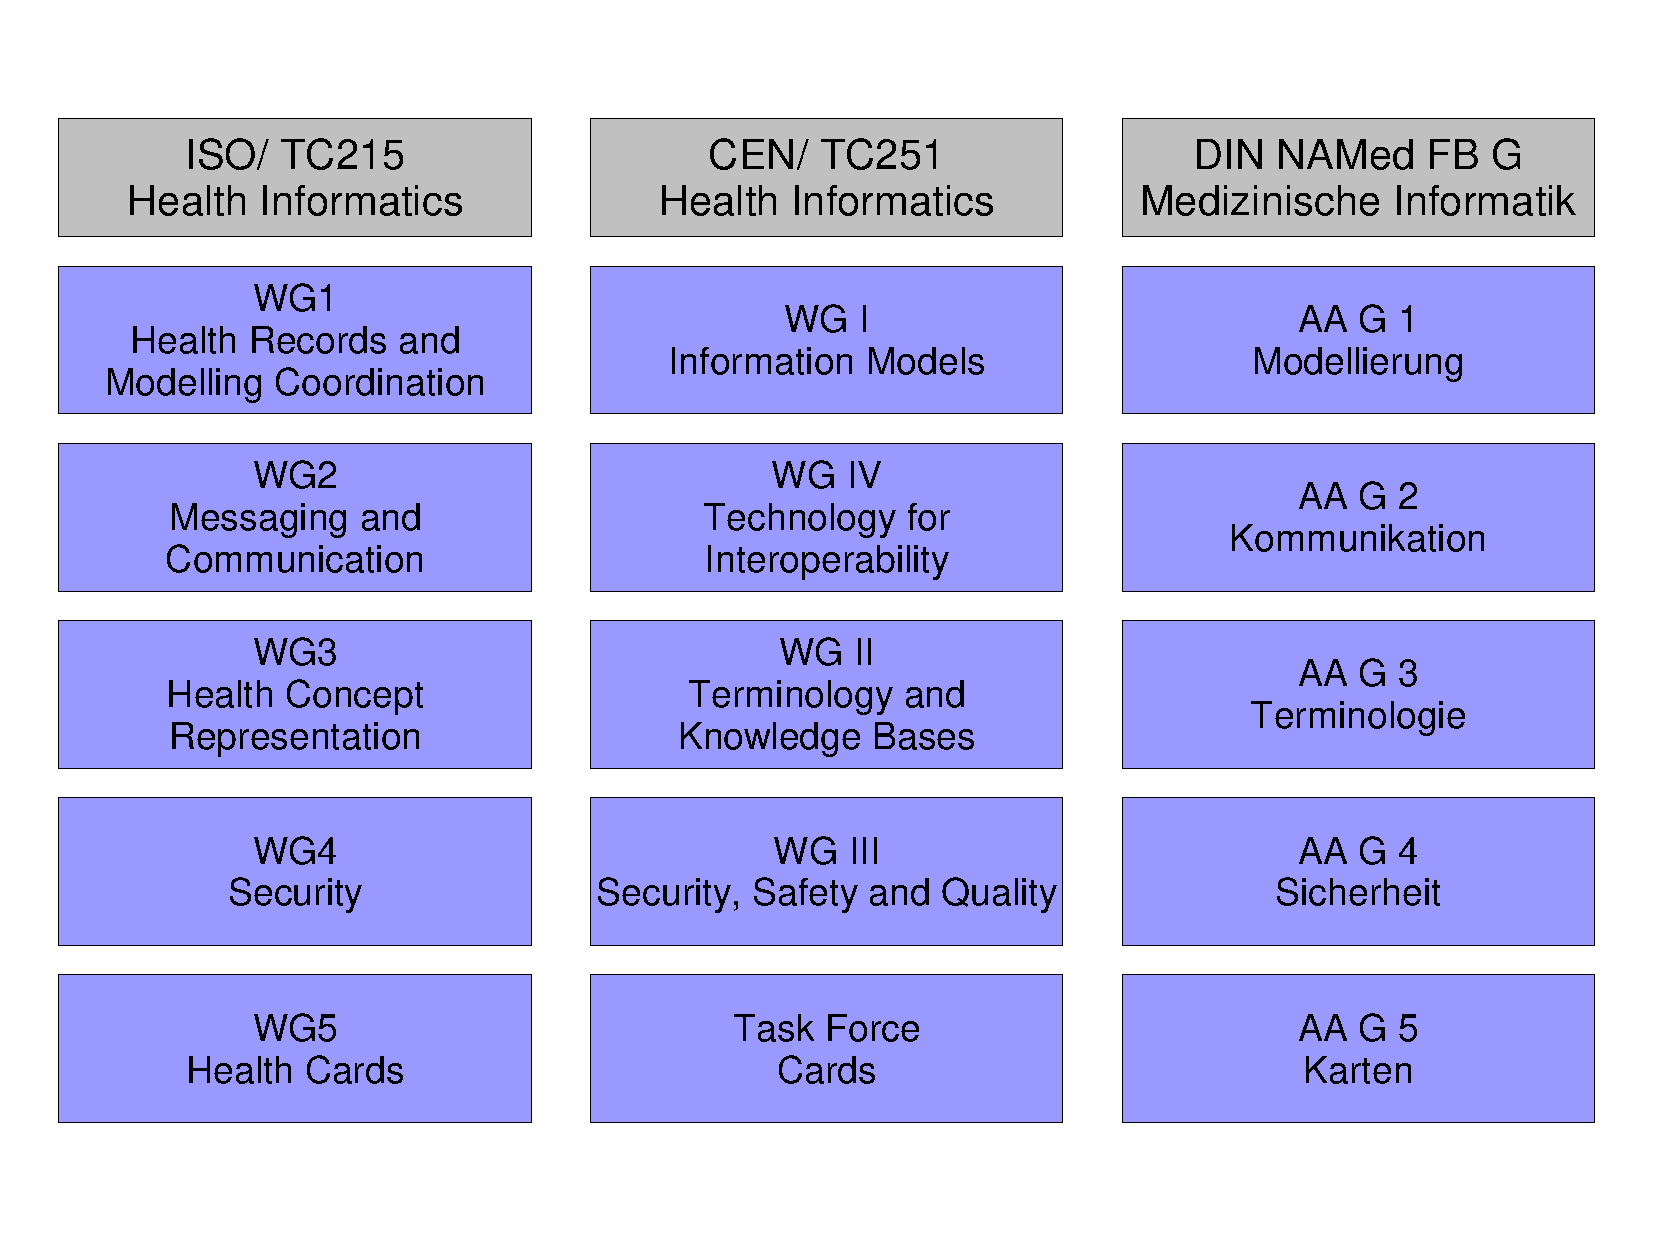
\includegraphics[scale=0.3,angle=-90]{graphic/groups.pdf}
        \caption{Medical Informatics Working Groups of DIN/ CEN/ ISO \cite{atgexpertsreport}}
        \label{groups_figure}
    \end{center}
\end{figure}

The structure of the following sections is chosen after this systematics.
Standards for \emph{Health Record Modelling} will be described first, followed
by those for \emph{Messaging and Communication} and a section on
\emph{Terminology- and Coding Systems}. \emph{Imaging-}, \emph{Health Card-}
and further standards are mentioned afterwards. General remarks on current
\emph{Standards Development Processes} follow. Reflections on the
\emph{Implications} of standards on the development of \emph{Res Medicinae}
will conclude the topic.

%
% $RCSfile: record_modelling.tex,v $
%
% Copyright (C) 2002-2008. Christian Heller.
%
% Permission is granted to copy, distribute and/or modify this document
% under the terms of the GNU Free Documentation License, Version 1.1 or
% any later version published by the Free Software Foundation; with no
% Invariant Sections, with no Front-Cover Texts and with no Back-Cover
% Texts. A copy of the license is included in the section entitled
% "GNU Free Documentation License".
%
% http://www.cybop.net
% - Cybernetics Oriented Programming -
%
% http://www.resmedicinae.org
% - Information in Medicine -
%
% Version: $Revision: 1.1 $ $Date: 2008-08-19 20:41:08 $ $Author: christian $
% Authors: Christian Heller <christian.heller@tuxtax.de>
%

\subsection{Record Modelling}
\label{record_modelling_heading}
\index{Medical Record Modelling Standards}

\input{cen_tc251}
\input{open_ehr}

%
% $RCSfile: messaging_and_communication.tex,v $
%
% Copyright (C) 2002-2008. Christian Heller.
%
% Permission is granted to copy, distribute and/or modify this document
% under the terms of the GNU Free Documentation License, Version 1.1 or
% any later version published by the Free Software Foundation; with no
% Invariant Sections, with no Front-Cover Texts and with no Back-Cover
% Texts. A copy of the license is included in the section entitled
% "GNU Free Documentation License".
%
% http://www.cybop.net
% - Cybernetics Oriented Programming -
%
% http://www.resmedicinae.org
% - Information in Medicine -
%
% Version: $Revision: 1.1 $ $Date: 2008-08-19 20:41:07 $ $Author: christian $
% Authors: Christian Heller <christian.heller@tuxtax.de>
%
\subsection{Messaging and Communication}
\label{messaging_and_communication_heading}
\index{Medical Messaging and Communication Standards}
\input{health_level_seven}
\input{healthcare_domain_task_force}
\input{edifact}
\input{x_data_carrier}
\input{healthcare_xchange_protocol}

%
% $RCSfile: terminology_systems.tex,v $
%
% Copyright (C) 2002-2008. Christian Heller.
%
% Permission is granted to copy, distribute and/or modify this document
% under the terms of the GNU Free Documentation License, Version 1.1 or
% any later version published by the Free Software Foundation; with no
% Invariant Sections, with no Front-Cover Texts and with no Back-Cover
% Texts. A copy of the license is included in the section entitled
% "GNU Free Documentation License".
%
% http://www.cybop.net
% - Cybernetics Oriented Programming -
%
% http://www.resmedicinae.org
% - Information in Medicine -
%
% Version: $Revision: 1.1 $ $Date: 2008-08-19 20:41:09 $ $Author: christian $
% Authors: Christian Heller <christian.heller@tuxtax.de>
%

\subsection{Terminology Systems}
\label{terminology_systems_heading}
\index{Medical Terminology Systems}
\index{Enumerative Scheme}
\index{Compositional Scheme}
\index{Lexical Scheme}

Besides defining the differences between a \emph{Lexicon} (list of pure words)
and \emph{Terminology} (also containing phrases), the latter sometimes called
\emph{Vocabulary}, section \ref{terminology_heading} introduced tree-like
\emph{Hierarchies} as one way to organise such sets of words or terms. Three
concrete schemes for organising terminologies were described in section
\ref{schemes_heading}: \emph{Enumerative}, \emph{Compositional} and
\emph{Lexical}. Controversial opinions about terminologies exist. Thomas Beale
wrote in \cite[December 2003]{openhealth}:

\begin{quote}
    \ldots\ trying to standardise the whole of medicine \ldots\ is a fruitless
    enterprise. Sam Heard has said this many times in presentations in
    Australia, and when he first started saying it, was amazed not to be
    stoned publicly; in fact many people have come to this conclusion through
    their own hard work, but aren't comfortable with saying it, since it goes
    against current orthodoxy (embodied in things like SNOMED CT).
\end{quote}

Nevertheless, terminologies \emph{are} a topic of research and sometimes used
in practice, as the example of ICD (see below) shows. This section therefore
briefly describes some medical terminologies and, by referring to Jeremy Rogers
\cite{rogers}, tries to assign them to one of the before-mentioned schemes.

\input{icd}
\input{opcs}
\input{read}
\input{loinc}
\input{icnp}
\input{snomed_ct}
\input{odyssee}
\input{open_galen}
\input{umls}
\input{others}

%
% $RCSfile: further_standards.tex,v $
%
% Copyright (C) 2002-2008. Christian Heller.
%
% Permission is granted to copy, distribute and/or modify this document
% under the terms of the GNU Free Documentation License, Version 1.1 or
% any later version published by the Free Software Foundation; with no
% Invariant Sections, with no Front-Cover Texts and with no Back-Cover
% Texts. A copy of the license is included in the section entitled
% "GNU Free Documentation License".
%
% http://www.cybop.net
% - Cybernetics Oriented Programming -
%
% http://www.resmedicinae.org
% - Information in Medicine -
%
% Version: $Revision: 1.1 $ $Date: 2008-08-19 20:41:06 $ $Author: christian $
% Authors: Christian Heller <christian.heller@tuxtax.de>
%

\subsection{Further Standards}
\label{further_standards_heading}

As wide as the field of medicine -- and therewith medical informatics -- is the
number of further standards that could be considered. Understandably, only a
few more examples can be mentioned here.

\input{dicom}
\input{gmdn}
\input{ncpdp}
\input{clsi}
\input{ada}
\input{cdisc}
\input{ehc}

%
% $RCSfile: standards_development.tex,v $
%
% Copyright (C) 2002-2008. Christian Heller.
%
% Permission is granted to copy, distribute and/or modify this document
% under the terms of the GNU Free Documentation License, Version 1.1 or
% any later version published by the Free Software Foundation; with no
% Invariant Sections, with no Front-Cover Texts and with no Back-Cover
% Texts. A copy of the license is included in the section entitled
% "GNU Free Documentation License".
%
% http://www.cybop.net
% - Cybernetics Oriented Programming -
%
% http://www.resmedicinae.org
% - Information in Medicine -
%
% Version: $Revision: 1.2 $ $Date: 2008-09-07 15:36:07 $ $Author: christian $
% Authors: Christian Heller <christian.heller@tuxtax.de>
%

\subsection{Standards Development}
\label{standards_development_heading}
\index{Standards Development Criticism}

Standards development in its today's form found a lot of criticism, especially
among developers of the OSS community \cite{openehrtechnical}. Their complaints
concern the:

\begin{itemize}
    \item[-] Nondisclosure and secrecy of specifications
    \item[-] Lengthy update cycles
    \item[-] Limited access to standardisation bodies
    \item[-] High membership fees
\end{itemize}

Thomas Beale who argues that the current paradigm of development of technical/
information standards were broken at the core anyway \cite{openehrtechnical},
has some more arguments, which are summarised following.

\input{unproven_specifications}
\input{static_documents}
\input{missing_methodology}
\input{arbitrary_definitions}

%
% $RCSfile: implication.tex,v $
%
% Copyright (C) 2002-2008. Christian Heller.
%
% Permission is granted to copy, distribute and/or modify this document
% under the terms of the GNU Free Documentation License, Version 1.1 or
% any later version published by the Free Software Foundation; with no
% Invariant Sections, with no Front-Cover Texts and with no Back-Cover
% Texts. A copy of the license is included in the section entitled
% "GNU Free Documentation License".
%
% http://www.cybop.net
% - Cybernetics Oriented Programming -
%
% http://www.resmedicinae.org
% - Information in Medicine -
%
% Version: $Revision: 1.1 $ $Date: 2008-08-19 20:41:07 $ $Author: christian $
% Authors: Christian Heller <christian.heller@tuxtax.de>
%

\subsection{Implication}
\label{implication_heading}
\index{Medical Informatics Standards in Res Medicinae}

The number of standards for medical informatics is huge. The fields covered by
these standards are manifold. Popular standardisation efforts dealing with the
EHR structure are \emph{Open EHR} and \emph{CEN 13606}.

The borders to messaging and communication standards are blurred. Although
\emph{HL7}'s focus lies on message exchange, it created data structures in form
of its \emph{RIM} framework, too; a newer result for document exchange is their
\emph{CDA} specification. The former two standards (\emph{CEN 13606} and
\emph{Open EHR}), on the other hand, focus on the EHR structure but offer a
communication format as well; it is called \emph{Transaction} or
\emph{Composition}, respectively. Beale concludes in \cite{openhealth}:
\textit{\ldots\ all efforts have converged independently on at least one solid
concept -- the unit of change and committal in the EHR.}

OMG's \emph{HDTF} defines interfaces for the exchange of messages, which are
grouped into special services. Some national efforts have defined their own
data exchange formats, like the \emph{xDT} standard (to become \emph{SCIPHOX})
in Germany. Yet other standards recommendations for electronic data interchange
in medicine are \emph{EDIFACT}, worked out by the UN, and \emph{HXP}, defined
by a number of medical OSS projects.

To what concerns the field of medical terminology, there exist longer-lasting
efforts like \emph{ICD}, \emph{LOINC}, \emph{SNOMED CT}, \emph{OpenGALEN} or
\emph{UMLS}. Depending on their scheme of organisation, they may be grouped
into the three categories: \emph{enumerative}, \emph{compositional} and
\emph{lexical}. A lot of time and money has been invested into them, yet only
recently, their results have been adopted by increasingly more systems. Good
acceptance and popularity was reached for the \emph{ICD} codes classification
system.

Other standards for related fields exist, among them being \emph{DICOM} for
clinical imaging and -device communication, \emph{NCPDP} for the transmission
of pharmacy data, \emph{CLSI} for clinical laboratory testing, \emph{ADA}
delivering guidelines for dental informatics or \emph{CDISC} for the exchange
of large amounts of various data between information systems.

For the purpose of this work, with a minimalistic implementation of a prototype
application, the considered (de facto) standards specifications mainly had a
helper function, giving some architectural guidance. Concerning the record
architecture, CYBOL applications follow the purely compositional principles of
CYBOP anyway, so that record modelling advices had only few implications.
CYBOI's architecture, however, is flexible enough to support many messaging
standards in the future, by simply adding the corresponding translator modules.
Existing terminologies can partly be used by associating terms appearing in
CYBOL knowledge templates with their pendants in common terminology systems.

A promising trial, in this context, would be to use CYBOL for building up new,
or structuring existing terminologies. CYBOL innately supports compositional
structures, which makes it a perfect match for compositional schemes. Further,
it allows to add meta information as well as to integrate constraints. The meta
information, which is contained in so-called \emph{property} tags of a term
(chapter \ref{cybernetics_oriented_language_heading}), at system runtime called
\emph{details}, may link to more than one superior (parent) category, thereby
placing the term simultaneously under different categories that are valid.
Thus, some problems of current terminologies (section \ref{schemes_heading})
\emph{might} get solved. But this remains to be figured out in future works
(chapter \ref{summary_and_outlook_heading}).

Standards for imaging, pharmacy- or laboratory data transfer, guidelines for
dental informatics, health card usage and related specifications will be
considered closer as soon as more application modules are developed within
\emph{Res Medicinae}.


%
% $RCSfile: realisation.tex,v $
%
% Copyright (C) 2002-2008. Christian Heller.
%
% Permission is granted to copy, distribute and/or modify this document
% under the terms of the GNU Free Documentation License, Version 1.1 or
% any later version published by the Free Software Foundation; with no
% Invariant Sections, with no Front-Cover Texts and with no Back-Cover
% Texts. A copy of the license is included in the section entitled
% "GNU Free Documentation License".
%
% http://www.cybop.net
% - Cybernetics Oriented Programming -
%
% http://www.resmedicinae.org
% - Information in Medicine -
%
% Version: $Revision: 1.1 $ $Date: 2008-08-19 20:41:08 $ $Author: christian $
% Authors: Christian Heller <christian.heller@tuxtax.de>
%

\section{Realisation}
\label{realisation_heading}
\index{Res Medicinae Steps of Realisation}

Having analysed the domain of healthcare and having investigated corresponding
standards, actual design solutions that have been tried out in the course of
this work, by implementing them in software source code, can be described in
the following sections.

%
% $RCSfile: student_works.tex,v $
%
% Copyright (C) 2002-2008. Christian Heller.
%
% Permission is granted to copy, distribute and/or modify this document
% under the terms of the GNU Free Documentation License, Version 1.1 or
% any later version published by the Free Software Foundation; with no
% Invariant Sections, with no Front-Cover Texts and with no Back-Cover
% Texts. A copy of the license is included in the section entitled
% "GNU Free Documentation License".
%
% http://www.cybop.net
% - Cybernetics Oriented Programming -
%
% http://www.resmedicinae.org
% - Information in Medicine -
%
% Version: $Revision: 1.1 $ $Date: 2008-08-19 20:41:09 $ $Author: christian $
% Authors: Christian Heller <christian.heller@tuxtax.de>
%

\subsection{Student Works}
\label{student_works_heading}
\index{Res Medicinae Student Works}

Some helpful contributions came from a number of students, collaborating within
the \emph{CYBOP} and/ or \emph{Res Medicinae} projects. The works, completed at
the \emph{Technical University of Ilmenau} (TUI), are of the three types:
\emph{Seminar Paper}, \emph{Research Project} or \emph{Diploma Thesis}, and
listed with their title and results in table \ref{works_table}.

\newpage

The first six of these works were intended to become modules for the first-trial
Java prototype of \emph{Res Medicinae}, as described in the next section.
Further works created tutorials for different base technologies, such as the
\emph{Xlibs} library of the \emph{X Window System} or \emph{Socket Communication}
mechanisms. Finally, one diploma thesis helped in defining the CYBOL language,
by creating a prototype in it.

\begin{table}[ht]
    \begin{center}
        \begin{footnotesize}
        \begin{tabular}{| p{60mm} | p{10mm} | p{35mm} |}
            \hline
            \textbf{Title} & \textbf{Type} & \textbf{Result}\\
            \hline
            A flexible Software Architecture for Presentation Layers demonstrated
            on Medical Documentation with Episodes \cite{bohl}
            & Diploma Thesis & Java application for topological documentation\\
            \hline
            A Technology-neutral Mapping Layer for Data Exchange demonstrated
            on Medical Form Printing as integrative part of an EHR \cite{kunze2003}
            & Diploma Thesis & Java application with one form and persistent storage of data\\
            \hline
            Creating a Backup Module under Consideration of Common Design Patterns
            as provided by the ResMedLib Framework \cite{behrendt}
            & Research Project & Java application for file backup\\
            \hline
            Creating Web Frontends for Scheduling and Management of administrative
            Data, based on a Webserver with JSP Technologie \cite{holzmueller2003}
            & Research Project & Apache webserver extension using Java and JSP\\
            \hline
            Creating Intuitive Frontends under Consideration of
            Internationalisation Aspects \cite{kanagasabapathi}
            & Research Project & Java application in English, German and Tamil (Latha)\\
            \hline
            Evaluating Component Technologies in the Domain of Medical Image Processing \cite{kleinschmidt}
            & Diploma Thesis & ImageJ extension for image transfer via CORBA and SOAP\\
            \hline
            X11 Architecture and XLib Functionality \cite{fache}
            & Seminar Paper & Tutorial and prototype\\
            \hline
            Communication over Sockets \cite{kiesling}
            & Seminar Paper & Tutorial and prototype\\
            \hline
            XML Parser \cite{tellhelm}
            & Seminar Paper & Code fragments\\
            \hline
            Implementation Possibilities for CYBOL Web Frontends, using
            Cybernetics Oriented Programming (CYBOP) Concepts \cite{holzmueller2005}
            & Diploma Thesis & CYBOI extensions and a more detailed CYBOL specification\\
            \hline
        \end{tabular}
        \end{footnotesize}
        \caption{Student Works \cite{cybop}}
        \label{works_table}
    \end{center}
\end{table}

%
% $RCSfile$
%
% Copyright (c) 2005-2006. Christian Heller. All rights reserved.
%
% Permission is granted to copy, distribute and/or modify this document
% under the terms of the GNU Free Documentation License, Version 1.1 or
% any later version published by the Free Software Foundation; with no
% Invariant Sections, with no Front-Cover Texts and with no Back-Cover
% Texts. A copy of the license is included in the section entitled
% "GNU Free Documentation License".
%
% http://www.cybop.net
% - Cybernetics Oriented Programming -
%
% http://www.resmedicinae.org
% - Information in Medicine -
%
% Version: $Revision$ $Date$ $Author$
% Authors: Christian Heller <christian.heller@tuxtax.de>
%

\subsubsection{First Trial}
\label{first_trial_heading}

An early trial of a \emph{Res Medicinae} module was \emph{Record}, an
application for EHR management. It was a standard Java-based system and had a
\emph{Graphical User Interface} (GUI). Its classical architecture made use of
many software patterns and was shared into the parts \emph{Domain Model},
\emph{Graphical View} and \emph{Controller}, as proposed by the equally named
pattern, abbreviated \emph{MVC}.

Later prototypes extended that architecture by applying the CYBOP concept of
\emph{Composition}. In a first step, the \emph{Hierarchical MVC} (HMVC) pattern
was used to replace the MVC pattern, resulting in nested \emph{Controllers} and
\emph{Views}. Afterwards, the principle of \emph{Hierarchy} was applied in
general, also to \emph{Domain Models} and to as many other parts as possible.

Classes as known from \emph{Object Oriented Programming} (OOP) do not represent
dynamically extensible containers but have a static structure with a fixed
number of attributes. In other words, the \emph{Hierarchy} as concept is not
inherent in OOP types. Yet abstract models as humans build them in their minds
are always based on hierarchies (section \ref{reflexions_on_concepts_heading}).
A programming language which does not consider this, does not allow users to
make full use of their modelling potential.

To eliminate this flaw and implement a hierarchical structure in the Java
prototype, a top-most super class named \emph{cybop.Model} had to be introduced.
It represented a container that had the capability to reference itself -- in
other words a \emph{Tree Structure}. As such, it offered \emph{set}, \emph{get}
and \emph{remove} methods for its elements. Since these access methods were
inherited, sub classes did not have to implement their own (for each attribute)
anymore, which saved hundreds of lines of source code.

\begin{figure}[ht]
    \begin{center}
        \includegraphics[scale=0.2]{vector/topological.eps}
        \caption{Topological Documentation}
        \label{topological_figure}
    \end{center}
\end{figure}

One of these advanced modules, to give an example, was responsible for clinical
documentation \cite{hellerbohl}, which it supported graphically, in form of
\emph{Topological Documentation} (figure \ref{topological_figure}). And, of
course, it could also manage and store patient data, in XML files.

%
% $RCSfile$
%
% Copyright (c) 2005-2006. Christian Heller. All rights reserved.
%
% Permission is granted to copy, distribute and/or modify this document
% under the terms of the GNU Free Documentation License, Version 1.1 or
% any later version published by the Free Software Foundation; with no
% Invariant Sections, with no Front-Cover Texts and with no Back-Cover
% Texts. A copy of the license is included in the section entitled
% "GNU Free Documentation License".
%
% http://www.cybop.net
% - Cybernetics Oriented Programming -
%
% http://www.resmedicinae.org
% - Information in Medicine -
%
% Version: $Revision$ $Date$ $Author$
% Authors: Christian Heller <christian.heller@tuxtax.de>
%

\subsubsection{Knowledge Separation}
\label{knowledge_separation_heading}

In the case of the first prototypes, one could still speak of true
\emph{Implementation}, because design models had to be transferred into another
form of abstract model: the Java programming language source code. Not so in
later versions of \emph{Res Medicinae}.

While the early prototypes represented the classical mix of domain knowledge
and low-level system instructions, that was eliminated later. All knowledge got
\emph{extracted} and was put into special configuration files, in \emph{CYBOL}
format (section \ref{cybol_heading}). Henceforth, these contained not only
settings like font size or colour, as known from standard applications, but the
\emph{whole} domain knowledge, including user interface- and workflow structures.

Following the explanations of section \ref{state_and_logic_heading}, the
\emph{static} knowledge was shared into different models, some representing
\emph{state-}, and others \emph{logic} knowledge. This was very much opposed to
the earlier Java implementations whose classes bundled attributes and methods.

Without the knowledge, the remaining program code looked pretty much like a
skeleton of basic system functionality. Serving as hardware interface, it
concentrated memory- and signal handling in one place -- exactly those things
which section \ref{statics_and_dynamics_heading} called \emph{Dynamics}.
Additionally, that remaining system had the ability to interpret knowledge,
which is why it was called \emph{CYBOI} (interpreter). One could, in some way,
compare it with what the \emph{Java Virtual Machine} (JVM) is for Java, only
that CYBOI processed knowledge given in form of CYBOL templates, which look
different than Java source code.

CYBOI needed an \emph{XML Parser} in order to be able to read the knowledge
contained in CYBOL files. The decision here fell on Apache's \emph{Xerces}
\cite{xerces}, because one of its versions is implemented in Java.

%
% $RCSfile: reimplementation.tex,v $
%
% Copyright (C) 2002-2008. Christian Heller.
%
% Permission is granted to copy, distribute and/or modify this document
% under the terms of the GNU Free Documentation License, Version 1.1 or
% any later version published by the Free Software Foundation; with no
% Invariant Sections, with no Front-Cover Texts and with no Back-Cover
% Texts. A copy of the license is included in the section entitled
% "GNU Free Documentation License".
%
% http://www.cybop.net
% - Cybernetics Oriented Programming -
%
% http://www.resmedicinae.org
% - Information in Medicine -
%
% Version: $Revision: 1.1 $ $Date: 2008-08-19 20:41:08 $ $Author: christian $
% Authors: Christian Heller <christian.heller@tuxtax.de>
%

\subsection{Reimplementation}
\label{reimplementation_heading}
\index{CYBOP}
\index{Itemisation}
\index{Composition}
\index{Bundling of Attributes and Methods}
\index{Container Inheritance}
\index{CYBOL}
\index{CYBOI}
\index{OOP}
\index{Java Programming Language}
\index{C++ Programming Language}
\index{C Programming Language}
\index{Operating System}
\index{OS}
\index{XML}
\index{Graphical User Interface}
\index{GUI}
\index{empty}
\index{Abstract Windowing Toolkit}
\index{AWT}
\index{Swing}
\index{Qt}
\index{wxWindows}
\index{Gimp Toolkit}
\index{GTK}
\index{GNU/Linux}
\index{XFree86}
\index{X-Library}
\index{Xlib}
\index{Textual User Interfaces}
\index{TUI}
\index{Web User Interfaces}
\index{WUI}
\index{Socket Communication Mechanisms}

The architecture-advanced prototype of the \emph{Record} module had \emph{much}
less functionality than earlier ones, in fact not much more than starting a
graphical frame with menu bar and exiting the application again. This was so,
because yet before all domain knowledge could be extracted into CYBOL, another
issue turned up:

CYBOP modelling concepts like \emph{Itemisation} or \emph{Composition} are an
integral part of the CYBOL knowledge representation language. Other concepts
like the \emph{Bundling} of attributes and methods, property- and container
\emph{Inheritance}, as known from \emph{Object Oriented Programming} (OOP),
were considered unfavourable (section \ref{object_oriented_programming_heading})
and neither to be used in CYBOL, nor in the CYBOI interpreter. Consequently,
OOP languages like Java or C++ were not suitable for CYBOI any longer. A slim
and fast language, close to hardware and fast in processing CYBOL was needed.

Having such requirements, one of the first candidates coming to mind was the
\emph{C} programming language. It is \emph{high-level} enough to permit fast
programming and \emph{low-level} enough to connect efficiently to hardware or
an \emph{Operating System} (OS). Many OS are written in C themselves, anyway.
CYBOI was therefore reimplemented in C, which hasn't changed since. What has
changed and is changing all the time is its functionality, an overview of which
was given in chapter \ref{cybernetics_oriented_interpreter_heading}.

CYBOL sticks to the XML specification and standard XML parsers can be used to
process and validate it. However, for reasons of performance and better
integration, and due to the very limited vocabulary (set of possible tags and
attributes), special parsing procedures were written and adapted to CYBOI.

Another problem that had to be solved was \emph{Graphical User Interface} (GUI)
handling. While the Java-implemented CYBOI could make use of the
\emph{Abstract Windowing Toolkit} (AWT)/ Swing, the C-implemented CYBOI did not
have such functionality at first. Toolkit candidates like \emph{Qt} \cite{qt}
or \emph{wxWindows} \cite{wxwidgets}, being implemented in C++, were out. Other
GUI frameworks like the \emph{Gimp Toolkit} (GTK) \cite{gtk}, written in C,
were considered cumbersome to cope with so that finally, the decision was taken
to use low-level graphics drawing routines. For CYBOI, being developed on a
\emph{GNU/Linux} OS \cite{linux}, that meant using \emph{XFree86's}
\cite{xfree86} \emph{X-Library} (Xlib) functionality directly. The necessary
effort for transforming hierarchical CYBOL models into GTK- or other toolkit
structures was estimated to be equal or even higher than translating them into
Xlib functionality right away. At the time of writing this work, implementation
is in progress but not completed.

Similar implementations are necessary for \emph{Textual User Interfaces} (TUI),
\emph{Web User Interfaces} (WUI) and \emph{Socket Communication Mechanisms},
the latter two being already finished in a first version. Further development
activities may for instance enable CYBOI to run on other platforms and integrate
more hardware-driving functionality, to get independent from underlying OS.

While the CYBOL specification can be considered quite mature, CYBOI, as could
be seen, will need plenty of extensions and additions in future, in order to
leave its prototype stage and become fully usable.

%
% $RCSfile$
%
% Copyright (c) 2005-2006. Christian Heller. All rights reserved.
%
% Permission is granted to copy, distribute and/or modify this document
% under the terms of the GNU Free Documentation License, Version 1.1 or
% any later version published by the Free Software Foundation; with no
% Invariant Sections, with no Front-Cover Texts and with no Back-Cover
% Texts. A copy of the license is included in the section entitled
% "GNU Free Documentation License".
%
% http://www.cybop.net
% - Cybernetics Oriented Programming -
%
% http://www.resmedicinae.org
% - Information in Medicine -
%
% Version: $Revision$ $Date$ $Author$
% Authors: Christian Heller <christian.heller@tuxtax.de>
%

\subsubsection{Module Modelling}
\label{module_modelling_heading}

When CYBOI had become more stable (besides the extensions that were -- and are
-- frequently implemented, development could focus on the actual application
again. From now on, \emph{Res Medicinae} modules only had to be \emph{modelled}
in CYBOL, but no longer had to be \emph{coded} in a programming language. The
designed state- and logic knowledge, existing in form of CYBOL templates,
already represented the complete application; no further implementation phase
was needed.

\begin{figure}[ht]
    \begin{center}
        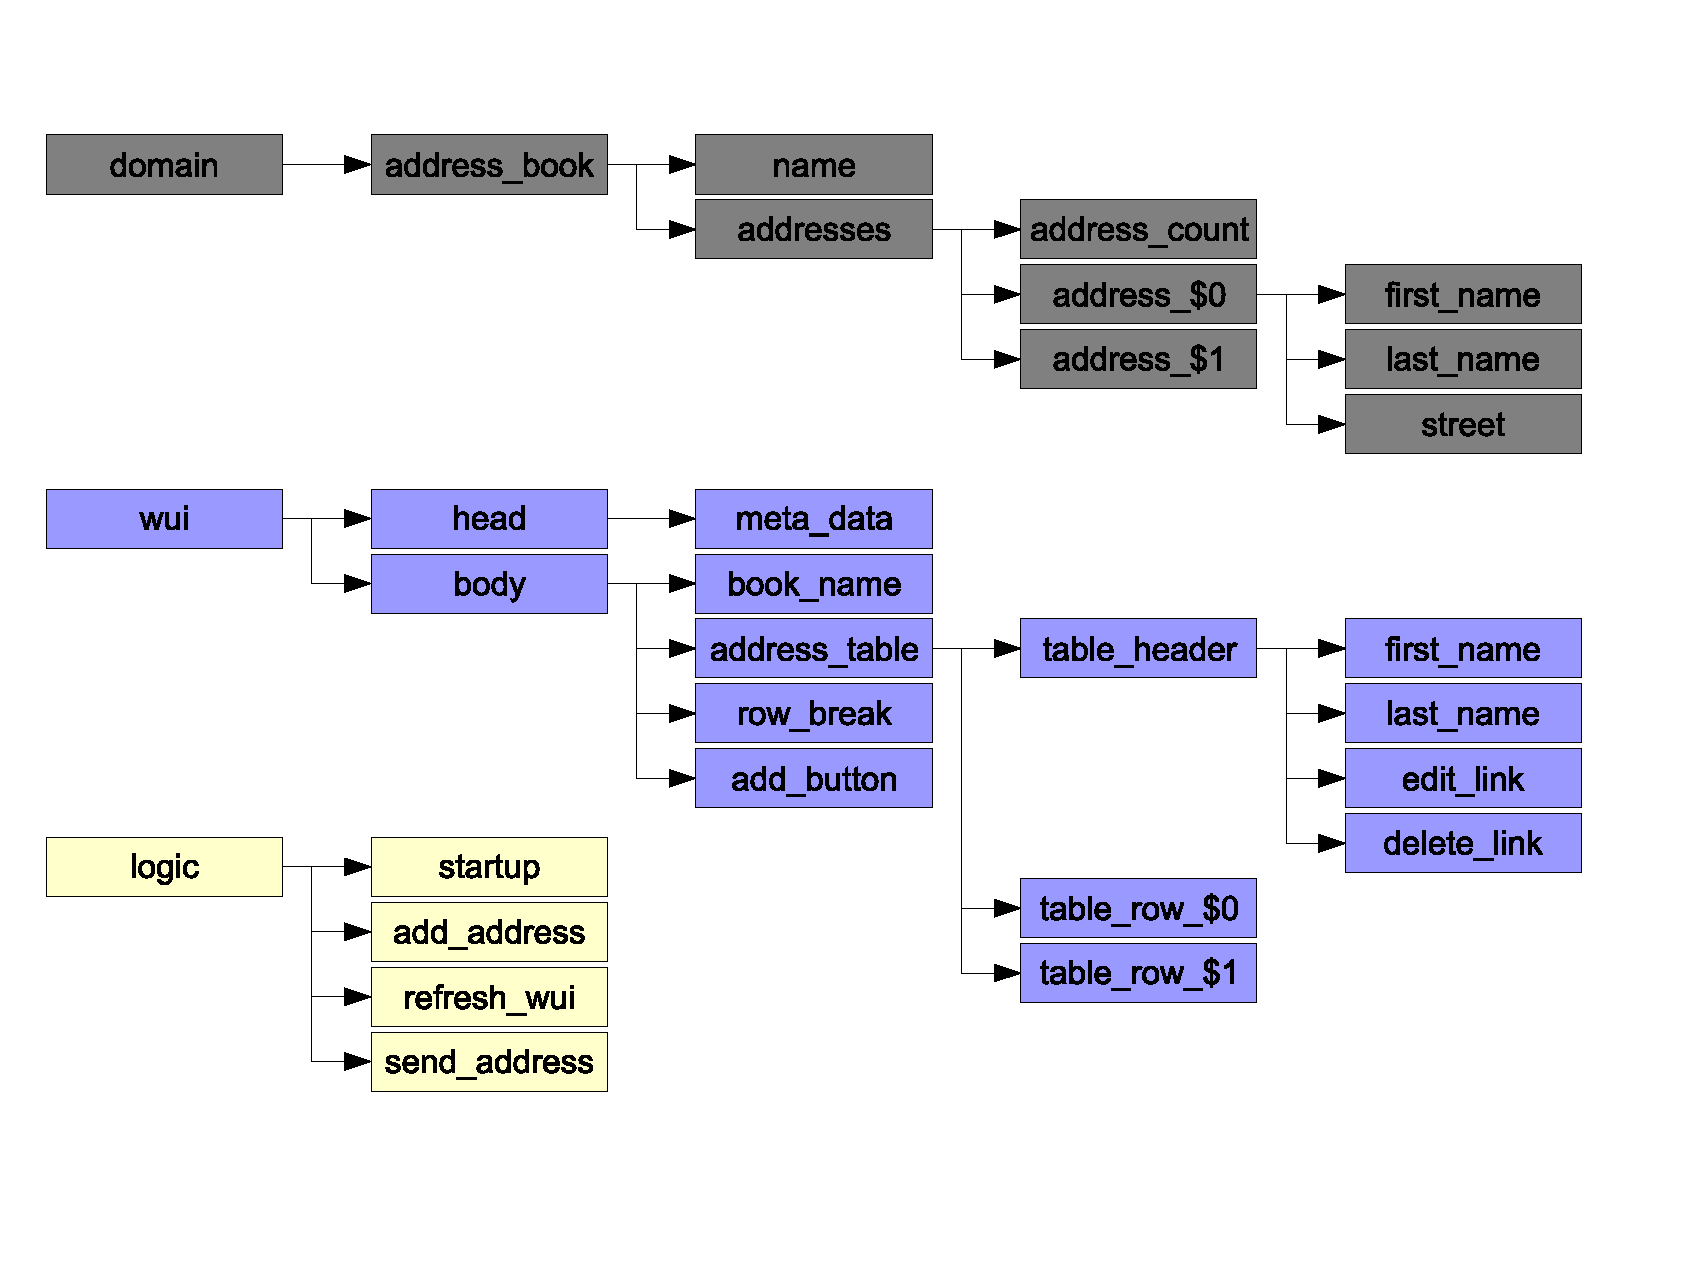
\includegraphics[scale=0.2]{vector/radesign.eps}
        \caption{ResAdmin Knowledge Models}
        \label{radesign_figure}
    \end{center}
\end{figure}

Due to the tremendous complexity of an \emph{Electronic Health Record} (EHR),
only a very small part of its data could be considered for the application
prototype. Administrative data like a person's name or address are standard
information found in all EHRs. A corresponding module named \emph{ResAdmin}
\cite{holzmueller2005} was therefore elected to be realised first. Its models
belong to three categories: \emph{Domain}, \emph{Web User Interface} (WUI) and
\emph{Logic} (figure \ref{radesign_figure}).

The addresses contained in the \emph{domain} branch of the knowledge tree are
manipulated across \emph{Hyper Text Markup Language} (HTML) \emph{User Interface}
(UI) models belonging to the \emph{web} branch of that same tree. An example
structure of a knowledge tree was shown in figure \ref{mvctree_figure}. Every
action model that a user can trigger through the WUI exists as part of the
\emph{logic} branch of the knowledge tree.

Independently of what kind of knowledge model (state or logic) was created,
ontological principles were strictly followed. Most importantly, relations
within a hierarchical model were always \emph{unidirectional}, that is from a
\emph{Whole-} to its \emph{Part} models, but never the other way around.
Additionally, however, logic models may reference and access runtime state
models.

Some of the logic models represent \emph{Translators} (compare section
\ref{communication_model_heading}). They extract address information
residing in the domain- and copy them to the web model, which is afterwards
sent to the human user as communication partner. This principle holds true for
the communication between application systems, only that then other than web
models are used as communication format. The vision to make all communication
channels really \emph{transparent} and easy to handle for the user now seems to
be coming true.



